\documentclass[11pt]{amsart}

\usepackage[margin=1.15in]{geometry}
\usepackage{amsmath,amssymb,mathtools}
\usepackage{booktabs}
\usepackage{array}
\usepackage{graphicx}
\usepackage{xcolor}
\usepackage{enumitem}
\definecolor{linkblue}{RGB}{25,60,120}
\definecolor{draftred}{RGB}{140,25,25}
\usepackage[colorlinks=true,linkcolor=linkblue,citecolor=linkblue,urlcolor=linkblue]{hyperref}
\hypersetup{
  pdftitle={New constructions, obstructions, and multiplier structure for Erdos Problem 634},
  pdfauthor={Jan Philipp Harries},
  pdfsubject={Triangle tilings by congruent triangles},
  pdfkeywords={triangle tilings, congruent triangles, Erdos problem 634, exact computation, numerical semigroups}
}

\newtheorem{theorem}{Theorem}
\newtheorem{lemma}[theorem]{Lemma}
\newtheorem{proposition}[theorem]{Proposition}
\newtheorem{corollary}[theorem]{Corollary}
\theoremstyle{definition}
\newtheorem{definition}[theorem]{Definition}
\theoremstyle{remark}
\newtheorem{remark}[theorem]{Remark}

\newcommand{\Z}{\mathbb Z}
\newcommand{\Q}{\mathbb Q}
\newcommand{\N}{\mathbb N}
\newcommand{\Nzero}{\mathbb N_0}
\newcommand{\Sset}{\mathcal S}
\newcommand{\Aset}{\mathcal A}
\newcommand{\pathcode}[1]{\nolinkurl{#1}}

\title[Progress toward Erd\H{o}s Problem 634]{New constructions, obstructions, and multiplier
structure for Erd\H{o}s Problem 634}

\author{Jan Philipp Harries}
\thanks{ellamind GmbH, Bremen, Germany.
\textit{E-mail address:} \href{mailto:jan@ellamind.com}{jan@ellamind.com}}

\date{July 27, 2026}

\subjclass[2020]{Primary 52C20; Secondary 51M04, 11D07, 11D09, 68V05}
\keywords{triangle tilings, congruent triangles, Erd\H{o}s problem 634,
computer-assisted proof, numerical semigroups}

\raggedbottom

\begin{document}

\begin{abstract}
Let $\Sset$ be the set of integers $N>1$ for which some nondegenerate
Euclidean triangle can be tiled by $N$ congruent triangles.  This paper
continues the determination of the prime members of $\Sset$ and develops a
framework for the full Erd\H{o}s Problem~634.  We give exact-coordinate
certificates proving $88,189\in\Sset$, and an
exact computer-assisted exhaustion proving $33\notin\Sset$ whose complete
branch tree is exported as a finite refutation certificate and validated by
an independently written checker.  The $189$-tiling settles the first unknown
multiplier on the Group~1 ray $21n^2$ and, with known constructions, shows that
every multiplier $n\ge2$ occurs on that ray.

For a primitive $120^\circ$ tile with sides
$c^2=a^2+ab+b^2$, we introduce a Laurent-polynomial boundary invariant whose
quotient is $\Z/(3ab)$.  It subsumes the ideal-membership obstructions from
the known signed boundary characters and gives the exact arithmetic necessity
on all six Group~2 target shapes.  We
also prove that every Group~2 multiplier set is a numerical semigroup with an
explicit finite generator window.  A trapezoid construction improves
known sufficient thresholds; exact positive certificates and a
one-implementation exhaustive search determine the entire one-leg family for
the tile $(3,5,7)$.  Supporting transfer and ordered-segment results isolate,
but do not solve, the remaining geometric seam-propagation problem.  Detailed
computational qualifications, a result ledger, and a provisional programme
below $200$ are separated into the appendices.
\end{abstract}

\maketitle

\section{Introduction}\label{sec:intro}

An integer $N>1$ belongs to $\Sset$ if at least one nondegenerate triangle
admits a dissection into $N$ pairwise interior-disjoint triangles congruent to
one another; reflections are allowed and the dissection need not be
edge-to-edge.  Erd\H{o}s Problem~634 asks for a characterization of $\Sset$
\cite{EP634,Soifer09}.  Classical constructions give
\[
 n^2,\qquad 2n^2,\qquad 3n^2,\qquad 6n^2,\qquad n^2+m^2\in\Sset
\]
in their natural ranges \cite{SWW91,Soifer09}.  Recent classification theorems
of Laczkovich, Beeson, and Zhang reduce all remaining possibilities to a small
number of geometric branches \cite{Lacz95,Lacz12,BLZ633,BZRat}.

This paper is a sequel to \cite{HarriesPrime}.  Three contemporaneous
manuscripts independently obtained the prime classification
\[
             p=2,\qquad p=3,\qquad\text{or}\qquad p\equiv1\pmod4.
\]
They use complementary direct and classification-based arguments
\cite{GeorgePrime,HarriesPrime,BeesonAllPrime,BeesonPrime}; no claim of
exclusive priority is intended.  Beeson's four scalene $120^\circ$ count
formulae also confirm four rows of Table~\ref{tab:group2}.  These manuscripts
settle only the prime subproblem; the full characterization of $\Sset$ remains
open.

The full problem is substantially harder than the prime case.  Arithmetic
classification places a candidate on a square ray $N=Cm^2$, but it usually
does not decide which multipliers $m$ are geometrically realizable.  The three
principal contributions of this paper are:
\begin{enumerate}[leftmargin=2.2em]
\item exact, independently checkable certificates for the new counts $88$
      and $189$, together with an exclusion of $33$ whose complete search
      tree is exported as a finite refutation certificate and validated by
      an independently written checker;
\item a single Laurent quotient that closes the
      $\chi(j,m)=(-1)^jz^m$ ideal-membership programme for $120^\circ$ tiles;
      and
\item additive and finite-generation structure for the multiplier sets,
      turning every Group~2 ray into finitely many exact tiling questions.
\end{enumerate}
Exact trapezoid, transfer, and ordered-segment results support this programme
and identify the remaining geometric obstruction.

\paragraph{Evidence levels.}
A result labelled \emph{proved} has a mathematical proof here or in a cited
source.  An \emph{independently certified computer-assisted theorem} depends
on an exact exhaustive search whose complete branch tree has been exported as
a finite refutation certificate and accepted by a checker written from the
certificate specification alone, sharing no code with the search
(Appendix~\ref{app:certificates}).  For such a result the search program is
not part of the proof surface: the certificate, the checker, and the lemmas
of Appendix~\ref{app:negative} are.  A plain \emph{computer-assisted theorem}
depends on an exact exhaustive search for which no such certificate has been
exported, so it rests on one implementation, and its completeness argument
and reproducibility data in Appendix~\ref{app:verification} are the proof
surface.  A \emph{verified certificate} is a positive tiling rechecked from
exact coordinates, independently of the search history.  The label
\emph{conditional} is reserved for consequences of the unfinished
forced-layer lemma in Appendix~\ref{app:conditional}.  No conditional
statement is used to prove an unconditional result.

\section{The classified branches and the prime case}\label{sec:framework}

We use the classification in the same form as \cite{HarriesPrime}, but we
now state the imported statements on which every arithmetic branch of this
paper rests.  Throughout, $T$ is the tiled triangle and $R$ the tile, with
angles $\alpha,\beta,\gamma$ opposite the sides $a,b,c$; \emph{commensurable
angles} means that all three tile angles are rational multiples of $\pi$;
reflections are allowed and no tiling is assumed edge-to-edge.  All
statements below are quoted or transcribed from the cited versions; the
version pins and the logical role of each are collected in the dependency
ledger, Tables~\ref{tab:ledger} and~\ref{tab:ledgerb}.

\subsection{Imported classification statements}\label{sec:imports}

The classification splits by the shape of the target, not by the tile.  We
use it in four pieces.

\begin{theorem}[Imported; reptilings, {\cite{SWW91}}, as restated in
{\cite[Thm.~4]{BLZ633}} and tabulated in {\cite[Table~3]{Beeson7}}]
\label{thm:imp-reptile}
If $T$ is similar to $R$, then $N\in\{n^2\}\cup\{e^2+f^2\}\cup\{3n^2\}$, the
second family occurring exactly for right tiles and the third for the
$(\pi/6,\pi/3,\pi/2)$ tile; every value in these families occurs.
\end{theorem}

\begin{theorem}[Imported; commensurable tiles, {\cite[Thm.~3 and Table~3]{Beeson7}}]
\label{thm:imp-comm}
If all three angles of $R$ are rational multiples of $\pi$, then the pair
$(T,R)$ and $N$ correspond to one of the eight lines of
\cite[Table~3]{Beeson7}; in particular
\[
   N\in\{n^2\}\cup\{e^2+f^2\}\cup\{2n^2\}\cup\{3n^2\}\cup\{6n^2\}.
\]
\end{theorem}

\begin{theorem}[Imported; non-isosceles targets, Laczkovich,
{\cite[Thm.~4.1]{Lacz95}}, as tabulated in {\cite[Table~4]{Beeson7}} and
restated in {\cite[Thm.~9]{BLZ633}}]
\label{thm:imp-nonisosceles}
Suppose $T$ is not isosceles, $T$ is not similar to $R$, and the angles of
$R$ are not all rational multiples of $\pi$.  Then, after possibly
interchanging $(\alpha,a)$ with $(\beta,b)$, exactly one of the following
holds:
\begin{enumerate}[label=\textup{(\alph*)}]
\item $3\alpha+2\beta=\pi$ and $T$ has angles $(2\alpha,\beta,\alpha+\beta)$
      or $(2\alpha,\alpha,2\beta)$ \textup{(Group 1, shapes 1--2)};
\item $\gamma=2\pi/3$ and $T$ has angles $(\alpha,2\alpha,3\beta)$,
      $(\alpha,2\beta,2\alpha+\beta)$, $(\alpha,\alpha+\beta,\alpha+2\beta)$
      or $(2\alpha,2\beta,\alpha+\beta)$ \textup{(Group 2, rows II--V)}.
\end{enumerate}
\end{theorem}

\begin{theorem}[Imported; isosceles non-equilateral targets,
{\cite[Thm.~3]{BeesonPrime}}]\label{thm:imp-isosceles}
Let $T$ be isosceles and not equilateral, $N$-tiled by $R$, and suppose $T$
is not similar to $R$.  Then, possibly after renaming $\alpha$ and $\beta$:
\textup{(i)} $\gamma=2\alpha$, or $\gamma=\pi/2$, or $\gamma=2\pi/3$, or
$3\alpha+2\beta=\pi$; \textup{(ii)} unless $\gamma=\pi/2$, the angles of $R$
are incommensurable; \textup{(iii)} the base angles of $T$ are $\alpha$,
$\beta$, or $\alpha+\beta$.
\end{theorem}

\begin{theorem}[Imported; equilateral targets, Laczkovich,
{\cite[Thm.~3.3]{Lacz12}}]\label{thm:imp-equilateral}
Let $T$ be equilateral and $N$-tiled by $R$.  If $\alpha$ is not a rational
multiple of $\pi$, then $\gamma=\pi/3$ or $\gamma=2\pi/3$.  If $\alpha$ is a
rational multiple of $\pi$, then $R$ is equilateral, or the right triangle
with a $\pi/6$ angle, or the isosceles triangle with a $\pi/6$ apex.
\end{theorem}

\noindent The statement above is the form in which \cite[Thm.~3.3]{Lacz12}
is invoked in the proof of \cite[Thm.~11]{BeesonPrime}, which is the source
we read; the 2012 paper's own wording was not re-verified here.  Note also
that \cite[Lemma~7.1]{Lacz12} is the step patched in the appendix of
\cite{BZRat}.

\begin{theorem}[Imported; right tiles, {\cite[Thm.~7.10]{BeesonIso}}]
\label{thm:imp-right}
Let $N>1$ and let $R$ be right-angled with angles $(\alpha,\beta,\pi/2)$.
Then an isosceles $T$ is $N$-tileable by $R$ only in the following cases:
$N/2$ is a square (any isosceles $T$); $N/2=r^2+p^2$ (base angles $\beta$
with $\tan\beta=r/p$, and this is an equivalence); $N$ is a square (right
isosceles $T$); $N=6k^2$ (base angles $\pi/6$).  If none of these applies,
no isosceles $T$ can be $N$-tiled by any right tile.
\end{theorem}

\subsection{Imported rationality and parametrization statements}
\label{sec:imports-rat}

Each branch needs its own licence to normalize the tile to an integer
triple.  There are three such licences and they are logically independent.

\begin{theorem}[Imported; Beeson--Zhang rationality,
{\cite[Thm.~1.2]{BZRat}}, quoted as {\cite[Thm.~1]{Zhang25}}]
\label{thm:imp-rat}
Let $T$ be tiled by $R$ with $R$ not similar to $T$, $R$ not a right
triangle, and $R$ having incommensurable angles.  Then $R$ has commensurable
sides.
\end{theorem}

Theorem~\ref{thm:imp-rat} is what licenses the integer normalization of the
Group~2 tile recorded in \eqref{eq:eisenstein} below.  For Group~1 we do not
need it: rationality there is internal to \cite{Beeson2229}.

\begin{theorem}[Imported; rational Group-1 tile,
{\cite[Thm.~3]{Beeson2229}}]\label{thm:imp-g1rat}
Let $T$ be $N$-tiled by a tile with sides $(a,b,c)$ and angles
$(\alpha,\beta,\gamma)$, let $3\alpha+2\beta=\pi$, and suppose $T$ is not
similar to the tile.  Then the tile is rational; specifically $s=a/c$ and
$b/c$ are rational.
\end{theorem}

With $s=a/c=p/q$ in lowest terms, $0<p<q$, and $b/c=1-s^2$
\cite[Lemma~2]{Beeson2229}, the tile is a positive rational multiple of
$(pq,\,q^2-p^2,\,q^2)$, and that triple is primitive: a prime dividing $q^2$
and $pq$ divides $q$, hence divides $q^2-p^2$ and therefore $p$, contrary to
$\gcd(p,q)=1$.  This is the normalization used in
Section~\ref{sec:otherbranches}.

\begin{theorem}[Imported; the $\gamma=2\alpha$ branch,
{\cite[Thm.~10.5, Lemma~11.2, Lemma~11.4]{BeesonIso}}]
\label{thm:imp-g2a}
Let $T$ be isosceles with base angles $\alpha$, $\alpha/\pi\notin\Q$, and
let $T$ be $N$-tiled by a tile with angles $(\alpha,\beta,2\alpha)$.  Then
the tile is rational; after scaling, its sides are integers without a common
factor and
\[
   (a,b,c)=(u^2,\ v^2-u^2,\ uv)
\]
for coprime integers $u,v$ with $u<v<2u$; and the equal side $X$ of $T$
satisfies the area equation $X^2=Nab$.
\end{theorem}

\noindent The area equation is elementary---both areas carry the factor
$\sin(\alpha+\beta)$---so only the rationality and the parametrization are
genuine imports.

\subsection{The two groups}\label{sec:twogroups}

Putting the pieces together, the branches that survive for a target that is
neither a reptile nor covered by the commensurable or right-tile lists are
the two groups
\[
  3\alpha+2\beta=\pi \quad\text{(Group 1)},\qquad
  \gamma=\frac{2\pi}{3}\quad\text{(Group 2)},
\]
together with the two isolated branches $\gamma=2\alpha$ (isosceles target)
and $\gamma=\pi/3$ (equilateral target).  Proposition~\ref{prop:reduction33}
below carries out the resulting case division in full for $N=33$.  The Group~2 tile can consequently be scaled to a primitive
integer triple
\begin{equation}\label{eq:eisenstein}
       c^2=a^2+ab+b^2,\qquad \gcd(a,b,c)=1,
\end{equation}
where $c$ is opposite the $120^\circ$ angle.

\begin{lemma}[Arithmetic of primitive Group~2 triples]\label{lem:g2-units}
For a primitive positive solution of \eqref{eq:eisenstein}, the integers
$a,b,c$ are pairwise coprime, $3\nmid c$, and both $c$ and $a-b$ are units
modulo $3ab$.
\end{lemma}

\begin{proof}
If a prime divides any two of $a,b,c$, the norm equation makes it divide the
third, contrary to primitivity.  Thus the triple is pairwise coprime.  If
$3\mid c$, reduction modulo $3$ gives $a\equiv b\pmod3$.  If $3\mid a$,
then also $3\mid b$, again impossible.  Otherwise write $b=a+3t$; then
\[
 a^2+ab+b^2=3(a^2+3at+3t^2)\equiv3\pmod9,
\]
whereas $c^2\equiv0\pmod9$, a contradiction.  Hence $3\nmid c$.  Finally,
pairwise coprimality gives $\gcd(a-b,ab)=1$, and
$(a-b)^2\equiv c^2\not\equiv0\pmod3$ gives $3\nmid(a-b)$.  The stated unit
claims follow.
\end{proof}

\begin{lemma}[Arithmetic of primitive $60^\circ$ triples]\label{lem:g60-units}
Let $a,b,c$ be positive integers with
\[
       c^2=a^2-ab+b^2,\qquad\gcd(a,b,c)=1 .
\]
Then $a,b,c$ are pairwise coprime, $3\nmid c$, $3\nmid(a+b)$, and both
$c$ and $a+b$ are units modulo $3ab$.
\end{lemma}

\begin{proof}
If a prime $\ell$ divides two of $a,b,c$, then the norm equation in the
forms
\[
 c^2=a^2-ab+b^2,\qquad b^2=c^2-a^2+ab,\qquad a^2=c^2+ab-b^2
\]
makes $\ell$ divide the square of the third, hence the third, contrary to
primitivity.  Thus the triple is pairwise coprime.

Next, $a^2-ab+b^2=(a+b)^2-3ab$, so
\[
             c^2\equiv(a+b)^2\pmod3,
\]
and therefore $3\mid c$ if and only if $3\mid(a+b)$.  (Equivalently: among the
nine residue pairs $(a,b)$ modulo $3$, exactly the three with
$a+b\equiv0\pmod3$ make $a^2-ab+b^2$ divisible by $3$.)  Suppose
$3\mid(a+b)$, hence $3\mid c$.  Then $3\nmid a$, since $3\mid a$ together with
$3\mid(a+b)$ would give $3\mid b$, contradicting $\gcd(a,b)=1$.  Write
$b=-a+3k$ with $k\in\Z$; then
\[
 c^2=a^2-a(-a+3k)+(-a+3k)^2=3a^2-9ak+9k^2 .
\]
As $3\nmid a$ we have $a^2\equiv1\pmod3$, so $c^2\equiv3a^2\equiv3\pmod9$,
whereas $3\mid c$ forces $9\mid c^2$.  This contradiction gives
$3\nmid(a+b)$ and $3\nmid c$.

Finally, pairwise coprimality gives $\gcd(c,ab)=1$, and with $3\nmid c$ the
residue of $c$ is a unit modulo $3ab$.  Likewise
$\gcd(a+b,a)=\gcd(b,a)=1$ and $\gcd(a+b,b)=\gcd(a,b)=1$, so
$\gcd(a+b,ab)=1$; with $3\nmid(a+b)$ the residue of $a+b$ is a unit modulo
$3ab$ as well.
\end{proof}

The six Group~2 target shapes are listed in Table~\ref{tab:group2}.  We use
\[
             U=a+2b,\qquad V=2a+b,\qquad W=a+b.
\]
Rows I--V are the five non-equilateral shapes in Laczkovich's table, with
the interchange $(\alpha,a)\leftrightarrow(\beta,b)$ allowed; row E is the
equilateral target.

\begin{table}[ht]
\centering
\small
\renewcommand{\arraystretch}{1.12}
\begin{tabular}{@{}c>{\raggedright\arraybackslash}p{0.29\linewidth}
>{\raggedright\arraybackslash}p{0.23\linewidth}
>{\raggedright\arraybackslash}p{0.25\linewidth}@{}}
\toprule
row & target data & necessary scale condition & tile count \\
\midrule
I   & sides $k(c,c,U)$                & $b\mid k$ & $m^2bU$ \\
II  & sides $k(c^2,Uc,3bW)$           & none beyond $k\in\N$ & $3m^2UW$ \\
III & sides $k(ac,bV,Wc)$              & none beyond $k\in\N$ & $m^2VW$ \\
IV  & sides $k(a,c,W)$                 & $b\mid k$ & $m^2bW$ \\
V   & sides $k(aU,bV,c^2)$             & none beyond $k\in\N$ & $m^2UV$ \\
E   & equilateral, side $L$            & $ab\mid L$ & $m^2ab$ \\
\bottomrule
\end{tabular}
\caption{The Group~2 rays.  In rows I and IV, $k=bm$; in row E,
$L=abm$.  In the other rows $m=k$.  The arithmetic necessity is proved in
Section~\ref{sec:laurent}; known constructions realize a tail, but generally
not every multiplier.}\label{tab:group2}
\end{table}

The prime case is now unusually well cross-checked.  The proof in
\cite{HarriesPrime} uses scale integrality and the count formulae;
\cite{GeorgePrime} adds a signed boundary obstruction; and
\cite{BeesonAllPrime} derives the four scalene Group~2 cases independently,
delegating the other branches to the cited classification papers.  We do not
repeat that proof.  Its role here is to close one slice of $\Sset$ and to fix
the imported framework on which the composite investigation rests.

None of the prime-case results is used in any proof in this paper.
Theorem~\ref{thm:no33}, Proposition~\ref{prop:reduction33} and the ledger of
Appendix~\ref{app:ledger} import only the classification, rationality and
construction statements of Sections~\ref{sec:imports}--\ref{sec:imports-rat}
and of Tables~\ref{tab:ledger} and~\ref{tab:ledgerb}; the prime classification enters solely as
context and as the corroborating rows of that ledger.

\section{New exact tilings and the exclusion of 33}\label{sec:newcounts}

\begin{theorem}[Verified exact certificates]\label{thm:88189}
The following tilings exist.
\begin{enumerate}[label=\textup{(\roman*)}]
\item A triangle with side lengths $(21,55,56)$ is tiled by $88$ congruent
      copies of the triangle $(3,5,7)$.
\item A triangle with side lengths $(36,36,63)$ is tiled by $189$ congruent
      copies of the triangle $(2,3,4)$.
\end{enumerate}
Consequently $88m^2,189m^2\in\Sset$ for every $m\ge1$.
\end{theorem}

\begin{proof}
The exact vertex coordinates are the certificates identified in
Appendix~\ref{app:positive}.  For each certificate, an exact checker verifies
the three squared side lengths of every tile, containment in the target,
pairwise interior-disjointness by rational polygon clipping, and equality of
the exact total area with the target area.  By Lemma~\ref{lem:coverage} these
four checks force the union of the listed tiles to be exactly the
reconstructed target, so that target is tiled by the listed congruent copies.
Subdividing every tile
quadratically into $m^2$ similar copies gives the final assertion.
\end{proof}

\begin{figure}[ht]
\centering
\begin{minipage}[t]{0.48\linewidth}
\centering
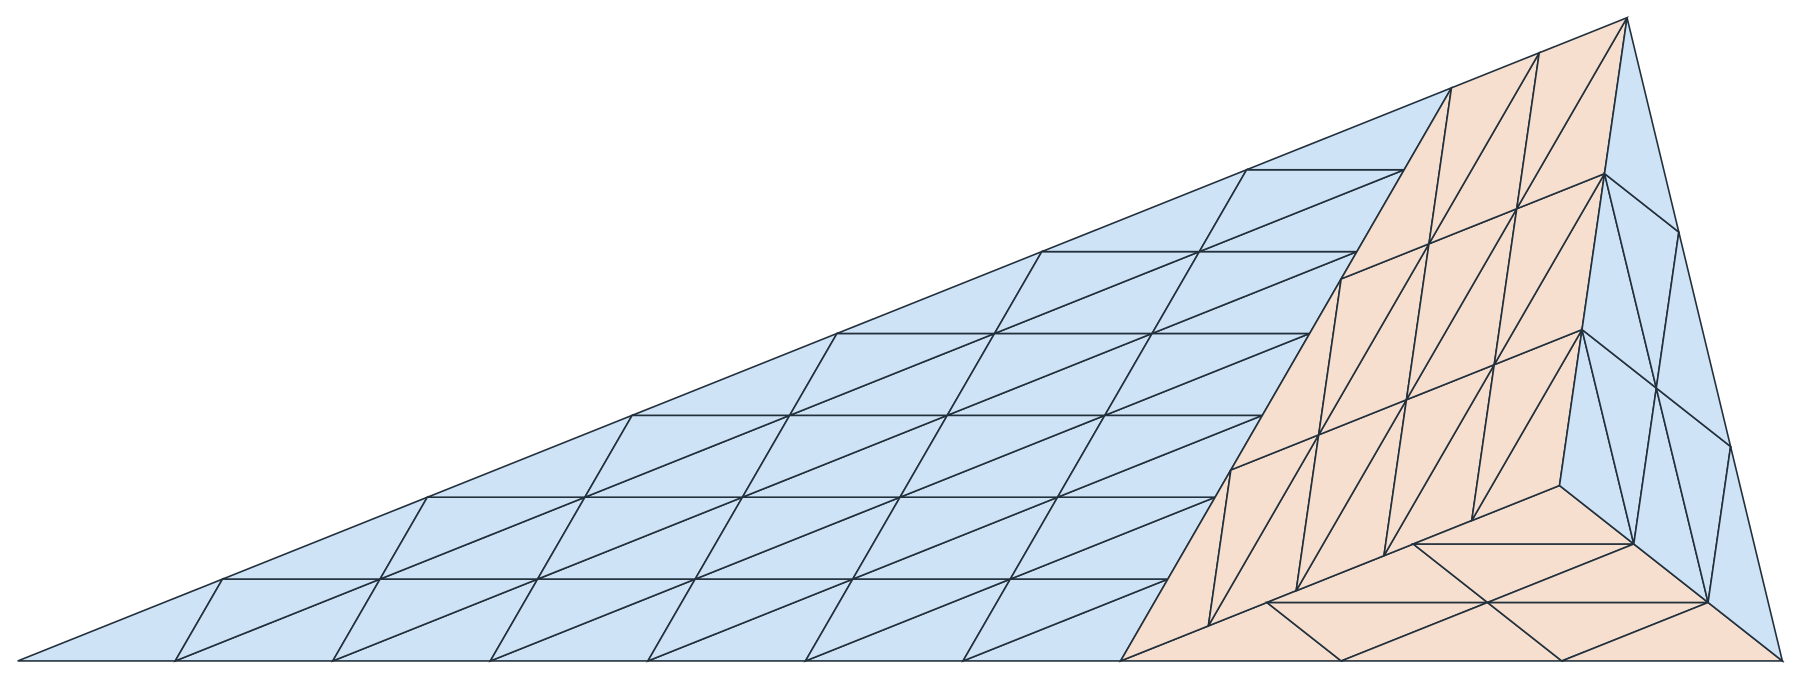
\includegraphics[width=\linewidth]{figures/N88_tiling.png}
\par\smallskip{\small $88$ copies of $(3,5,7)$ tile $(21,55,56)$.}
\end{minipage}\hfill
\begin{minipage}[t]{0.48\linewidth}
\centering
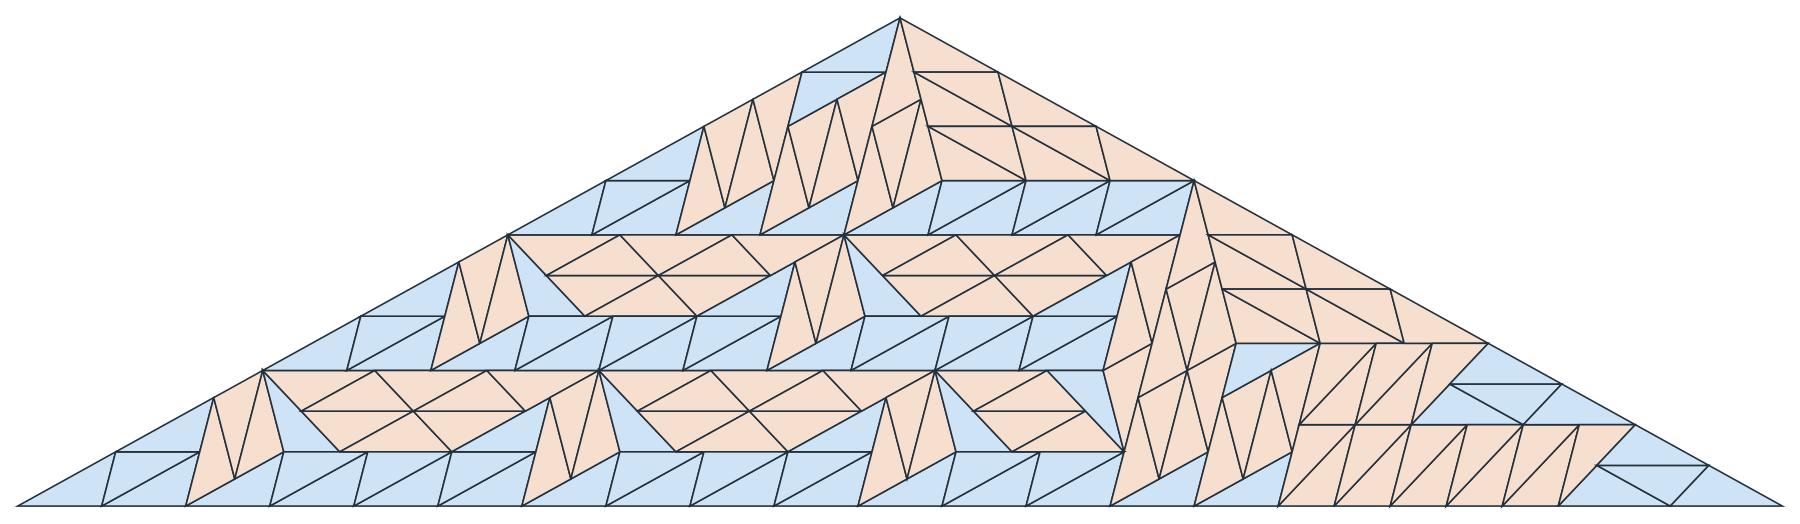
\includegraphics[width=\linewidth]{figures/N189_tiling.png}
\par\smallskip{\small $189$ copies of $(2,3,4)$ tile $(36,36,63)$.}
\end{minipage}
\caption{The two new tilings.  These images are renderings of the exact
coordinate certificates, not geometric evidence in place of them; the
certificates rendered here have SHA-256 digests beginning
\texttt{163327fc} ($N=88$) and \texttt{28f33084} ($N=189$), printed in full
in Appendix~\ref{app:positive}.}
\label{fig:newtilings}
\end{figure}

The $88$-tiling is row III of Table~\ref{tab:group2} at multiplier one:
$VW=(2a+b)(a+b)=11\cdot8=88$.  Zhang's general construction for this row,
through its published uniform threshold, first produces $7128=88\cdot9^2$
tiles for $(3,5,7)$ \cite{Zhang25}.  Thus the exact example reduces the
smallest known count on this ray by a factor $81$.

The $189$-tiling is Group~1 shape~5 for $(p,q)=(1,2)$, whose ray is
$21n^2$; see Section~\ref{sec:otherbranches}.  The known $84$- and
$336$-tilings give multipliers $2$ and $4$ \cite{Beeson2229}, while the new
tiling gives multiplier $3$.  The addition theorem below therefore yields:

\begin{corollary}[The ray $21n^2$]\label{cor:21ray}
Let the target be the Group~1 shape-5 triangle for $(p,q)=(1,2)$ at
multiplier $n$, tiled by the tile $(2,3,4)$; at $n=1$ this is the triangle
with side lengths $(12,12,21)$.
\begin{enumerate}[label=\textup{(\roman*)}]
\item \textup{(proved, from verified certificates)} For every $n\ge2$ a
      tiling exists.
\item \textup{(computer-assisted, independently certified)} For $n=1$ no
      tiling exists.
\end{enumerate}
Hence a tiling on this ray exists exactly for $n\ge2$, and
$21n^2\in\Sset$ exactly for $n\ge2$.
\end{corollary}

\begin{proof}
(i) The known $84$- and $336$-tilings give the multipliers $2$ and $4$
\cite{Beeson2229}, and Theorem~\ref{thm:88189}(ii) gives the multiplier $3$
as an exact coordinate certificate.  The corner data of
Appendix~\ref{app:addition} verify the hypotheses of
Proposition~\ref{prop:addition} for this shape, so the multiplier set is
additively closed; since $\langle2,3\rangle=\{n\ge2\}$, every $n\ge2$ occurs.

(ii) The exporter of Appendix~\ref{app:certificates}, run on this instance,
produced the refutation certificate \pathcode{N21_refutation.jsonl.gz} with
$887$ nodes and SHA-256 \texttt{70633336\ldots9eaf76}, which the independent
checker (SHA-256 \texttt{52d74ab3\ldots7fd99c}) accepts.  By
Theorem~\ref{thm:cert-sound} the target admits no tiling by $(2,3,4)$.
Corroboration, not used in the proof: the primary exact polygon search
exhausts the same instance in $415$ states with no skipped placement, a
replay with the general segment-semigroup table and boundary-invariant
pruning disabled exhausts it in $674$ states, both in the sense of
Definition~\ref{def:runstatus}; and Beeson's
Table~5 reports $n=1$ as negative on the basis of a computer boundary
search \cite{Beeson2229}.
\end{proof}

Before excluding $33$ we record the branch reduction in full.  The point of
the next proposition is that the initial list is exhaustive for a reason that
can be checked line by line against named statements of named versions,
rather than by a global appeal to a collection of classification papers.

\begin{proposition}[Complete branch reduction for $N=33$]
\label{prop:reduction33}
Let $T$ be a nondegenerate Euclidean triangle tiled by $33$ triangles
congruent to a common tile $R$; reflections are allowed and the tiling is
not assumed edge-to-edge.  Then, after possibly interchanging
$(\alpha,a)$ with $(\beta,b)$ and possibly reflecting, exactly one of the
following mutually exhaustive cases holds.
\begin{enumerate}[label=\textup{(\roman*)},leftmargin=2.6em]
\item $T$ is similar to $R$ \textup{(reptiling)}.
\item $T$ is not similar to $R$ and all three angles of $R$ are rational
      multiples of $\pi$.
\item $T$ is not similar to $R$, $\gamma=\pi/2$, and $T$ is isosceles.
\item $3\alpha+2\beta=\pi$ and $T$ has angles
      $(2\alpha,\beta,\alpha+\beta)$ \textup{(shape 1)}.
\item $3\alpha+2\beta=\pi$ and $T$ has angles $(2\alpha,\alpha,2\beta)$
      \textup{(shape 2)}.
\item $3\alpha+2\beta=\pi$ and $T$ is isosceles with base angles $\beta$,
      i.e.\ $T=(\beta,\beta,3\alpha)$ \textup{(shape 3)}.
\item $3\alpha+2\beta=\pi$ and $T$ is isosceles with base angles
      $\alpha+\beta$, i.e.\ $T=(\alpha+\beta,\alpha+\beta,\alpha)$
      \textup{(shape 4)}.
\item $3\alpha+2\beta=\pi$ and $T$ is isosceles with base angles $\alpha$,
      i.e.\ $T=(\alpha,\alpha,\alpha+2\beta)$ \textup{(shape 5)}.
\item $\gamma=2\alpha$ and $T$ is isosceles with base angles $\alpha$, i.e.\
      $T=(\alpha,\alpha,\pi-2\alpha)$.
\item $\gamma=2\pi/3$ and $T$ is isosceles with base angles $\alpha$, i.e.\
      $T=(\alpha,\alpha,\alpha+3\beta)$ \textup{(row I)}.
\item $\gamma=2\pi/3$ and $T=(\alpha,2\alpha,3\beta)$ \textup{(row II)}.
\item $\gamma=2\pi/3$ and $T=(\alpha,2\beta,2\alpha+\beta)$
      \textup{(row III)}.
\item $\gamma=2\pi/3$ and $T=(\alpha,\alpha+\beta,\alpha+2\beta)$
      \textup{(row IV)}.
\item $\gamma=2\pi/3$ and $T=(2\alpha,2\beta,\alpha+\beta)$
      \textup{(row V)}.
\item $\gamma=2\pi/3$ and $T$ is equilateral \textup{(row E)}.
\item $\gamma=\pi/3$ and $T$ is equilateral.
\end{enumerate}
In cases \textup{(iv)--(xvi)} the tile is not similar to $T$ and its angles
are incommensurable, so it may be normalized to a primitive integer triple:
to $(pq,q^2-p^2,q^2)$ with $0<p<q$, $\gcd(p,q)=1$ in cases
\textup{(iv)--(viii)} by Theorem~\ref{thm:imp-g1rat}; to
$(u^2,v^2-u^2,uv)$ with $u<v<2u$, $\gcd(u,v)=1$ in case \textup{(ix)} by
Theorem~\ref{thm:imp-g2a}; and to a solution of \eqref{eq:eisenstein} in
cases \textup{(x)--(xv)} by Theorem~\ref{thm:imp-rat}.  In case
\textup{(xvi)} the same argument applies with $c^2=a^2-ab+b^2$.

Tables~\ref{tab:disposition33} and~\ref{tab:disposition33b} dispose of every case except
\textup{(x)}, and case \textup{(x)} leaves exactly one instance: the tile
$(a,b,c)=(5,3,7)$ at scale $k=bm=3$, that is, the target with sides
$(21,21,33)$.  The eliminations use only
Lemma~\ref{lem:boundary-integrality}, Corollary~\ref{cor:rows},
Proposition~\ref{prop:group1}, Proposition~\ref{prop:gamma2alpha},
Remark~\ref{rem:boundaryscope} and the imported statements of
Section~\ref{sec:imports}.
\end{proposition}

\begin{proof}
Exhaustiveness of \textup{(i)--(xvi)}.  If $T$ is similar to $R$ we are in
case~(i).  Otherwise, if the tile angles are all rational multiples of $\pi$
we are in case~(ii).  So assume $T$ is not similar to $R$ and the tile angles
are incommensurable, and split on the shape of $T$.

If $T$ is not isosceles, Theorem~\ref{thm:imp-nonisosceles} gives shapes 1--2
of Group~1 and rows II--V of Group~2, i.e.\ cases (iv), (v) and
(xi)--(xiv).

If $T$ is isosceles and not equilateral, Theorem~\ref{thm:imp-isosceles}(i)
leaves $\gamma\in\{2\alpha,\pi/2,2\pi/3\}$ or $3\alpha+2\beta=\pi$.  The
value $\gamma=\pi/2$ is case~(iii).  Part~(iii) of that theorem restricts the
base angles of $T$ to $\alpha$, $\beta$ or $\alpha+\beta$.  For
$3\alpha+2\beta=\pi$ these three options are exactly shapes 5, 3 and 4, i.e.\
cases (viii), (vi) and (vii).  For $\gamma=2\pi/3$ one has
$\alpha+\beta=\pi/3$, so base angles $\alpha+\beta$ would make $T$
equilateral, contrary to assumption; base angles $\alpha$ or $\beta$ give
row~I, i.e.\ case (x), after the interchange $(\alpha,a)\leftrightarrow
(\beta,b)$.  For $\gamma=2\alpha$, the pairing of target shape with tile in
\cite[Table~4]{Beeson7} (Laczkovich's second table,
\cite[Thm.~4.1]{Lacz95}) is $T=(\alpha,\alpha,\pi-2\alpha)$, i.e.\ base
angles $\alpha$; this is case (ix).

If $T$ is equilateral, Theorem~\ref{thm:imp-equilateral} gives
$\gamma\in\{\pi/3,2\pi/3\}$, i.e.\ cases (xvi) and (xv).

The cases are mutually exclusive because the tile angle families
$\gamma=2\alpha$, $\gamma=\pi/2$, $\gamma=2\pi/3$, $\gamma=\pi/3$ and
$3\alpha+2\beta=\pi$ are pairwise incompatible for a tile with
incommensurable angles, and because the listed target shapes are pairwise
non-similar for such a tile.

Dispositions.  These are the entries of Tables~\ref{tab:disposition33} and~\ref{tab:disposition33b};
each is a finite arithmetic check on $N=33$, and all of them are executable
in \pathcode{computation/verify_theory_report3_claims.py}.
\end{proof}

\begin{remark}
Three hypotheses are load-bearing in the exhaustiveness argument and are
therefore stated in the proposition rather than assumed silently:
reflections are allowed, no tiling is edge-to-edge, and the case division is
by the shape of $T$ and not by the tile.  The incommensurability of the tile
angles is \emph{not} a standing hypothesis of the proposition; it is the
complement of case~(ii).  Case~(iii) is the only case in which the tile
angles may be commensurable while $T$ is not similar to $R$
\textup{(}Theorem~\ref{thm:imp-isosceles}(ii)\textup{)}, which is why the
right-tile branch is disposed of by Theorem~\ref{thm:imp-right} rather than
by an arithmetic ray.
\end{remark}

\begin{table}[ht]
\centering
\small
\renewcommand{\arraystretch}{1.15}
\begin{tabular}{@{}>{\raggedright\arraybackslash}p{0.145\linewidth}
>{\raggedright\arraybackslash}p{0.185\linewidth}
>{\raggedright\arraybackslash}p{0.375\linewidth}
>{\raggedright\arraybackslash}p{0.165\linewidth}@{}}
\toprule
branch & source theorem & $N=33$ arithmetic & disposition \\
\midrule
(i) reptile
 & Thm.~\ref{thm:imp-reptile}
 & $33$ is not a square; $33=3\cdot11$ with $11\equiv3\ (4)$ to an odd
   power, so not $e^2+f^2$; $33/3=11$ is not a square
 & excluded \\
(ii) commensurable tile
 & Thm.~\ref{thm:imp-comm}
 & $33\notin\{n^2,e^2+f^2,2n^2,3n^2,6n^2\}$: $33$ is odd, and
   $33/3=11$, $33/6\notin\Z$
 & excluded \\
(iii) right tile, $T$ isosceles
 & Thm.~\ref{thm:imp-right}
 & $33$ is odd, so $N/2\notin\Z$; $33$ is not a square; $33\ne6k^2$
 & excluded by the last clause \\
(iv) G1 shape 1
 & {\cite[Thm.~4]{Beeson2229}}; Cor.~\ref{cor:shape1ray}
 & $N=t^2(2q^2-p^2)$ with $t\in\N$; $t^2\mid33$ forces $t=1$, and
   $2q^2-p^2=33$ with $p<q$ gives $q^2<33$, i.e.\ $q\le5$, where no $p$
   solves it
 & excluded: $33$ is not of the form $t^2(2q^2-p^2)$ \\
(v) G1 shape 2
 & {\cite[Thm.~9, Table~2]{Beeson2229}}; Table~\ref{tab:group1}
 & the ray value $(2q^2-p^2)(3q^2-p^2)n^2$ is minimized at $(p,q)=(1,2)$,
   giving $7\cdot11=77>33$
 & excluded: $33$ is below the smallest shape-2 count \\
(vi) G1 shape 3
 & {\cite[Thm.~14, Cor.~2]{Beeson2229}}; Table~\ref{tab:group1}
 & the equation is $N(q+p)^2=M^2(3q^2-p^2)$, and
   $\gcd\bigl((q+p)^2,3q^2-p^2\bigr)$ forces $(q+p)\mid M$, so
   $N=u^2(3q^2-p^2)$ with $M=(q+p)u$; then $u^2\mid33$ gives $u=1$ and
   $3q^2-p^2=33$, where $2q^2<33<3q^2$ leaves only $q=4$, $p^2=15$
 & excluded: $33$ is not of the form $u^2(3q^2-p^2)$ \\
(vii) G1 shape 4
 & Prop.~\ref{prop:group1}; App.~\ref{app:rowalgebra}
 & the exact ray is $N=(q^2-p^2)m^2$; $m=1$ and $q^2-p^2=33$ give
   $(p,q)=(4,7)$ and $(16,17)$
 & excluded: $q\nmid m$ (Prop.~\ref{prop:group1}) \\
(viii) G1 shape 5
 & Prop.~\ref{prop:group1}; App.~\ref{app:rowalgebra}
 & $N=(q^2-p^2)(2q^2-p^2)n^2$; $n=1$ and the factorizations $33=1\cdot33
   =3\cdot11$ give $q^2-p^2\in\{1,3\}$, and $(p,q)=(1,2)$ has
   $2q^2-p^2=7\ne11$
 & excluded: $33$ is not on any shape-5 ray \\
(ix) $\gamma=2\alpha$
 & Prop.~\ref{prop:gamma2alpha}
 & $N=(v^2-u^2)r^2$; $r=1$ and $v^2-u^2=33$ give $(u,v)=(4,7)$ and
   $(16,17)$
 & excluded: $r\ge2$ (Prop.~\ref{prop:gamma2alpha}) \\
\bottomrule
\end{tabular}
\caption{Disposition of the branches of Proposition~\ref{prop:reduction33}
at $N=33$, part I: preliminaries, Group~1, and $\gamma=2\alpha$.  Since
$33=3\cdot11$ is squarefree, every ray equation of the form $N=Cm^2$ forces
$m=1$ and $C=33$; this is used silently in rows (iv)--(xvi) of both parts.
Rows (iv)--(vi) are stated in the strongest available form: the exclusion
uses only the tiling equation of the cited theorem and needs none of that
paper's auxiliary divisibility clauses.  Every row of both parts is an
executable check in
\pathcode{computation/verify_theory_report3_claims.py}.}
\label{tab:disposition33}
\end{table}

\begin{table}[ht]
\centering
\small
\renewcommand{\arraystretch}{1.15}
\begin{tabular}{@{}>{\raggedright\arraybackslash}p{0.145\linewidth}
>{\raggedright\arraybackslash}p{0.185\linewidth}
>{\raggedright\arraybackslash}p{0.375\linewidth}
>{\raggedright\arraybackslash}p{0.165\linewidth}@{}}
\toprule
branch & source theorem & $N=33$ arithmetic & disposition \\
\midrule
(x) G2 row I
 & Cor.~\ref{cor:rows}
 & $N=m^2bU$ with $U=a+2b$; $bU=33$ has the unique primitive solution
   $(a,b,c)=(5,3,7)$, $U=11$, at $m=1$, hence $k=bm=3$
 & \textbf{survives}: row I, $(5,3,7)$, $k=3$, target $(21,21,33)$ \\
(xi) G2 row II
 & Cor.~\ref{cor:rows}
 & $N=3m^2UW$ with $U=a+2b$, $W=a+b$; the least value of $UW$ over
   primitive triples is $11\cdot8=88$, at $(a,b)=(5,3)$, so
   $3UW\ge264>33$
 & excluded: $33$ is below the smallest row-II count \\
(xii) G2 row III
 & Cor.~\ref{cor:rows}
 & $N=m^2VW$ with $V=2a+b$; the least value of $VW$ over primitive triples
   is $11\cdot8=88>33$, at $(a,b)=(3,5)$
 & excluded: $33$ is below the smallest row-III count \\
(xiii) G2 row IV
 & Cor.~\ref{cor:rows}
 & $N=m^2bW$; the least value of $bW$ is $3\cdot8=24$, so $m=1$ and
   $bW=33$; the factorizations $(b,W)=(1,33),(3,11)$ give $a=W-b=32,8$ and
   $c^2=1057,\,97$, neither a square
 & excluded: no primitive triple has $bW=33$ \\
(xiv) G2 row V
 & Cor.~\ref{cor:rows}
 & $N=m^2UV$; the least value of $UV$ over primitive triples is
   $11\cdot13=143>33$
 & excluded: $33$ is below the smallest row-V count \\
(xv) G2 row E
 & Cor.~\ref{cor:rows} ($ab\mid L$)
 & $N=m^2ab$; $m=1$ and $ab=33$ give $(a,b)=(1,33),(3,11)$ with
   $c^2=1123,\,163$, neither a square
 & excluded: no primitive triple has $ab=33$ \\
(xvi) $\gamma=\pi/3$, $T$ equilateral
 & Rem.~\ref{rem:boundaryscope}
 & $N=m^2ab$ with $c^2=a^2-ab+b^2$; $m=1$ and $ab=33$ give
   $c^2=1057,\,97$, neither a square
 & excluded: no primitive $60^\circ$ triple has $ab=33$ \\
\bottomrule
\end{tabular}
\caption{Disposition of the branches of Proposition~\ref{prop:reduction33}
at $N=33$, part II: Group~2 and the $60^\circ$ equilateral branch.}
\label{tab:disposition33b}
\end{table}

\noindent Two independent cross-checks of the Group~1 rows are available in
the same source.  First, $33$ occurs in none of
\cite[Tables~1--5]{Beeson2229}, and each of those tables is asserted
complete to a bound exceeding $33$: shape~1 to $N\le500$
\cite[Cor.~1]{Beeson2229}, shape~2 to $N\le2000$ \cite[Table~2]{Beeson2229},
shape~3 to $N\le1000$ \cite[Cor.~2]{Beeson2229}, shape~4 to $N\le108$
\cite[Cor.~4]{Beeson2229}, and shape~5 to $N\le200$
\cite[Cor.~5]{Beeson2229}.\footnote{The range of the last of these is
printed as $N\le200$ in the statement of \cite[Cor.~5]{Beeson2229} and as
$N\le500$ in the caption of that paper's Table~5, and the corollary is
labelled ``(to Theorem 14)'' where Theorem~19 is meant.  Both bounds exceed
$33$, so the discrepancy is immaterial here.}  Second, a direct sweep of the
five tiling equations of \cite[Table~6]{Beeson2229} over
$s=p/q$ with $q\le400$ shows that shapes 1, 2, 3 and 5 admit no solution at
all with $N=33$, and that shape~4 admits only $(p,q,M)\in\{(4,7,3),(16,17,1),
(4,29,5),(29,37,2),(17,49,4)\}$, all of which fail the exact shape-4 ray
$N=(q^2-p^2)m^2$ except the first two, which fail $q\mid m$.  This sweep is
section~H of the executable audit
\pathcode{computation/verify_theory_report3_claims.py}, which also validates
the transcribed equation set against all $53$ printed rows of
\cite[Tables~1--5]{Beeson2229}.

\begin{theorem}[Computer-assisted, independently certified]\label{thm:no33}
$33\notin\Sset$.
\end{theorem}

\begin{proof}
By Proposition~\ref{prop:reduction33}, a hypothetical $33$-tiling reduces to
exactly one target: the isosceles triangle $(21,21,33)$ tiled by $(5,3,7)$,
which is row I of Table~\ref{tab:group2} at $k=3$; this agrees with Beeson's
effective isosceles enumeration \cite{BeesonIso}.

For that instance the exporter of Appendix~\ref{app:certificates} produced
the refutation certificate \pathcode{N33_refutation.jsonl.gz} with
$23157$ nodes and SHA-256 \texttt{613c52dd\ldots c21919}.  The independent checker
(SHA-256 \texttt{52d74ab3\ldots7fd99c}) accepts it in under one minute.  The checker was
written from the certificate specification alone and shares no code with the
search; the export run disables memoization and canonicalization, so the
certificate is a tree of regions in absolute coordinates, and it uses only
the three reduced pruning rules, so it depends on neither
Theorem~\ref{thm:laurent} nor the general form of
Lemma~\ref{lem:convex-segment}.  By Theorem~\ref{thm:cert-sound} the target
admits no tiling by $(5,3,7)$.

Two earlier exhaustions of the same instance corroborate this and are not
used in the proof: the primary exact polygon search exhausts it in $6479$
states with all pruning enabled, and a replay with the general
segment-semigroup table and the boundary-invariant pruning disabled returns
\texttt{EXHAUSTED} in $22850$ states.  Both runs are exhausted in the sense
of Definition~\ref{def:runstatus}, and both come from the same
implementation.
\end{proof}

\begin{remark}
The boundary invariant of Section~\ref{sec:laurent} does not exclude this
candidate: it satisfies the Laurent boundary congruence and even
admits the required exact-$N$ signed inventory.  Theorem~\ref{thm:no33} is
therefore a small but concrete demonstration that any final solution needs
interior order, incidence, or connectivity information.
\end{remark}

\section{A Laurent boundary quotient}\label{sec:laurent}

\begin{lemma}[Boundary integrality]\label{lem:boundary-integrality}
If a convex polygon is tiled by a triangle with integer side lengths, every
side of the polygon has integer length and is a concatenation of complete
tile edges.
\end{lemma}

\begin{proof}
Let $P$ be the convex polygon, $S$ one of its sides, and $\ell$ the supporting
line of $S$, so that $P$ lies in one closed half-plane bounded by $\ell$ and
\[
                          P\cap\ell=S,
\]
because the face of $P$ cut out by the supporting line of a side is that side.
Let a tile $\Delta$ meet the relative interior of $S$ in a nondegenerate
segment.  Then $\ell$ supports $\Delta$ as well, so $\Delta\cap\ell$ is a face
of $\Delta$; it has positive dimension, hence is a complete edge of $\Delta$.
Moreover $\Delta\cap\ell\subseteq P\cap\ell=S$, so that edge cannot extend
beyond either endpoint of $S$.  Distinct such edges have disjoint relative
interiors.  Every point of $S$ lies in some tile; a tile that does not
contribute one of the edges just described meets $\ell$ in at most one point,
and there are finitely many tiles, so those edges cover $S$ up to a finite
set.  Their union is closed, hence equals $S$, and their integer lengths add to
the length of $S$.  No edge-to-edge hypothesis is used.
\end{proof}

In a Group~2 tiling, every directed edge direction has a unique expression
\[
             \theta=j\pi/3+m\alpha,\qquad j\in\Z/6,\quad m\in\Z,
\]
after an anchor is chosen; here $\alpha/\pi$ is irrational
\cite{BZRat}.  Put $d=a-b$ and define the character
\[
       \chi(j,m)=(-1)^jz^m\in\Z[z,z^{-1}]^\times.
\]
The pair $(j,m)$ is determined by $\theta$.  Indeed, if
$j\pi/3+m\alpha\equiv j'\pi/3+m'\alpha\pmod{2\pi}$, then
$(m-m')\alpha\in\pi\Q$, so $m=m'$ because $\alpha/\pi$ is irrational, and then
$(j-j')\pi/3\in2\pi\Z$ gives $j\equiv j'\pmod6$.  The irrationality used here
is proved in Appendix~\ref{app:ordered}: $2\cos\alpha=U/c$ is rational and
lies strictly between $1$ and $2$, so it is not a rational integer, whereas
$\alpha/\pi\in\Q$ would force it to be one; see also \cite{BZRat}.  We
therefore write $\chi(\theta)$ for $\chi(j,m)$.

For a directed segment $PQ$ of direction $\theta$, set
$B(PQ)=|PQ|\chi(\theta)$, initially in
$\mathbb R[z,z^{-1}]$, and extend $B$ additively to oriented polygonal
chains.  By Lemma~\ref{lem:boundary-integrality}, complete tile and target
boundaries have integral coefficients.

\begin{theorem}[Laurent boundary quotient]\label{thm:laurent}
Let a triangle be tiled by a primitive Group~2 tile satisfying
\eqref{eq:eisenstein}, and write $R=\Z[z,z^{-1}]$ and
$\pi_I:R\to R/I$ for the quotient map.  Then
\begin{equation}\label{eq:ideal}
       B(\partial T)\in I=(d+cz,\ d+cz^{-1})\subseteq R,
\end{equation}
and $3ab\in I$.  Moreover the following two maps are mutually inverse ring
isomorphisms:
\begin{equation}\label{eq:quotient}
\begin{aligned}
 \overline\varepsilon&:R/I\longrightarrow\Z/(3ab),
  &&\text{induced by }\ \varepsilon:R\to\Z/(3ab),\quad z\longmapsto-dc^{-1},\\
 \overline\iota&:\Z/(3ab)\longrightarrow R/I,
  &&\text{induced by }\ \Z\hookrightarrow R\xrightarrow{\ \pi_I\ }R/I .
\end{aligned}
\end{equation}
Here $\varepsilon$ is well defined because $c$ and $d$ are units modulo $3ab$
(Lemma~\ref{lem:g2-units}), and $\overline\iota$ is well defined because
$I\cap\Z=(3ab)$.  Consequently \eqref{eq:ideal} is equivalent to the single
evaluation
\begin{equation}\label{eq:eval}
       B(\partial T)\big|_{z=-dc^{-1}}\equiv0\pmod{3ab}.
\end{equation}
\end{theorem}

\begin{proof}
The counterclockwise boundary of a direct tile, with its $a$-edge anchored,
has value
\[
                    d+cz^{-1};
\]
a reflected tile has value $d+cz$, up to multiplication by a Laurent unit.
Subdivide every tile edge at every tiling vertex.  In this common refinement,
each elementary interior segment is incident with exactly one tile on each
side, so it occurs twice with opposite orientations and cancels.  This proves
\eqref{eq:ideal}; no edge-to-edge hypothesis is being imposed.

Since $c^2-d^2=3ab$,
\begin{equation}\label{eq:3ab-in-I}
 c(d+cz)-dz(d+cz^{-1})=(c^2-d^2)z=3abz,
\end{equation}
and $z$ is a unit of $R$, so $3ab\in I$.

By Lemma~\ref{lem:g2-units} the residues of $c$ and $d$ are units modulo
$3ab$, so $-dc^{-1}$ is a unit there and $\varepsilon$ is a well-defined ring
homomorphism.  It kills both generators of $I$:
\[
 \varepsilon(d+cz)=d-c\,dc^{-1}=0,\qquad
 \varepsilon(d+cz^{-1})=d-c^2d^{-1}=-3ab\,d^{-1}=0 .
\]
Hence $I\subseteq\ker\varepsilon$ and $\varepsilon$ induces
$\overline\varepsilon$ on $R/I$.

For the other direction, work in $R/I$.  By \eqref{eq:3ab-in-I} we have
$3ab=0$ there, and $\gcd(c,3ab)=1$ gives integers $c',n$ with $cc'=1+3abn$,
so $c'$ inverts $c$ in $R/I$.  The two generators of $I$ therefore give
\[
             z=-c'd,\qquad z^{-1}=-c'd
\]
in $R/I$, so every Laurent monomial is congruent there to an integer and
$\Z\hookrightarrow R\xrightarrow{\pi_I}R/I$ is surjective.  Its
kernel is $I\cap\Z$, and
\[
 (3ab)\subseteq I\cap\Z\subseteq\ker\varepsilon\cap\Z=(3ab),
\]
the first inclusion by \eqref{eq:3ab-in-I} and the last because
$\varepsilon$ restricted to $\Z$ is reduction modulo $3ab$.  Hence
$I\cap\Z=(3ab)$ and $\overline\iota$ is a well-defined ring isomorphism.
Finally $\overline\varepsilon\circ\overline\iota$ is the identity of
$\Z/(3ab)$, again because $\varepsilon|_\Z$ is reduction modulo $3ab$;
as both maps are bijections, $\overline\iota$ and $\overline\varepsilon$ are
mutually inverse.  This proves \eqref{eq:quotient}, and $\ker\varepsilon=I$
gives the equivalence of \eqref{eq:ideal} with \eqref{eq:eval}.
\end{proof}

\begin{corollary}[Universal property of the boundary quotient]
\label{cor:laurent-universal}
Let $A$ be a commutative ring and let $\phi:\Z[z,z^{-1}]\to A$ be a ring
homomorphism with
\[
             \phi(d+cz)=\phi(d+cz^{-1})=0 .
\]
Then there is a unique ring homomorphism $\psi:\Z/(3ab)\to A$ with
$\phi=\psi\circ\varepsilon$.  In particular $3ab\cdot1_A=0$, the element
$\phi(c)$ is invertible in $A$, and $\phi(z)=-\phi(d)\phi(c)^{-1}$.
Consequently, for every tiling as in Theorem~\ref{thm:laurent},
\[
 \phi\big(B(\partial T)\big)
 =\psi\Big(B(\partial T)\big|_{z=-dc^{-1}}\Big),
\]
so every boundary invariant obtained by specializing the character $\chi$
along such a $\phi$ factors through the cyclic quotient
\eqref{eq:quotient}, and no such specialization can obstruct a candidate that
satisfies \eqref{eq:eval}.
\end{corollary}

\begin{proof}
The hypotheses give $I\subseteq\ker\phi$, and $\ker\varepsilon=I$ by
Theorem~\ref{thm:laurent}, so $\phi$ factors as $\psi\circ\varepsilon$; the
factor $\psi$ is unique because $\varepsilon$ is surjective.  Then
$3ab\cdot1_A=\phi(3ab)=\psi(0)=0$, and $\phi(c)=\psi(\varepsilon(c))$ is
invertible because $\varepsilon(c)$ is a unit of $\Z/(3ab)$ by
Lemma~\ref{lem:g2-units}, whence
$\phi(z)=-\phi(c)^{-1}\phi(d)$ from $\phi(d+cz)=0$.  Applying $\psi$ to
$\varepsilon(B(\partial T))$ gives the displayed identity, and the last
assertion is that identity read backwards: if \eqref{eq:eval} holds, the
argument of $\psi$ vanishes.
\end{proof}

\begin{remark}[Scope of Corollary~\ref{cor:laurent-universal}]
\label{rem:laurent-scope}
Signed characters, root-of-unity specializations, and reductions modulo a
divisor of $3ab$ all satisfy the hypothesis of
Corollary~\ref{cor:laurent-universal} and are therefore already contained in
\eqref{eq:eval}.  The corollary says nothing about invariants that are not
ring specializations of $\chi$: bounds on the number or on the signs of the
$N$ admissible tile terms representing $B(\partial T)$, and any use of edge
order, incidence, or connectivity, lie outside its scope.  This is what
Theorem~\ref{thm:no33} exhibits concretely.
\end{remark}

\begin{corollary}[Exact Group~2 arithmetic]\label{cor:rows}
The six necessary conditions and count rays in
Table~\ref{tab:group2} hold for every Group~2 tiling.
\end{corollary}

\begin{proof}
Evaluate the counterclockwise target boundary in
\eqref{eq:eval}.  Up to multiplication by units modulo $3ab$, the six
residues are
\[
\begin{array}{c|cccccc}
\text{row}&\mathrm{I}&\mathrm{II}&\mathrm{III}&\mathrm{IV}&\mathrm{V}&\mathrm{E}\\
\hline
B(\partial T)&3a^2k&0&0&3ak&0&3L.
\end{array}
\]
Since $\gcd(a,b)=1$, the nonzero entries give $b\mid k$ in rows I and IV
and $ab\mid L$ in row E.  The area equations give the counts in
Table~\ref{tab:group2}.  The primitive target side vectors make the remaining
scale integral; detailed row polynomials and gcd checks are recorded in
Appendix~\ref{app:rowalgebra}.
\end{proof}

\begin{remark}[What the invariant closes]\label{rem:boundaryscope}
The quotient proves Zhang's divisibility conjecture for equilateral
$120^\circ$ tiles, including the nonsquarefree cases not covered by his
lemma.  It also removes the congruence hypothesis from Zhang's row-V count
formula \cite{Zhang25}.  The same proof works for $60^\circ$ tiles after
replacing $c^2=a^2+ab+b^2$ by $c^2=a^2-ab+b^2$ and $d=a-b$ by $d=a+b$: the
one-tile polynomials become, up to units, $d-cz^{-1}$ and $d-cz$, while
$c^2-d^2=-3ab$, so that
\[
 c(d-cz)+dz(d-cz^{-1})=(d^2-c^2)z=3abz,
\]
and Lemma~\ref{lem:g60-units} supplies exactly the units the argument of
Theorem~\ref{thm:laurent} consumes: $c$ and $d=a+b$ are invertible modulo
$3ab$.  The evaluation is $z\mapsto dc^{-1}$ and the quotient is again
$\Z/(3ab)$.  Conversely, by Corollary~\ref{cor:laurent-universal} all
ideal-membership obstructions obtained by specializing this Laurent character
are exhausted; the invariants excluded from that statement are listed in
Remark~\ref{rem:laurent-scope}.
\end{remark}

\section{Construction thresholds and additive multiplier sets}
\label{sec:semigroup}

For $x,L>0$, an \emph{ideal trapezoid} $T(x,L)$ has parallel sides $x$ and $x+L$, base
angles $\pi/3$, and two legs of length $L$.\footnote{Zhang
\cite{Zhang25} interchanges the leg and long-side symbols; here $L$ is the leg.}
Its Laurent boundary is $3L$,
independent of $x$, so Theorem~\ref{thm:laurent} gives the necessary condition
$ab\mid L$.

The construction below uses two statements of \cite{Zhang25} verbatim, both
read with $y$ meaning the leg, as that paper's own proofs do.

\begin{lemma}[Imported; basic ideal trapezoid, {\cite[Lemma~1]{Zhang25}}]
\label{lem:imp-zhang1}
The ideal trapezoid with short parallel side $x=a^2+b^2$ and leg $L=ab$ is
tiled by $(a,b,c)$; it splits into the three triangles similar to $(a,b,c)$
with integer factors $a$, $b$, $c$, hence into $a^2+b^2+c^2$ tiles.
\end{lemma}

\begin{lemma}[Imported; parallelograms, {\cite[Lemma~2]{Zhang25}}]
\label{lem:imp-zhang2}
A parallelogram whose angles are, in order, $2\pi/3$, $\pi/3$, $2\pi/3$,
$\pi/3$, and whose side lengths are $x$ and $ab$, is tiled by $(a,b,c)$
whenever $x>ab-a-b$.  The proof glues two
tiles along $c$ into an $(a,b,a,b)$ parallelogram, forms the
$(ab,a,ab,a)$ and $(ab,b,ab,b)$ parallelograms from it in the two
orientations, and concatenates them; it therefore proves the sharper
statement that the parallelogram is tiled whenever
$x\in a\Nzero+b\Nzero$.
\end{lemma}

\noindent The sharper reading of Lemma~\ref{lem:imp-zhang2} is what
Lemma~\ref{lem:trapezoid} uses; the Frobenius bound $x>ab-a-b$ of
\cite[Prop.~2]{Zhang25} is only the crude sufficient condition for
$x\in a\Nzero+b\Nzero$.

\begin{lemma}[Trapezoid construction]\label{lem:trapezoid}
Let $R=(a,b,c)$ be a primitive $120^\circ$ tile.  If
\[
       x,L\in\N,\qquad
       ab\mid L,\qquad x-(a^2+b^2)\in a\Nzero+b\Nzero,
\]
then $T(x,L)$ is tiled by
\[
                    \frac{L(2x+L)}{ab}
\]
copies of $R$.
\end{lemma}

\begin{proof}
Lemma~\ref{lem:imp-zhang1} supplies the basic trapezoid $T(a^2+b^2,ab)$ and
Lemma~\ref{lem:imp-zhang2} the
$\pi/3$-parallelograms of side $ab$ and base $a$ or $b$.
Write $L=kab$ and slice $T(x,L)$ into $k$
layers of leg $ab$.  In layer $i$, remove a copy of the basic trapezoid.
The remainder is a parallelogram whose base is
\[
       x+(i-1)ab-(a^2+b^2)\in a\Nzero+b\Nzero,
\]
so it is tiled by concatenating the two parallelograms of
Lemma~\ref{lem:imp-zhang2}.  The area ratio
gives the stated number of tiles.
\end{proof}

For $x=rab$, the semigroup condition in Lemma~\ref{lem:trapezoid} is
equivalent to
\[
 r\ge R(a,b):=\left\lceil\frac ab\right\rceil+
              \left\lceil\frac ba\right\rceil.
\]
Indeed, if $rab-a^2-b^2=Aa+Bb$, reduction modulo $b$ and $a$ gives
$A=ub-a$ and $B=va-b$ for integers
$u\ge\lceil a/b\rceil$, $v\ge\lceil b/a\rceil$, and then $r=u+v$.
The converse follows from the same formulae.  In the cyclic equilateral
construction of Theorem~\ref{thm:imp-zhang4} below, which assembles an
equilateral triangle of side $(r+s+t)ab$ from three ideal trapezoids with
parameters $r,s,t$, choose the parameters
$R,R,m-2R$; Lemma~\ref{lem:trapezoid} tiles each of the three trapezoids
because all parameters are at least $R$, exactly when $m\ge3R$.  This gives
an equilateral tiling for every such multiplier.  At
$(a,b,c)=(32,45,67)$ this gives the smaller multiplier
$m=9$.\footnote{The threshold printed in \cite[Conjecture~2]{Zhang25} is
$12$, so that conjectured threshold is not sharp.}  The count $116640$ is
already classical, so this changes the construction theory rather than
$\Sset$ itself.

\begin{proposition}[Multiplier addition]\label{prop:addition}
Let $\Delta$ be a triangle and $R$ a tile.  Suppose one vertex of $\Delta$
has adjacent sides $L_1,L_2$, while two adjacent sides $e_1,e_2$ of $R$
meet at that angle or its supplement, and
$L_1/e_1,L_2/e_2\in\N$.  If $r,s\in\N$ and $r\Delta$ and $s\Delta$ are
tiled by $R$, then
$(r+s)\Delta$ is tiled by $R$.
\end{proposition}

\begin{proof}
Write $\Delta=\operatorname{conv}(O,A,B)$.  In $(r+s)\Delta$, put
$P=rA$, $Q=rB$, and $D=rA+sB$.  The three regions
\[
 \triangle OPQ,\qquad P+s\Delta,\qquad
 \operatorname{conv}(P,Q,(r+s)B,D)
\]
have disjoint interiors and fill $(r+s)\Delta$; the last is a
parallelogram with side lengths $r|B-A|$ and $s|B|$.  Labeling the chosen
corner of $\Delta$ as $B$ makes these $rL_1$ and $sL_2$.
Subdivide the parallelogram into an
$r(L_1/e_1)$ by $s(L_2/e_2)$ grid of parallelograms with sides
$e_1,e_2$, and split every cell along the diagonal determined by whether
the included angle is the tile angle or its supplement.  The two halves are
congruent copies of $R$ by SAS.  No edge-to-edge hypothesis is used.
\end{proof}

For a fixed ray, let $\Aset$ be the set of positive multipliers that admit
a tiling.  Here a \emph{numerical semigroup} means a cofinite additive
submonoid of $\Nzero$.  The hypotheses of Proposition~\ref{prop:addition} hold on all
six Group~2 rows and on Group~1 shapes 4 and 5; the integer ratios are given
in Appendix~\ref{app:addition}.

The transfer of an equilateral tail to the other rows is imported.  Call
$L$ \emph{equiconstructible} for $(a,b,c)$ if the equilateral triangle of
side $L$ is tiled by $(a,b,c)$.

\begin{theorem}[Imported; equilateral construction,
{\cite[Thm.~4]{Zhang25}}]\label{thm:imp-zhang4}
Put $M_Z=3\lceil(c^2-a-b)/(ab)\rceil$.  Then $mab$ is equiconstructible for
every integer $m\ge M_Z$, and hence an $m^2ab$-tiling exists for every such
$m$.  The proof assembles an equilateral triangle of side $(r+s+t)ab$ from
three ideal trapezoids with parameters $r,s,t\ge M_Z$.
\end{theorem}

\begin{proposition}[Imported; row transfers from an equilateral core,
{\cite[Props.~8--10]{Zhang25}}]\label{prop:imp-zhang810}
Suppose $mab$ is equiconstructible for $(a,b,c)$.  Then, in the notation of
Table~\ref{tab:group2},
\begin{enumerate}[label=\textup{(\alph*)}]
\item \textup{\cite[Prop.~8(1)]{Zhang25}} the triangle
      $(mbc,mbc,mb(a+2b))$, of shape row~I with $k=bm$, is tiled by
      $m^2b(a+2b)$ copies of $(a,b,c)$;
\item \textup{\cite[Prop.~9(1)]{Zhang25}} the triangle
      $(mab,mbc,mb(a+b))$, of shape row~IV with $k=bm$, is tiled by
      $m^2b(a+b)$ copies;
\item \textup{\cite[Prop.~10(1)]{Zhang25}} the triangle
      $\bigl(mac,(b+2a)mb,(a+b)cm\bigr)$, of shape row~III with $k=m$, is
      tiled by $m^2(b+2a)(a+b)$ copies.
\end{enumerate}
In each case the statement with $a$ and $b$ interchanged also holds.
\end{proposition}

\begin{proposition}[Imported; row-V to row-II transfer,
{\cite[Prop.~11]{Zhang25}}]\label{prop:imp-zhang11}
If the triangle $\bigl((a+2b)am,(b+2a)bm,c^2m\bigr)$---row~V at multiplier
$m$---is tiled by $(a,b,c)$, then the triangle
$\bigl(c^2m,(a+2b)mc,3(a+b)mb\bigr)$---row~II at multiplier $m$---is tiled by
$3m^2(a+2b)(a+b)$ copies of $(a,b,c)$, and likewise with $a$ and $b$
interchanged.
\end{proposition}

\noindent Propositions~\ref{prop:imp-zhang810} and~\ref{prop:imp-zhang11}
are used only as implications: (a)--(c) consume only equiconstructibility of
$mab$, supplied here by the tail $m\ge3R(a,b)$ proved above, and
Proposition~\ref{prop:imp-zhang11} consumes the row-V interval produced by
the bisector dissection of Appendix~\ref{app:addition}.

\pagebreak[3]
\begin{corollary}[Finite generator windows]\label{cor:windows}
For every primitive Group~2 tile and every row of
Table~\ref{tab:group2}, $\Aset\cup\{0\}$ is a numerical semigroup.
More precisely:
\begin{enumerate}[label=\textup{(\roman*)}]
\item in rows E, I, III, and IV, every $m\ge3R(a,b)$ occurs and
\[
 \Aset\cup\{0\}
 =\big\langle\Aset\cap[1,6R(a,b)-1]\big\rangle;
\]
\item in rows V and II, every $s\ge\lceil3R(a,b)/2\rceil$ occurs and
\[
 \Aset\cup\{0\}
 =\big\langle\Aset\cap
 [1,2\lceil3R(a,b)/2\rceil-1]\big\rangle.
\]
\end{enumerate}
Thus each Group~2 ray is determined by finitely many exact tiling questions.
\end{corollary}

\begin{proof}
Additive closure is Proposition~\ref{prop:addition}.  The equilateral tail
$m\ge3R(a,b)$ was proved immediately above from
Lemma~\ref{lem:trapezoid} and the cyclic construction of
Theorem~\ref{thm:imp-zhang4}.
Proposition~\ref{prop:imp-zhang810}(a)--(c) transfers that tail to rows I,
IV, and III.  For rows V and II,
a bisector dissection transfers an equilateral tiling of side $2sab$ to row V
at multiplier $s$; the dissection and count identity are in
Appendix~\ref{app:addition}.  Proposition~\ref{prop:imp-zhang11} transfers
the same interval to row II.
Finally, if an additively closed set contains every integer at least $C$,
then each $n\ge2C$ is $C+(n-C)$ and induction shows that the set is generated
by its members below $2C$.  The complement is finite, so
$\Aset\cup\{0\}$ is a numerical semigroup.
\end{proof}

\begin{theorem}[Trapezoid tilings for $(3,5,7)$: the constructive half]
\label{thm:trapezoid-plus}
For the tile $(3,5,7)$ and $L=15$, the ideal trapezoid $T(x,15)$ is tiled by
$(3,5,7)$ for every integer $x\in\{29,31,32\}$ and every integer $x\ge34$.
\end{theorem}

\begin{proof}
Here $ab=15=L$, so Lemma~\ref{lem:trapezoid} applies whenever
$x-34\in3\Nzero+5\Nzero$, that is for $x=34,37,39,40$ and every $x\ge42$.
The seven exact coordinate certificates listed in
Appendix~\ref{app:trapezoids} cover
\[
  x=29,\ 31,\ 32,\ 35,\ 36,\ 38,\ 41 .
\]
Each passes the checks of Appendix~\ref{app:positive}, including the
trapezoid-shape assertions, so by Lemma~\ref{lem:coverage} its tiles cover
the intended trapezoid exactly.
\end{proof}

\begin{theorem}[Trapezoid tilings for $(3,5,7)$: the exclusion half;
computer-assisted]\label{thm:trapezoid-minus}
For the tile $(3,5,7)$, $L=15$, and every integer $x$ with $1\le x\le33$ and
$x\notin\{29,31,32\}$, the ideal trapezoid $T(x,15)$ admits no tiling by
$(3,5,7)$.
\end{theorem}

\begin{proof}
The boundary inventory excludes every positive $x\notin\langle3,5,7\rangle$,
namely $x\in\{1,2,4\}$.  For the remaining values the exact searcher was
run; the search found precisely the $27$ exhausted cases
\[
 \langle3,5,7\rangle\cap[1,33]\setminus\{29,31,32\},
\]
each terminating with status exhausted in the sense of
Definition~\ref{def:runstatus}, with no skipped placement and no unsupported
geometric case.  Completeness of each search tree is
Lemmas~\ref{lem:corner-branching}, \ref{lem:flush-list}, \ref{lem:fit},
\ref{lem:exact-subtraction} and~\ref{lem:components}, and every prune used
is one of the necessary conditions of Lemma~\ref{lem:prunes}.  The campaign
comprises $34$ searches and $5{,}699{,}235$ states;
Appendix~\ref{app:trapezoids} gives the case table and the completeness
scope.
\end{proof}

\noindent
This half depends on a single exhaustion implementation: no refutation
certificate has been exported for these instances.  The pipeline of
Appendix~\ref{app:certificates} applies to trapezoid targets without change,
and the deferred campaign, with the commands it needs, is recorded with the
certificate specification in the ancillary files.

\begin{corollary}[The one-leg family at $L=15$]\label{cor:trapezoid357}
For the tile $(3,5,7)$, $L=15$, and every integer $x\ge1$,
\[
 T(x,15)\text{ is tileable}
 \quad\Longleftrightarrow\quad
 x\in\{29,31,32\}\cup\{x\in\N:x\ge34\}.
\]
The implication ``$\Leftarrow$'' is Theorem~\ref{thm:trapezoid-plus} and is
proved.  The implication ``$\Rightarrow$'' is
Theorem~\ref{thm:trapezoid-minus} and therefore carries that theorem's
evidence class: computer-assisted, one implementation, no independent
certificate.
\end{corollary}

Corollary~\ref{cor:trapezoid357} gives the complete local picture for this
one-leg family, with its two evidence classes separated by
Theorems~\ref{thm:trapezoid-plus} and~\ref{thm:trapezoid-minus}.\footnote{The
literal inequality in \cite[Conjecture~5]{Zhang25} does not hold as printed
and already conflicts with the basic construction in
\cite[Lemma~1]{Zhang25}.}  The necessary divisibility $ab\mid L$ remains
valid.

\section{The remaining arithmetic branches}\label{sec:otherbranches}

For Group~1, normalize $a/c=p/q$ with $0<p<q$ and $\gcd(p,q)=1$.  A primitive
tile has sides
\[
                  (pq,\ q^2-p^2,\ q^2).
\]
The five target shapes lie on the rays in Table~\ref{tab:group1}.  Shapes
1--3 are characterized by Beeson \cite{Beeson2229}.  Shapes 4--5 are
necessity statements; their sufficiency remains open in general.

The shape-1 count is used below, so we state it in the present
normalization.  Beeson's shape-1 analysis is carried by two statements.

\begin{theorem}[Imported; shape-1 necessity,
{\cite[Thm.~4]{Beeson2229}}]\label{thm:imp-b4}
Let $3\alpha+2\beta=\pi$ and let $T$ have angles
$(2\alpha,\beta,\alpha+\beta)$ and be $N$-tiled by a tile with angles
$\alpha$ and $\beta$.  Then $M^2+N=2K^2$ for some positive integers $M,K$
with $M^2<N$, where $s=2\sin(\alpha/2)=M/K$; and $N$ is a square times a
product of distinct primes of the form $8n\pm1$.
\end{theorem}

\begin{theorem}[Imported; shape-1 divisibility,
{\cite[Thm.~6]{Beeson2229}}]\label{thm:imp-b6}
Let $T$ have angles $(2\alpha,\beta,\alpha+\beta)$, let integers $N,K,M$
solve $N=2K^2-M^2$, and suppose there is an $N$-tiling of $T$ by a tile with
angles $(\alpha,\beta,\gamma)$ and sides $(a,b,c)$ with $a/c=M/K$.  Then
$K\mid M^2$.
\end{theorem}

\begin{corollary}[Shape-1 ray]\label{cor:shape1ray}
With the normalization $a/c=p/q$ of this section, the count of every
shape-1 tiling is
\[
   N=q^2(2q^2-p^2)n^2,\qquad n\in\N,
\]
and conversely every such $N$ occurs \textup{(\cite[Thm.~5]{Beeson2229})}.
\end{corollary}

\begin{proof}
By Lemma~2 of \cite{Beeson2229}, $s=2\sin(\alpha/2)=a/c=p/q$.  Let $(M,K)$
be as in Theorem~\ref{thm:imp-b4}.  From $M/K=p/q$ with $\gcd(p,q)=1$ we get
$M=pt$, $K=qt$ for an integer $t\ge1$, whence
$N=2K^2-M^2=t^2(2q^2-p^2)$.  Theorem~\ref{thm:imp-b6} applies to this
$(M,K)$ and gives $qt\mid p^2t^2$, i.e.\ $q\mid p^2t$, i.e.\ $q\mid t$.
Writing $t=qn$ gives the displayed ray.  Conversely, for $(M,K)=(pqn,q^2n)$
one has $M^2+N=2q^4n^2=2K^2$, $M^2<N$ and $K\mid N$, so
\cite[Thm.~5]{Beeson2229} produces an $N$-tiling, by the tile
$n\cdot(pq,q^2-p^2,q^2)$.
\end{proof}

\noindent Only Corollary~\ref{cor:shape1ray} is used later, in the proof of
Proposition~\ref{prop:group1}.  We do not use the printed statement
\cite[Thm.~7]{Beeson2229}, which asserts the existence of an $N$-tiling if
and only if the tiling equation has a solution with $K\nmid M^2$; that
inequality contradicts Theorems~5 and~6 of the same paper and the proof of
Theorem~7 itself, and is a typographical negation.

\begin{proposition}\label{prop:group1}
For every Group~1 shape-4 tiling, the natural multiplier $m$ satisfies
$q\mid m$; hence its count has the shape-4 form in
Table~\ref{tab:group1}.  Every shape-5 tiling has the shape-5 count in that
table, without an additional parity factor.  The multiplier sets for shapes
4 and 5, with zero adjoined, are additive submonoids of $\Nzero$.
\end{proposition}

\begin{proof}
For shape 4, an exact target insertion gives equal side
$X=(q^2-p^2)qm$.  Attach a $qm$-scaled tile along that side.  The union is a
shape-1 target with count $(2q^2-p^2)m^2$.  Corollary~\ref{cor:shape1ray}
says its count is
$q^2(2q^2-p^2)n^2$, forcing $m=qn$.
For shape 5, cancellation in the Group~1 boundary ideal forces the target
scale $C$ to be divisible by $q^2-p^2$, giving the listed count.  The
factorization and target insertion are recorded in
Appendix~\ref{app:rowalgebra}.  Additive closure is
Proposition~\ref{prop:addition}.
\end{proof}

Unlike Corollary~\ref{cor:windows}, this proposition supplies neither a tail
nor an a priori finite generator window for shapes 4 and 5.

\begin{table}[ht]
\centering
\small
\renewcommand{\arraystretch}{1.12}
\begin{tabular}{@{}c>{\raggedright\arraybackslash}p{0.36\linewidth}
>{\raggedright\arraybackslash}p{0.45\linewidth}@{}}
\toprule
shape & target angles & necessary count ray \\
\midrule
1 & $(2\alpha,\beta,\alpha+\beta)$
  & $q^2(2q^2-p^2)n^2$ \\
2 & $(2\alpha,\alpha,2\beta)$
  & $(2q^2-p^2)(3q^2-p^2)n^2$ \\
3 & $(\beta,\beta,3\alpha)$
  & $q^2(3q^2-p^2)n^2$ \\
4 & $(\alpha+\beta,\alpha+\beta,\alpha)$
  & $q^2(q^2-p^2)n^2$ \\
5 & $(\alpha,\alpha,\alpha+2\beta)$
  & $(q^2-p^2)(2q^2-p^2)n^2$ \\
\bottomrule
\end{tabular}
\caption{Group~1 rays.  In shape 4 the natural scale $m$ is divisible by
$q$, so $m=qn$; in shape 5 there is no additional parity factor, including
when $p$ and $q$ are both odd.}\label{tab:group1}
\end{table}

\begin{remark}[Erratum: the clause $g\mid M$ of {\cite[Thm.~19]{Beeson2229}}]
\label{rem:gM}
Proposition~\ref{prop:group1} deliberately does not use a further
divisibility clause carried by the published shape-5 necessity theorem.  We
record why, because a reader who imports that clause will exclude values
that are not excluded.

\emph{The cited statement.}  \cite[Thm.~19]{Beeson2229} reads, verbatim:
``Suppose $3\alpha+2\beta=\pi$.  Let $ABC$ be isosceles with base angles
$\alpha$.  Suppose $ABC$ is $N$-tiled by the tile whose integer sides
$(a,b,c)$ have no common factor, and whose angles are
$(\alpha,\beta,\gamma)$.  Let $s=a/c$ and $g=\gcd(a,c)$, and let $M$ be the
coloring number of the tiling.  Then $g$ divides $M$, $M^2\le2N$, and
$(M,s)$ is a solution of the `isosceles-$\alpha$ tiling equation'
\[
   N=M^2\frac{(1+s)(2-s^2)}{(1-s)(2+s)^2}\text{.''}
\]

\emph{Translation of notation.}  In the normalization of this section the
tile is $(a,b,c)=(pq,\,q^2-p^2,\,q^2)$, so
\[
   s=\frac ac=\frac pq,\qquad g=\gcd(pq,q^2)=q .
\]
Beeson's $M$ is the coloring number of the tiling, not our multiplier $n$.
Substituting $s=p/q$ in the displayed equation gives
\[
   \frac{N}{M^2}=\frac{(q+p)(2q^2-p^2)}{(q-p)(2q+p)^2},
\]
and combining this with the shape-5 ray $N=(q^2-p^2)(2q^2-p^2)n^2$ of
Proposition~\ref{prop:group1} yields
\[
   M=(q-p)(2q+p)\,n .
\]
Hence, on the ray, the printed clause is equivalent to a statement about our
own multiplier:
\[
  g\mid M
  \iff q\mid(q-p)(2q+p)n
  \iff q\mid p^2n
  \iff q\mid n ,
\]
the last step by $\gcd(p,q)=1$.

\emph{A counterexample.}  Take $(p,q)=(1,2)$, tile $(2,3,4)$, and $n=3$.
Then $s=1/2$, $g=2$, and
\[
   \frac{N}{M^2}
   =\frac{(1+\tfrac12)(2-\tfrac14)}{(1-\tfrac12)(2+\tfrac12)^2}
   =\frac{\tfrac32\cdot\tfrac74}{\tfrac12\cdot\tfrac{25}4}
   =\frac{21}{25},
\]
so $M=15$ and $N=189$.  The coloring number is not merely predicted by the
equation: the same paper's coloring relation $M=\mu(1-s)(2+s)$ with
$\mu=X/b$ applied to the certified tiling of Theorem~\ref{thm:88189}(ii),
which has $X=36$ and $b=3$, gives $\mu=12$ and
$M=12\cdot\tfrac12\cdot\tfrac52=15$; and \cite[Table~5]{Beeson2229} itself
lists the row $N=189$, $M=15$, $(a,b,c)=(2,3,4)$.  But $g=2$ does not divide
$M=15$.  Since Theorem~\ref{thm:88189}(ii) exhibits an exact $189$-tiling of
$(36,36,63)$ by $(2,3,4)$, the printed divisibility clause fails on a
realized tiling.

\emph{Extent.}  Of the $15$ rows of \cite[Table~5]{Beeson2229}, $12$ violate
$g\mid M$; the three that satisfy it are the two rows marked ``yes''
($N=84$, $M=10$ and $N=336$, $M=20$) and the row $N=306$, $M=21$,
$(3,8,9)$.  A condition satisfied exactly on the realized rows of a table
generated \emph{without} it has the shape of a sufficiency-side condition
that has migrated into a necessity statement; compare the isosceles-$\beta$
case, where $g\mid M$ is precisely the matching sufficient condition
\cite[Thm.~16]{Beeson2229}.  We flag this reading and do not resolve it.
Two textual observations point at the same place: the printed proof of
Theorem~19 concludes from $g\mid X^2$ that $g\mid X$ ``since $g$ is
squarefree'' by \cite[Lemma~8]{Beeson2229}, whose squarefreeness clause
fails for $g=4$---the tiles $(12,7,16)$ and $(4,15,16)$ of that paper's own
Tables~1, 2 and~5 have $\gcd(a,c)=4$---and the same proof asserts that
$bc^3(a+c)$ is not divisible by $g^5$, whereas the first clause of
\cite[Lemma~8]{Beeson2229} gives $c=g^2$ and hence $c^3=g^6$.  The proof
also contains an unresolved cross-reference, printed as ``By Lemma ??''.

\emph{Independence.}  Nothing in this paper depends on the clause.  The
equation half of \cite[Thm.~19]{Beeson2229} is consistent with all of our
data and is used only as a cross-check; the shape-5 ray of
Proposition~\ref{prop:group1} is proved from the Group-1 boundary ideal in
Appendix~\ref{app:rowalgebra}, and the shape-4 half from
Corollary~\ref{cor:shape1ray}.  Had the clause been imported it would have
``excluded'' the shape-5 values $161$, $280$ and $465$, none of which is
excluded, and it would have contradicted Theorem~\ref{thm:88189}(ii).
\end{remark}

The remaining isosceles branch has tile angle $\gamma=2\alpha$
\cite{BeesonIso}.  With coprime
integers $u<v<2u$, its primitive side triple is
\[
            (a,b,c)=(u^2,\ v^2-u^2,\ uv).
\]

\begin{proposition}[$\gamma=2\alpha$ ray]\label{prop:gamma2alpha}
Every tiling of a target $(\alpha,\alpha,\pi-2\alpha)$ in this branch, with
$\alpha/\pi$ irrational, has
\[
                 N=(v^2-u^2)r^2
\]
for an integer $r\ge2$.  \textup{(}By Theorem~\ref{thm:imp-isosceles} and
the pairing of target shape with tile in \cite[Table~4]{Beeson7}, this is
the only target shape the branch admits; compare case \textup{(ix)} of
Proposition~\ref{prop:reduction33}.\textup{)}
\end{proposition}

\begin{proof}
The exact boundary ideal forces the equal side of the isosceles target to
have the required integral scale; inserting it into the area equation gives
the stated square ray.  At $r=1$, the target boundary is too short to carry
the necessary tile edges, giving $r\ge2$.  The full boundary insertion and
capacity argument are given in Appendix~\ref{app:rowalgebra}.
\end{proof}

\begin{remark}
A stronger assertion $r\ge3$ is part of the conditional forced-layer program,
not Proposition~\ref{prop:gamma2alpha}.  This distinction affects several
small values and is made explicit in Appendix~\ref{app:conditional}.
\end{remark}

\section{Full-side transfers and ordered segment data}\label{sec:seams}

A \emph{one-patch row transfer} adjoins a quadratically tiled
$t$-scaled copy of the tile along one complete target side, where
$t\in\N$, and straightens one seam endpoint.  The following result closes
this particular construction mechanism; it does not classify partial-side
or multi-patch attachments.

Write $X(a,b;m)$ for the Group~2 target in row
$X\in\{E,I,II,III,IV,V\}$ of Table~\ref{tab:group2}, with normalized
multiplier $m$, and write $S_i(n)$ for the Group~1 target in shape $i$ of
Table~\ref{tab:group1}, with its displayed normalized multiplier $n$.

\begin{proposition}[One-patch row-transfer calculus]\label{prop:onepatch}
Under the standing incommensurable-angle hypotheses, the complete
row-to-row lists, up to reflection and
$(a,\alpha)\leftrightarrow(b,\beta)$, are as follows:
\begin{align*}
\text{\rm Group 2:}\quad&
 E(a,b;m)\longrightarrow IV(a,b;m),\\
&IV(a,b;m)\longrightarrow I(a,b;m),\ III(b,a;m),\\
&V(a,b;m)\longrightarrow II(a,b;m),\\
&IV(a,b;as)\longrightarrow IV(a,b;cs),\\
&V(a,b;as)\longrightarrow III(a,b;cs),\\
&V(a,b;bs)\longrightarrow III(b,a;cs);
\end{align*}
and
\begin{align*}
\text{\rm Group 1:}\quad&
 S_4(n)\longrightarrow S_1(n),\ S_5(n),\\
&S_1(n)\longrightarrow S_2(n),\ S_3(n),\\
&S_1(bs)\longrightarrow S_1(cs),\\
&S_4(ps)\longrightarrow S_4(qs).
\end{align*}
No Group~2 row-to-row transfer of this kind lands in row V, and no Group~1
transfer of this kind starts from $S_5$.
\end{proposition}

\begin{proof}
The finite angle enumeration, attachment scales, merged sides, and count
identities are given in Appendix~\ref{app:addition}.  That enumeration also
contains the uninformative cases in which the union is itself a scaled copy
of the tile; these are reptilings, not transfers among the named non-similar
target rows.
\end{proof}

The transfer graph explains two persistent asymmetries.  A row-V target has
no incoming one-patch edge, while shape~5 has no outgoing one-patch edge.
Consequently those two branches require a multi-patch, partial-side, or
interior-seam construction.

\begin{proposition}[Relation lattice and pure-edge words]
\label{prop:relationwords}
Let $(a,b,c)$ be a primitive positive solution of
$c^2=a^2+ab+b^2$.  After possibly interchanging $a$ and $b$, there are
coprime integers $r>s>0$, with $r\not\equiv s\pmod3$, such that
\[
 a=r^2-s^2,\qquad b=2rs+s^2,\qquad c=r^2+rs+s^2.
\]
Put
\[
 R_c=(r+s,s,-r),\qquad R_b=(s,-r,s).
\]
Then:
\begin{enumerate}[label=\textup{(\roman*)}]
\item $R_c,R_b$ form a $\Z$-basis of
\[
       \{(x,y,z)\in\Z^3:ax+by+cz=0\}.
\]
Thus every signed equality of unordered full-edge inventories along a
collinear segment has two unique integer charges.
\item Orient a chain of consecutive $a$-edges from left to right and suppose
all supported tiles lie in the same half-plane.  With
$\rho=e^{i\pi/3}$, call the third vertex over $[x,x+a]$
\[
        A:x+a+b\rho,\qquad B:x+b\rho^2.
\]
Every support word has the form $B^jA^{n-j}$ and hence at most one defect.
The analogous assertion holds for a chain of $b$-edges.
\item At the possible $B\to A$ defect, the two exposed third vertices and
the shared endpoint bound a wedge with sides
\[
                     (c,c,2a+b).
\]
Its area divided by the tile area is $(2a+b)/a$, which is never an integer.
\end{enumerate}
\end{proposition}

\begin{proof}
See Appendix~\ref{app:ordered}.
\end{proof}

The proposition is deliberately one-dimensional.  The two exposed
$c$-edges at a defect are seeds, not yet proved paths, and the nonintegral
wedge is not a detachable row-I macrotile.  A complete seam theorem would
still have to prove continuation through every encountered vertex,
embeddedness and noncrossing of suitable outermost paths, pairing or boundary
termination, geometric realization of the relation charges by strips,
successive exposure of peelable layers, and termination with finitely
describable interfaces.  A finite inventory basis alone does not imply any
of these statements.

\begin{remark}[Herdt's $720$-tiling]\label{rem:720macro}
The orientation-changing parallelogram construction exhibited by Beeson
\cite[Fig.~22]{BeesonIso} is made explicit in
Appendix~\ref{app:addition}.  A vector-figure audit of Herdt's
$(4,5,6)$ construction in \cite[Fig.~24]{BeesonIso} finds ten quadratic
patches and three orientation-changing blocks, each split into two uniform
subparallelograms; their count inventory sums to $720$.  This is a
check of the displayed macro inventory, not an exact coordinate certificate
for the figure.
\end{remark}

\section{Consequences and the remaining geometric gap}\label{sec:gap}

The principal conceptual consequence is negative but useful: after
Theorem~\ref{thm:laurent}, further specializations of the same
$\chi(j,m)=(-1)^jz^m$ ideal-membership invariant will not settle the surviving
multipliers.  Promising next objects must retain ordering or incidence, or
impose exact-term constraints absent from ideal membership.  Three such
structures are already available:
\begin{enumerate}[leftmargin=2.2em]
\item orient every $c$-edge of a Group~2 tile from its $\alpha$ endpoint to
      its $\beta$ endpoint.  The resulting flow is conserved at every
      non-corner vertex and forces directed $c$-edge paths between charged
      target corners; such a path may run along the target boundary;
\item row III at multiplier one is exactly a two-grid staircase problem:
      half of a $(2a+b)\times(a+b)$ parallelogram is cut along a legal
      $c$-edge diagonal.  The $88$-tiling is the first worked instance.
\item every unordered full-edge segment mismatch has the two unique charges
      of Proposition~\ref{prop:relationwords}, while a pure $a$- or $b$-edge
      support word has at most one ordered defect.
\end{enumerate}
These facts do not yet exclude or construct a new multiplier, but they name
finite, ordered geometric objects that a final argument can classify.
Their short proofs are included in Appendix~\ref{app:ordered}.

\section{Conclusion}

The results above change the shape of the full problem in four ways.
First, the small exact tilings at $88$ and $189$ show that published
construction thresholds can be far from sharp.  Second, the Laurent quotient
settles the $\chi$-based ideal-membership arithmetic, sharply identifying what
that boundary method can and cannot decide.  Third, multiplier addition
turns every Group~2 ray into a numerical semigroup determined by an explicit
finite window.  Fourth, the complete one-patch transfer graph and the
relation/word normal forms isolate the next genuinely geometric object: an
ordered seam whose continuation, pairing, and interfaces must be controlled
in the presence of T-junctions.  Thus the Group~2 branch reduces to explicit
finite per-ray windows; the other branches still require comparable
construction or obstruction theorems before such a finite reduction is
available for the full Erd\H{o}s Problem~634.

The immediate mathematical targets are small and concrete: decide the first
unknown multipliers on the row-I, row-IV, row-V, Group~1 shape-5, and
$\gamma=2\alpha$ rays; close or replace the forced-layer induction; prove a
geometrically realizable seam calculus rather than only its inventory
charges; and extend the search-independent refutation certificates of
Appendix~\ref{app:certificates} to the remaining negative computations.  The manuscript is structured so that those results can be
added without changing the distinction between proved and conditional claims.

\appendix

\section{Exact certificates and positive verification}\label{app:verification}
\paragraph{Data and code availability.}
The accompanying arXiv-ready source package contains an \pathcode{anc}
directory with the verification manifest, exact certificate data, the primary
$N=33$ search and two stored exhaustion outputs, the corrected separately
written diagnostic searcher and its regression witness, and the arithmetic
audit programs and captured outputs.  Computational paths displayed below
are relative to the root of that ancillary tree.  The manifest records exact
commands, environments, qualifications, and SHA-256 digests.

\subsection{Certificate semantics}\label{app:positive}

Coordinates are pairs $(x,w)$ representing $(x,w\sqrt D)$, with rational
$x,w$.  Here $D=3$ for Group~2 and $D=15$ for the displayed Group~1
$(2,3,4)$ instance.  The verifier reads only the tile triangles from a JSON
certificate; it does not read the search tree.  It reconstructs their convex
hull and, when supplied with the theorem's expected data, asserts the number
of hull corners and the exact multiset of target side lengths.  For the seven
trapezoid certificates it further checks the cyclic order of the four side
lengths, parallelism of the two unequal bases, and both diagonal lengths; thus
the asserted hull is the intended ideal trapezoid $T(x,15)$, not merely a
quadrilateral with the same side multiset.
It checks:
\begin{enumerate}[leftmargin=2.2em]
\item each tile has the required three squared side lengths;
\item every tile is contained in the reconstructed convex target;
\item every pair of tiles has intersection of exact area zero; and
\item the sum of the exact tile areas equals the exact target area.
\end{enumerate}

The step from these four checks to literal coverage of the target is the
following elementary lemma, used again by the refutation checker of
Appendix~\ref{app:certificates}.  Call a closed set $X\subseteq\mathbb R^2$ a
\emph{body} if $X=\overline{\operatorname{int}X}$; closed polygons, closed
triangles, and closures of components of open polygonal sets are bodies.

\begin{lemma}[Coverage]\label{lem:coverage}
Let $T$ be a bounded body and let $P_1,\dots,P_k\subseteq T$ be bodies with
pairwise disjoint interiors and
$\sum_{i=1}^k\operatorname{area}(P_i)=\operatorname{area}(T)$.  Then
$\bigcup_{i=1}^kP_i=T$.
\end{lemma}

\begin{proof}
For $i\ne j$, disjointness of the interiors gives
$P_i\cap P_j\subseteq\partial P_i$, a Lebesgue-null set, so
$\operatorname{area}\big(\bigcup_iP_i\big)=\sum_i\operatorname{area}(P_i)
=\operatorname{area}(T)$.  Put $U=\bigcup_iP_i$, a closed subset of $T$.
Then $\operatorname{int}T\setminus U$ is open and null, hence empty, so
$\operatorname{int}T\subseteq U$ and therefore
$T=\overline{\operatorname{int}T}\subseteq U\subseteq T$.
\end{proof}

\begin{lemma}[Containment by area]\label{lem:area-containment}
Let $X$ be a body and $Y$ a closed set.  Then $X\subseteq Y$ if and only if
$\operatorname{area}(X\cap Y)=\operatorname{area}(X)$.
\end{lemma}

\begin{proof}
One direction is trivial.  Conversely, if some
$x\in\operatorname{int}X\setminus Y$ then, $Y$ being closed, a disk about $x$
lies in $X\setminus Y$, so $\operatorname{area}(X\setminus Y)>0$.  Hence
$\operatorname{int}X\subseteq Y$ and
$X=\overline{\operatorname{int}X}\subseteq Y$.
\end{proof}

Check~(1) makes every listed triangle a congruent copy of the tile;
check~(2) is containment in the reconstructed target; check~(3) forces
pairwise disjoint interiors, since two closed triangles with a common
interior point share a disk and hence have intersection of positive area; and
check~(4) is the area identity.  Lemma~\ref{lem:coverage} then gives literal
coverage.  Lemma~\ref{lem:area-containment} is what licences deciding
containment by an exact intersection area, as both the positive verifier and
the refutation checker do.

\begin{table}[ht]
\centering
\small
\begin{tabular}{@{}lrrrl@{}}
\toprule
certificate & tiles & chirality split & pairs checked & SHA--256 \\
\midrule
$N=88$  & 88  & $58/30$  & $3828$ &
\texttt{163327fc06cf8f98\ldots aefbbd} \\
$N=189$ & 189 & $77/112$ & $17766$ &
\texttt{28f33084443ba303\ldots d5096} \\
\bottomrule
\end{tabular}
\caption{Exact-certificate audit.}
\end{table}

\noindent The full SHA--256 digests are
\begin{quote}\scriptsize
$N=88$:\quad
\pathcode{163327fc06cf8f98639b38743e8d796c9fdcd86d722485229a8f047e94aefbbd}\\
$N=189$:\quad
\pathcode{28f33084443ba303e6758511e616c3f9bbf3de1657e3422eee6680118a0d5096}.
\end{quote}

The files are:
\begin{quote}\small
\pathcode{computation/tiling_search/results/N88_tiling.json}\\
\pathcode{computation/tiling_search/results/N189_tiling.json}\\
\pathcode{computation/tiling_search/verify_tiling.py}.
\end{quote}
The SVG and plain-text coordinate exports beside the JSON files are
convenience views of the same data.

\subsection{The exact exhaustion method}\label{app:negative}

The primary search selects a deterministic convex corner $P$ of each
remaining polygonal component.

\begin{lemma}[Convex-corner branching]\label{lem:corner-branching}
Let a polygonal region be tiled by finitely many nondegenerate triangles, and
let $P$ be a convex vertex of one remaining component.  Fix either incident
boundary ray at $P$.  The tile adjacent to that ray has a vertex at $P$ and a
complete tile edge beginning at $P$ along the ray.  Therefore branching over
all tile angles, both assignments of the adjacent side lengths, and both
chiralities is exhaustive.
\end{lemma}

\begin{proof}
Intersect a sufficiently small disk about $P$ with the component.  It is a
wedge of angle less than $\pi$, partitioned by the sectors of the incident
tiles.  The point $P$ cannot lie in a tile interior, and it cannot lie in the
relative interior of a tile edge, since the wedge contains no complete line
through $P$.  Thus every incident tile has a vertex at $P$.  The tile sector
adjacent to the chosen boundary ray has one of its sides on that ray, and that
side is a complete edge of the tile.  The edge may continue beyond a later
reflex boundary vertex; exact containment, not the length of the first
boundary segment, decides whether the placement is legal.
\end{proof}

Lemma~\ref{lem:corner-branching} bounds the branching to a fixed finite
list, which both the search and the certificate format use verbatim.
Throughout, $\theta_1,\theta_2,\theta_3$ are the tile angles, $\theta_i$
opposite the side $s_i$, and $\operatorname{Rot}(\varphi)$ is rotation by
$\varphi$.  In both branches $\cos\theta_i$ is rational by the law of cosines
and $\sin\theta_i=w_i\sqrt D$ with $w_i\in\Q$: in Group~2,
$\cos\alpha=(a+2b)/2c$ and $\sin\alpha=(a/2c)\sqrt3$; in Group~1,
$\cos\alpha=(2q^2-p^2)/2q^2$ and $\sin\alpha=(p/2q^2)\sqrt D$ with
$D=4q^2-p^2$.  So every candidate below has coordinates in $\Q(\sqrt D)$ as
soon as the chosen boundary edge has rational length, which the searcher and
the checker both test.

\begin{lemma}[The flush placement list]\label{lem:flush-list}
Let the polygonal region $R$ be positively oriented and tiled by congruent
copies of the tile, let $P$ be a convex boundary vertex of $R$ with interior
angle $\theta_P<\pi$, and let $u$ be the unit direction of one of the two
boundary rays at $P$.  Let $\Delta$ be a tile of the tiling that has a vertex
at $P$ and a complete edge starting at $P$ along $u$, as supplied by
Lemma~\ref{lem:corner-branching}.  Then:
\begin{enumerate}[label=\textup{(\roman*)}]
\item $\Delta=\big(P,\;P+\ell\,u,\;
      P+\ell'\operatorname{Rot}(\varepsilon\theta_i)u\big)$
      for some $i\in\{1,2,3\}$, some ordering $(\ell,\ell')$ of the two sides
      adjacent to $\theta_i$, and some $\varepsilon\in\{+1,-1\}$.  Hence
      $\Delta$ occurs in the twelve-element list indexed by $i$ ascending,
      then the two orderings, then $\varepsilon=+1$ before $\varepsilon=-1$;
\item $\theta_i\le\theta_P$, equivalently $\cos\theta_i\ge\cos\theta_P$;
\item $\varepsilon=+1$ if $u$ points from $P$ to the next vertex in the
      positive orientation, and $\varepsilon=-1$ if it points to the previous
      one.  The six candidates carrying the other sign are contained in no
      region with $P$ and $u$ as described.
\end{enumerate}
Consequently the at most six candidates obtained from \textup{(i)} with the
sign of \textup{(iii)} and with $\theta_i\le\theta_P$ form a complete list of
the tiles that can be flush at $P$ along $u$.
\end{lemma}

\begin{proof}
By Lemma~\ref{lem:corner-branching}, $\Delta$ has a vertex at $P$, and the
side of $\Delta$ on the chosen ray is a complete tile edge.  Let $\theta_i$
be the angle of $\Delta$ at $P$; its two sides at $P$ are the two sides
adjacent to $\theta_i$, one of them along $u$ and the other along a rotation
of $u$ through $\theta_i$ in one of the two senses.  Side-angle-side then
determines $\Delta$, which is (i).

Choose $\epsilon>0$ so small that $B=B(P,\epsilon)$ meets $\partial R$ only
in the two boundary edges at $P$.  Then $R\cap B$ is the wedge $W$ of angle
$\theta_P$ swept counterclockwise from the direction $u_+$ of the next vertex
to the direction $u_-$ of the previous one, and $\Delta\cap B$ is the sector
of angle $\theta_i$ at $P$.  Since $\Delta\subseteq R$, that sector lies in
$W$, so $\theta_i\le\theta_P$; both angles lie in $(0,\pi)$, where the cosine
is strictly decreasing, giving the stated inequality.  This is (ii).

For (iii), $\theta_P<\pi$ makes $W$ a subset of the closed half-plane to the
left of the line $\mathbb Ru_+$, so $W$ contains no direction obtained from
$u_+$ by a clockwise rotation through an angle in $(0,\pi)$.  A candidate
with $u=u_+$ and $\varepsilon=-1$ has its third vertex in such a direction,
so the points of the segment from $P$ to that vertex which lie in $B$ are not
in $R$, and the candidate is not contained in $R$.  The case $u=u_-$ is the
mirror image.
\end{proof}

The program enumerates exactly the at most six candidates of
Lemma~\ref{lem:flush-list}: it selects the deterministic convex corner
$P$ and the ray towards the next vertex, discards a tile angle with
$\cos\theta_i<\cos\theta_P$, and rotates counterclockwise, which is
$\varepsilon=+1$.  The certificate format of
Appendix~\ref{app:certificates} instead records all twelve entries of
Lemma~\ref{lem:flush-list}(i) and leaves both the angle bound and the
containment decision to the checker.

\begin{lemma}[Necessary conditions for a placement]\label{lem:fit}
Let $R$ be a simple positively oriented polygonal region tiled by congruent
copies of the tile and let $\Delta$ be one of the tiles, so $\Delta\subseteq
R$ and $\operatorname{int}\Delta\subseteq\operatorname{int}R$.  Then:
\begin{enumerate}[label=\textup{(\alph*)}]
\item no edge of $\Delta$ and edge of $R$ cross transversally at a point
      interior to both;
\item no vertex of $R$ lies in the interior of $\Delta$;
\item the three vertices of $\Delta$ lie in $R$;
\item the centroid of $\Delta$ lies in the interior of $R$;
\item for every $V\in\partial\Delta\cap\partial R$, the interior cone of
      $\Delta$ at $V$ is contained in the interior cone of $R$ at $V$; in
      particular the two extreme directions of the tile cone and their sum
      lie in the closed interior cone of $R$ at $V$.
\end{enumerate}
\end{lemma}

\begin{proof}
Since $\operatorname{int}\Delta$ is open and contained in $R$, it is
contained in $\operatorname{int}R$.

(a) Suppose an edge of $\Delta$ crosses a boundary edge $e$ of $R$
transversally at $x$, interior to both.  As $R$ is simple, $x$ lies in the
relative interior of no other boundary edge, so a small disk meets $R$ in the
closed half-disk on the left of $e$.  The tile edge has points arbitrarily
close to $x$ strictly on the right of $e$; these are not in $R$,
contradicting $\Delta\subseteq R$.

(b) A vertex $v$ of $R$ with $v\in\operatorname{int}\Delta$ would satisfy
$v\in\operatorname{int}R$, contradicting $v\in\partial R$.

(c) is $\Delta\subseteq R$, and (d) holds because the centroid lies in
$\operatorname{int}\Delta\subseteq\operatorname{int}R$.

(e) Choose $\epsilon>0$ with $B=B(V,\epsilon)$ meeting $\partial R$ only in
the boundary edges through $V$ and $\partial\Delta$ only in the tile edges
through $V$.  Then $R\cap B$ and $\Delta\cap B$ are the sectors of the
interior cones $C_R$ and $C_\Delta$ at $V$, of angle $<\pi$ if $V$ is a
vertex of the respective polygon and $=\pi$ if $V$ lies in the relative
interior of one of its edges.  Now $\Delta\subseteq R$ gives
$C_\Delta\subseteq C_R$.  The two extreme directions of $C_\Delta$ are
limits of directions of $\operatorname{int}C_\Delta$, and their sum is a
direction of $\operatorname{int}C_\Delta$; all three lie in the closed cone
$C_R$.
\end{proof}

Conditions (a)--(e) are, in this order, the five clauses of the program's
\texttt{fit\_test}.  Clause (e) is tested at the three tile vertices and at
every vertex of $R$ lying on an edge of $\Delta$.  Any further point of
$\partial\Delta\cap\partial R$ lies in the relative interior of an edge of
each; the two edges are then collinear by (a), and either the two cones
coincide, so that (e) is vacuous, or they are opposite half-planes, which
$\Delta\subseteq R$ already excludes.  Only necessity is used: the search
rejects a placement when a listed condition fails, and no claim is made that
the list is sufficient for containment.  A placement that passes it but is
not contained is caught at the next step, by the area identity of
Lemma~\ref{lem:exact-subtraction}, and is reported as a skipped placement
(Definition~\ref{def:runstatus}).

\begin{definition}[Pieces]\label{def:pieces}
The \emph{pieces} of a closed set $S\subseteq\mathbb R^2$ are the closures of
the connected components of $\operatorname{int}S$.
\end{definition}

\begin{lemma}[Exact boundary subtraction]\label{lem:exact-subtraction}
Let $R$ be a closed simple polygon, positively oriented, and let
$\Delta\subseteq R$ be a nondegenerate closed triangle such that
$\partial R\cap\partial\Delta$ contains a nondegenerate segment; this is the
situation of every flush placement of Lemma~\ref{lem:corner-branching}.  Put
$S=\overline{R\setminus\Delta}$ and perform:
\begin{enumerate}[label=\textup{(S\arabic*)},leftmargin=3.1em]
\item split every edge of $\partial R$ at every vertex of $\Delta$ lying in
      its relative interior and every edge of $\partial\Delta$ at every
      vertex of $R$ lying in its relative interior, orienting $\partial R$
      positively and $\partial\Delta$ negatively; call the resulting directed
      segments \emph{half-edges};
\item delete every pair of half-edges with the same endpoints and opposite
      directions;
\item at each vertex $v$, let the successor $\sigma(h)$ of a half-edge $h$
      ending at $v$ be the half-edge issuing from $v$ whose direction comes
      first in clockwise order starting from the reverse of the direction of
      $h$;
\item discard every closed $\sigma$-walk enclosing zero area, after merging
      collinear runs of vertices.
\end{enumerate}
Then:
\begin{enumerate}[label=\textup{(\alph*)}]
\item after \textup{(S2)} every surviving half-edge occurs exactly once, has
      $S$ locally on its left and the closure of the complement of $S$
      locally on its right, and $\partial S$ is the union of the surviving
      half-edges;
\item $\sigma$ is a permutation of the surviving half-edges, and its corners
      $(h,\sigma(h))$ correspond bijectively to the local sectors of $S$ at
      the vertices;
\item the cycles of $\sigma$ are exactly the positively oriented boundary
      walks of the pieces of $S$, one cycle per piece, and each is a simple
      closed polygon after merging collinear runs;
\item every cycle encloses positive area, so \textup{(S4)} discards nothing.
\end{enumerate}
Consequently the pieces of $S$ are simple polygons with pairwise disjoint
interiors whose union is $S$, their areas sum to
$\operatorname{area}(R)-\operatorname{area}(\Delta)$, and
$\bigcup_i\partial P_i\subseteq\partial S\subseteq
\partial R\cup\partial\Delta$.
\end{lemma}

\begin{proof}
\emph{Elementary segments.}  Two half-edges from the same boundary meet only
at endpoints, because $R$ and $\Delta$ are simple and (S1) only subdivides.
Suppose $x$ lies in the relative interiors of a half-edge $e\subseteq\partial
R$ and a half-edge $f\subseteq\partial\Delta$.  If $e$ and $f$ were not
collinear they would cross transversally, and $f$ would have points
arbitrarily near $x$ outside the closed half-plane that contains $R$ locally,
contradicting $\Delta\subseteq R$.  So they are collinear.  The endpoints of
$f$ are vertices of $\Delta$ or vertices of $R$, and by (S1) and simplicity
neither can lie in the relative interior of $e$; symmetrically for the
endpoints of $e$.  Hence $e$ and $f$ have the same endpoints.  Thus distinct
undirected half-edges have disjoint relative interiors.

\emph{Cancellation and sides.}  Each undirected segment occurs at most once
in $\partial R$ and at most once in $\partial\Delta$, both being simple
closed curves.  Suppose it occurs in both, and let $x$ be a relative interior
point.  Locally $R$ is the closed half-disk on the left of the $\partial R$
direction and $\Delta$ the closed half-disk on the left of the
$\partial\Delta$ direction; $\Delta\subseteq R$ forces the two directions to
agree, so the pair cancels in (S2), and locally $R\setminus\Delta=\emptyset$,
whence a neighbourhood of $x$ misses $S$.  If the segment occurs only in
$\partial R$, then by the previous paragraph its relative interior misses
$\partial\Delta$, and it misses $\operatorname{int}\Delta\subseteq
\operatorname{int}R$; so locally $S=R$ is the closed left half-disk and the
complement of $R$ the open right one.  If it occurs only in
$\partial\Delta$, its relative interior lies in $\operatorname{int}R$, and
locally $\Delta$ is the closed half-disk left of the $\partial\Delta$
direction while $S$ is the other closed half-disk, which is on the left of
the reversed direction used in (S1).  This proves the side statement in (a),
and it shows that every surviving half-edge lies in $\partial S$ while no
cancelled segment does.  Since $\partial S\subseteq\partial R\cup
\partial\Delta$, the union of the surviving half-edges is $\partial S$.
Finally, after (S1) both boundary walks are closed, so in-degree equals
out-degree at every vertex, and (S2) removes one incoming and one outgoing
half-edge at each endpoint of a cancelled pair; the surviving chain is
balanced.

\emph{Local sectors.}  Fix a vertex $v$ and $\epsilon>0$ so small that
$B=B(v,\epsilon)$ meets the surviving half-edges only in radial segments at
$v$.  By (a), $\partial S\cap B$ is the union of those radii, so $S\cap B$ is
a finite union of closed circular sectors with pairwise disjoint interiors,
each bounded by two of the radii and containing no other radius.  Distinct
half-edges at $v$ span distinct rays: two with the same ray would either
coincide, which (S2) excludes, or contain each other's endpoint in a relative
interior, which (S1) excludes.  ``$S$ on the left'' says that the material of
$S$ along the ray of an outgoing half-edge lies on its counterclockwise side,
and along the ray of an incoming half-edge on its clockwise side.  Hence for
each sector the clockwise-most bounding ray belongs to an outgoing half-edge
and the counterclockwise-most to an incoming one; in particular no two
sectors are adjacent, incoming and outgoing rays alternate, and turning
clockwise from an incoming ray the first ray met is the outgoing ray of the
same sector.  That is exactly the rule (S3), so $\sigma$ maps the half-edges
ending at $v$ bijectively to those issuing from $v$, and corners correspond
to sectors.  Being a bijection at every vertex, $\sigma$ is a permutation,
which is (b).

\emph{The complement of $S$ is connected.}  By hypothesis
$\partial R\cap\partial\Delta$ contains a nondegenerate segment, hence a
cancelled half-edge $e$.  At a relative interior point of $e$ a small ball
misses $S$, and it splits into the part inside $\operatorname{int}\Delta$ and
the part outside $R$.  Therefore
$\operatorname{int}\Delta\cup\operatorname{relint}(e)\cup(\mathbb R^2\setminus
R)$ is a connected subset of the complement of $S$.  As
$\mathbb R^2\setminus S=(\mathbb R^2\setminus R)\cup(\Delta\setminus\partial
S)$ and every point of $\Delta\setminus\partial S$ lies in
$\operatorname{int}\Delta$ or in the relative interior of a cancelled
half-edge, the complement $K=\mathbb R^2\setminus S$ is connected and
unbounded.

\emph{One sector per piece per vertex.}  Suppose two distinct sectors at a
vertex $v$ belonged to the same piece $P$.  Join an interior point of one to
an interior point of the other by an arc in $\operatorname{int}P$ and close
it through $v$: this gives a Jordan curve $J\subseteq P\subseteq S$ which,
near $v$, consists of two arcs through $v$.  These two arcs separate a small
disk at $v$ into two parts, and each contains one of the two complementary
gaps between the two sectors; one gap therefore lies inside $J$ and the other
outside.  Both consist of points of $K$, and $K$ also contains points far
away, outside $J$.  So $K$ meets both complementary regions of $J$ while
being connected and disjoint from $J$ --- a contradiction.  In particular no
$\sigma$-cycle visits a vertex twice, so every cycle is a simple closed
polygon.

\emph{Cycles and pieces.}  For a surviving half-edge $h$, the material of $S$
on the left of $h$ near its relative interior lies in a unique piece $P(h)$.
The sector of the corner $(h,\sigma(h))$ lies in that piece and is adjacent
along $\sigma(h)$ to the material on the left of $\sigma(h)$, so
$P(\sigma(h))=P(h)$: the map $P$ is constant on cycles.  Conversely
$P(h)=P$ holds precisely when $h\subseteq\partial P$.  Every cycle contains a
half-edge of $\partial R$: the surviving half-edges of $\partial\Delta$ form
proper subarcs of the simple closed curve $\partial\Delta$, since at least
one of its segments cancelled, and subarcs contain no cycle.  Let $J$ be a
cycle of $\partial P$ and $e\subseteq J$ a half-edge of $\partial R$.  The
complement of $R$ is connected and unbounded, and $J\subseteq S\subseteq R$,
so the bounded complementary region of $J$ is contained in $R$; the points
just to the right of $e$ are outside $R$ and hence in the unbounded
complementary region of $J$, while the material of $P$ lies just to the left.
Since $\operatorname{int}P$ is connected and disjoint from $J$, it follows
that $\operatorname{int}P$ is contained in the bounded region enclosed by
$J$, and that $J$ is traversed counterclockwise, proving (d).  If a second
cycle $J'\subseteq\partial P$ existed, then
$J'\subseteq\partial P\subseteq\overline{\operatorname{int}P}$ and
$J'\cap J=\emptyset$ would put $J'$ inside $J$; but $J'$ also contains a
half-edge of $\partial R$, whose right-hand side consists of points outside
$R$ lying in a neighbourhood contained in the bounded region enclosed by $J$,
hence in $R$ --- a contradiction.  So each piece carries exactly one cycle
and each cycle bounds exactly one piece, which is (c).

The closing statements follow: pieces are simple polygons by (c), have
pairwise disjoint interiors and union $S$ by Definition~\ref{def:pieces}
(because $S=\overline{\operatorname{int}S}$, as $\operatorname{int}R\setminus
\Delta$ is open and dense in $S$), their areas sum to
$\operatorname{area}(S)=\operatorname{area}(R)-\operatorname{area}(\Delta)$,
and $\partial P_i\subseteq\partial S$ because a point of
$\operatorname{int}S$ has a ball inside a single component.
\end{proof}

Subtraction in \pathcode{computation/tiling_search/searcher2.py} is exactly
the steps (S1)--(S4): all component and tile edges are split at all
incidences, half-edges of net opposite multiplicity cancel, the surviving
half-edges are traced by the successor rule (S3), and walks of zero area
after merging collinear runs are dropped.  A flush tile edge spanning several
collinear boundary segments therefore needs no special case; by
Lemma~\ref{lem:exact-subtraction}(c) it can split off further pieces, as in
the program's regression with two such pieces.  Three of these steps are
guarded.  Each stored piece is required to be a simple polygon, which
Lemma~\ref{lem:exact-subtraction}(c) guarantees and the program re-verifies
under its \texttt{-{}-paranoid} flag; a negative traced area, which
Lemma~\ref{lem:exact-subtraction}(d) excludes, is likewise rejected; and the
area identity
$\operatorname{area}(R)=\operatorname{area}(\Delta)+\sum_i
\operatorname{area}(P_i)$
is checked at every placement.  A failure of any of the three is recorded as
a skipped placement, so by Definition~\ref{def:runstatus} the run is
inconclusive and supports no nonexistence claim.  All orientation,
containment, area, and intersection predicates are rational in
$\Q(\sqrt D)$.

\begin{lemma}[Components]\label{lem:components}
\begin{enumerate}[label=\textup{(\roman*)}]
\item Let $S$ be a closed polygonal region with pieces $P_1,\dots,P_k$.
      Then $S$ is tileable by congruent copies of a given triangle if and
      only if every $P_i$ is.
\item Let $R$ be tiled by triangles $\Delta_1,\dots,\Delta_n$, put
      $\Delta=\Delta_1$, and let $C_1,\dots,C_k$ be bodies with pairwise
      disjoint interiors, each interior disjoint from
      $\operatorname{int}\Delta$, such that
      $\Delta\cup C_1\cup\dots\cup C_k=R$ and
      $\bigcup_j\partial C_j\subseteq\partial R\cup\partial\Delta$.  Then
      every $\Delta_i$ with $i\ge2$ is contained in exactly one $C_j$, and
      for every $j$ the tiles contained in $C_j$ tile $C_j$.
\end{enumerate}
\end{lemma}

\begin{proof}
(ii)  Fix $i\ge2$.  Then $\operatorname{int}\Delta_i\subseteq
\operatorname{int}R$, so $\operatorname{int}\Delta_i\cap\partial R=
\emptyset$.  Also $\operatorname{int}\Delta_i\cap\partial\Delta=\emptyset$:
a point of that intersection would have a disk inside
$\operatorname{int}\Delta_i$ meeting $\operatorname{int}\Delta$, because
$\Delta=\overline{\operatorname{int}\Delta}$, contradicting interior
disjointness of the tiles.  Hence $\operatorname{int}\Delta_i$ misses
$\bigcup_j\partial C_j$ and misses $\Delta$.  As
$\operatorname{int}\Delta_i\subseteq R=\Delta\cup\bigcup_jC_j$, we get
$\operatorname{int}\Delta_i\subseteq\bigcup_j\operatorname{int}C_j$, a
disjoint union of open sets; $\operatorname{int}\Delta_i$ is connected, so it
lies in a single $\operatorname{int}C_j$, and
$\Delta_i=\overline{\operatorname{int}\Delta_i}\subseteq C_j$.  Uniqueness is
clear since the interiors are disjoint.

Let $I_j$ index the tiles contained in $C_j$.  Their interiors are disjoint
and contained in $C_j$, so $\sum_{i\in I_j}\operatorname{area}(\Delta_i)\le
\operatorname{area}(C_j)$.  The sets $\Delta,C_1,\dots,C_k$ have pairwise
disjoint interiors and union $R$, so
$\operatorname{area}(R)=\operatorname{area}(\Delta)+\sum_j
\operatorname{area}(C_j)$, while
$\sum_{i\ge2}\operatorname{area}(\Delta_i)=\operatorname{area}(R)-
\operatorname{area}(\Delta)$.  Since every $i\ge2$ lies in exactly one
$I_j$, summing the inequalities forces equality for each $j$, and
Lemma~\ref{lem:coverage} then shows that the tiles indexed by $I_j$ cover
$C_j$.  They therefore tile it.

(i)  The pieces are bodies with pairwise disjoint interiors and union $S$,
and $\bigcup_i\partial P_i\subseteq\partial S$; so the argument just given,
with $\Delta$ absent, shows that every tile of a tiling of $S$ lies in
exactly one piece and that the tiles inside a piece tile it.  Conversely, the
union of tilings of the pieces has pairwise disjoint interiors and covers
$S$, hence is a tiling of $S$.
\end{proof}

Together with Lemma~\ref{lem:exact-subtraction}, whose pieces satisfy the
hypotheses of (ii) with $C_j=P_j$, this is the induction step of the search:
after a placement, each tile of a hypothetical completion belongs to exactly
one piece, the pieces are independent subproblems, and one untileable piece
kills the placement.

\begin{lemma}[Convex-end segment pruning]\label{lem:convex-segment}
If a polygonal region tiled by triangles with side lengths $a,b,c$ has a
boundary segment whose two endpoints are convex, then its length belongs to
$a\Nzero+b\Nzero+c\Nzero$.
\end{lemma}

\begin{proof}
A tile meeting the relative interior of the segment in a nondegenerate
interval has a complete edge on the same supporting line.  Such a tile edge
cannot extend past either endpoint: extension beyond a convex endpoint leaves
the local interior wedge.  These complete tile edges partition the segment,
so their lengths add to its length.
\end{proof}

\begin{lemma}[The pruning conditions are necessary]\label{lem:prunes}
Let the closed polygonal region $R$ be tiled by $n$ congruent copies of a
tile with sides $a,b,c$ and angles $\theta_1,\theta_2,\theta_3$, and put
$\theta_{\min}=\min_i\theta_i$.  Then:
\begin{enumerate}[label=\textup{(\roman*)}]
\item \emph{(area budget)}
      $\operatorname{area}(R)/\operatorname{area}(\text{tile})=n$, a positive
      integer;
\item \emph{(wedge)} the interior angle at every convex boundary vertex of
      $R$ is a sum of at least one and at most
      $\lfloor\pi/\theta_{\min}\rfloor$ tile angles; in particular it is at
      least $\theta_{\min}$;
\item \emph{(short edge)} a boundary edge of $R$ whose two endpoints are
      convex has length in $a\Nzero+b\Nzero+c\Nzero$ and, being positive, at
      least $\min(a,b,c)$;
\item \emph{(Laurent and character bounds, Group~2)} with the notation of
      Section~\ref{sec:laurent}, $B(\partial R)$ has integer coefficients,
      lies in $I=(d+cz,d+cz^{-1})$, and satisfies
      $B(\partial R)|_{z=1}=M(a-b+c)$ and
      $B(\partial R)|_{z=-1}=M'(a-b-c)$ with integers $M,M'$ such that
      $|M|,|M'|\le n$ and $M\equiv M'\equiv n\pmod 2$;
\item \emph{(child budget)} if $\Delta$ is a tile of the tiling and some
      piece of $\overline{R\setminus\Delta}$ has area which is not a positive
      integer multiple of the tile area, then no tiling of $R$ contains
      $\Delta$; in particular such a placement may be discarded.
\end{enumerate}
\end{lemma}

\begin{proof}
(i)  The tiles have pairwise disjoint interiors and union $R$, so their areas
add.

(ii)  Let $P$ be a convex boundary vertex with interior angle
$\theta_P<\pi$, and intersect a small disk about $P$ with $R$, obtaining the
wedge of angle $\theta_P$.  A tile containing $P$ cannot contain it in its
interior, since $P\in\partial R$, and cannot contain it in the relative
interior of an edge, since that edge would put a full diameter through $P$
inside $R$, which a wedge of angle less than $\pi$ does not contain.  So
every tile at $P$ has a vertex there, the corresponding sectors partition the
wedge, and $\theta_P$ is the sum of their angles: a nonempty sum of tile
angles, each at least $\theta_{\min}$, hence with at most
$\lfloor\theta_P/\theta_{\min}\rfloor\le\lfloor\pi/\theta_{\min}\rfloor$
summands.

(iii)  This is Lemma~\ref{lem:convex-segment} together with the observation
that the partition of a segment of positive length into complete tile edges
is nonempty.

(iv)  Subdivide every tile edge at every vertex of the tiling of $R$.  Each
elementary interior segment is incident with one tile on each side, so it
occurs twice with opposite orientations and cancels, exactly as in the proof
of Theorem~\ref{thm:laurent}.  Hence
\[
 B(\partial R)=\sum_{j=1}^n\pm z^{k_j}\big(d+cz^{\varepsilon_j}\big),
 \qquad \varepsilon_j\in\{1,-1\},\ k_j\in\Z,
\]
which has integer coefficients and lies in $I$.  Every Laurent unit
evaluates to $\pm1$ at $z=1$ and at $z=-1$, while
$d+cz^{\pm1}$ evaluates to $d+c=a-b+c$ at $z=1$ and to $d-c=a-b-c$ at
$z=-1$.  So $B(\partial R)|_{z=1}$ is a sum of $n$ signs times $a-b+c$, and
similarly at $z=-1$; the bound and the parity follow.

(v)  By Lemma~\ref{lem:exact-subtraction} the pieces of
$\overline{R\setminus\Delta}$ satisfy the hypotheses of
Lemma~\ref{lem:components}(ii), so a tiling of $R$ containing $\Delta$ tiles
every piece, and (i) applies to that piece.
\end{proof}

Every prune the program applies is one of the conditions of
Lemma~\ref{lem:prunes}, in the following correspondence.  The area budget is
(i), applied both to a component and, before recursion, to each of its
pieces, which is (v).  The wedge prune rejects a component with a convex
vertex whose interior angle is smaller than every tile angle, a special case
of (ii).  The selected-edge prune rejects a component whose chosen
convex-ended boundary edge is shorter than every tile side, which is (iii).
The segment-semigroup table is (iii) in full, and the boundary-invariant
prune is (iv), with the three tests: integrality of the coefficients,
vanishing of $B(\partial R)$ at $z=-dc^{-1}$ modulo $3ab$, and the two
character bounds.  A missing entry in the finite direction table only
disables the last prune at that node.  Since each recursive placement removes
one tile, the tree is finite; Lemmas~\ref{lem:corner-branching},
\ref{lem:flush-list}, \ref{lem:fit} and~\ref{lem:components} show that
exhausting every branch proves nonexistence.  The implementation passes its
exact geometry self-tests, including positive controls in both branches with
every prune enabled.  For $N=33$ it visits $6479$ states with all pruning
enabled and $22850$ states when the general segment-semigroup table and the
boundary-invariant pruning are disabled; the latter run retains the wedge and
selected-edge prunes, that is (ii) and (iii) in the weak forms just
described.

\begin{definition}[Run status]\label{def:runstatus}
A search run is \emph{exhausted} if all of the following hold: the recursion
terminated without reaching a node, time, or memory limit; every enumerated
placement was either rejected by one of the necessary conditions of
Lemmas~\ref{lem:flush-list}, \ref{lem:fit} and~\ref{lem:prunes} or fully
expanded; and no geometric operation reported an unsupported or inconsistent
case, that is, every edge length was exactly rational, every placed triangle
had exactly the tile area, every subtraction produced simple positively
oriented pieces, and the area identity of
Lemma~\ref{lem:exact-subtraction} held at every node.  A run that reaches a
limit is \emph{undecided}.  A run in which any placement was skipped or any
geometric case was reported unsupported is \emph{inconclusive}, whatever
verdict it printed, and in particular is never exhausted.  Only an exhausted
run supports a nonexistence claim.  In the implementation each such event
increments a warning counter that is part of every archived run record; a
record with a nonzero counter is not used in any theorem, and all records
cited in this paper report zero.  A missing entry in the direction table of
the boundary invariant is not such an event and is counted separately.
\end{definition}

Repeated components are cached.  The equivalence the implementation decides is
translation, which is strictly finer than congruence.

\begin{lemma}[Canonical states]\label{lem:memo}
Call two components equivalent when one is a translate of the other.  Then:
\begin{enumerate}[label=\textup{(\roman*)}]
\item two components are equivalent if and only if they have the same
      canonical key, where the key of a component is its positively oriented
      vertex list translated so that its lexicographically least vertex
      becomes the origin, and then cyclically shifted to the
      lexicographically least shift;
\item tileability is invariant under the equivalence;
\item consequently caching tileable and untileable components by their
      canonical key is sound, and a cached tiling is transported to any
      translate by the same translation.
\end{enumerate}
\end{lemma}

\begin{proof}
(i)  The construction is translation-equivariant: translating every vertex by
$t$ translates the lexicographically least vertex by $t$ and leaves both the
difference vectors and the cyclic order unchanged, so translates receive the
same key.  Conversely, equal keys mean that the two translated vertex lists
agree after a cyclic shift, so the two polygons differ by the translation
carrying one least vertex to the other.

(ii)  A translation is an isometry, and the family of admissible tiles is
closed under isometries because congruent copies are allowed to be reflected.
So a tiling of $R$ is carried to a tiling of $R+t$ and back.

(iii)  Whether a component can be tiled depends on the component alone and
not on the tiles already placed elsewhere: by
Lemma~\ref{lem:components}(ii) the pieces produced at a node are independent
subproblems.  Hence a key that has been shown untileable can be rejected on
every later occurrence, and a stored solution can be replayed after
translation.
\end{proof}

The key factors out translation and the choice of starting vertex, and
nothing else: rotations and reflections are not normalized, although (ii)
would justify normalizing them, since the tile set is closed under all
isometries.  Declining to do so costs cache hits only.  The certificate
export runs of Appendix~\ref{app:certificates} disable the cache entirely,
so Theorem~\ref{thm:no33} and Corollary~\ref{cor:21ray}(ii) do not depend on
this lemma.

A separately written diagnostic searcher is included for transparency, but
its historical output is not part of the proof.  A previous version rejected
a flush tile edge whenever its length exceeded that of the first boundary
segment on the ray.  Lemma~\ref{lem:corner-branching} shows why this
restriction is invalid when the next boundary vertex is reflex.  The supplied
regression reaches a legal two-placement state in which the first segment has
length $5$ and a contained tile edge has length $7$.  The cap has been
removed; the corrected diagnostic search has not been exhausted, so no
independent-exhaustion claim is made.

\subsection{Refutation certificates and the independent
checker}\label{app:certificates}

\paragraph{The object.}
A refutation certificate is a finite proof object for the statement that a
given target polygon admits no tiling by a given tile.  Its format,
\texttt{erdos634-refutation-v1}, is fixed normatively in
\pathcode{computation/tiling_search/CERT_SPEC.md}; the file is gzipped JSONL,
line one a header and every later line a node in depth-first preorder.
Arithmetic is exact and symbolic: a coordinate is a pair of rationals
$(x,w)$ denoting $x+w\sqrt D$, a point a pair of coordinates, a polygon a
positively oriented list of at least three points which is simple and has no
three consecutive collinear vertices.  The header fixes the instance name,
the field parameter $D$, the exact tile side triple, the target polygon in
standard position, the pruning configuration, and the number of node lines.

Every node carries its region in \emph{absolute} coordinates, because the
export run disables memoization and canonicalization: the object is a tree,
no state identification has to be trusted, and Lemma~\ref{lem:memo} is not
used.  The export run also uses the \emph{reduced} pruning configuration,
whose only rules are the area budget, the wedge test, and the selected-edge
test of Lemma~\ref{lem:prunes}(i)--(iii); the segment-semigroup table and the
boundary-invariant prune are switched off, so a certificate depends on
neither Theorem~\ref{thm:laurent} nor the general form of
Lemma~\ref{lem:convex-segment}.

A node is either \emph{pruned}, carrying a witness that names one of the
three rules and the vertex or edge it applies to but no numerical data --- the
checker recomputes the claim from the region and the tile alone --- or
\emph{branched}, carrying a convex vertex, one of the two boundary rays at
it, and the complete twelve-element candidate list of
Lemma~\ref{lem:flush-list}(i) in the order fixed there, each entry marked
rejected or expanded.  An expanded entry carries the child regions in
absolute coordinates and singles out one of them as the \emph{refuted child},
with the identifier of the node that refutes it.  The remaining children
carry no node records: a refutation needs one untileable child, not all of
them.  An expanded entry with no children is invalid, since by
Lemma~\ref{lem:coverage} it would assert that the placed tile alone is the
region.

Two design points carry the independence.  First, the child regions are
re-derived rather than trusted.  The checker verifies that every child is
contained in the parent, that the children and the placed triangle have
pairwise disjoint interiors, that every child edge lies, as a point set,
inside the union of the parent's and the placed triangle's boundaries ---
verified by exact one-dimensional coverage along the common supporting line,
since a child edge may span a tile edge and a collinear parent edge
together --- and that the areas of
the children plus the tile area equal the parent area.  By
Lemma~\ref{lem:coverage} the children and the tile then cover the parent
exactly, and the edge condition supplies the remaining hypothesis of
Lemma~\ref{lem:components}(ii), so every tile of a hypothetical completion
lies in exactly one child.  The searcher's subtraction, that is
Lemma~\ref{lem:exact-subtraction}, is thereby removed from the checked proof.
Second, the checker, not the exporter, decides which placements are legal: it
constructs the twelve candidates itself from the tile side lengths by the law
of cosines and decides containment by the exact test
$\operatorname{area}(\Delta\cap R)=\operatorname{area}(\Delta)$, which by
Lemma~\ref{lem:area-containment} is equivalent to $\Delta\subseteq R$.  A
candidate that is contained but recorded as rejected, or not contained but
recorded as expanded, invalidates the certificate.

\paragraph{The obligations.}
The checker verifies, in exact arithmetic over $\Q(\sqrt D)$, and rejects on
any failure: (1) that the header is well formed, that the instance is one it
knows, that the target it constructs itself in standard position from the
published side lengths equals the recorded target exactly, and that the tile
triple satisfies the defining relation of its branch; (2) that the node count
matches, that identifiers run $0,\dots,n-1$ in preorder, and that every node
except the root is the refuted child of exactly one earlier node, whose
identifier is smaller; (3) that every recorded polygon is simple, positively
oriented, of positive area, without repeated or collinear consecutive
vertices; (4) that the root region is the target; (5) for each pruned node,
the witness claim recomputed from the region and the tile: a non-integral
area ratio for the budget rule; for the wedge rule that the interior angle at
the named vertex is not a nonempty sum of tile angles, by the bounded
enumeration that Lemma~\ref{lem:prunes}(ii) justifies; for the selected-edge
rule that both endpoints are convex and the length is smaller than every tile
side; (6) for each branched node, that the named vertex is convex, that the
chosen boundary edge has rational length, and that the twelve candidates it
recomputes agree with the recorded ones in order; (7) containment of every
candidate, decided by the checker itself, together with the recorded verdict;
(8) the child obligations of the previous paragraph, including that the
selected child equals the region of the refuted node exactly; (9) that no
expanded entry has an empty child list; and (10) acceptance, reported with
the instance name, the node count, and the SHA-256 digest of the certificate
file.  There is no accepted-with-warnings state: any diagnostic is a
rejection.

Where the exporter's own tests are weaker than the recomputed claims, the
recomputation is the stronger statement and holds a fortiori.  The searcher's
wedge prune fires when a convex angle is smaller than every tile angle, and
such an angle is certainly not a nonempty sum of tile angles.  The searcher
discards a placement one of whose pieces has non-integral area budget without
recursing, by Lemma~\ref{lem:prunes}(v); in the certificate that placement is
expanded, and the piece in question is recorded as its refuted child and
refuted by a node pruned under the budget rule.

\paragraph{Independence.}
The checker \pathcode{computation/tiling_search/check_refutation.py} was
written from the specification and the lemmas of this appendix alone.  It
shares no code with \pathcode{computation/tiling_search/searcher2.py}, with
the earlier searchers, or with the positive-certificate verifier
\pathcode{computation/tiling_search/verify_tiling.py}; it uses the Python
standard library only, and reimplements the field arithmetic, the polygon
predicates, the candidate construction, and the exact polygon intersection
areas from scratch.  The exporter is a mode of the searcher and may reuse
anything in it: it only produces the object, and nothing about how it was
produced is trusted.

\begin{theorem}[Soundness of certificate checking]\label{thm:cert-sound}
Let a certificate be accepted by a checker discharging obligations
\textup{(1)--(10)}, and let $T$ and $R_0$ be the target polygon and the tile
of its header.  Then $T$ admits no tiling by congruent copies of $R_0$;
reflections are allowed and no edge-to-edge hypothesis is imposed.
\end{theorem}

\begin{proof}
We prove by induction over the tree, in decreasing order of node identifier,
that the region of every node admits no tiling by congruent copies of $R_0$.
Obligation (2) makes this a valid induction: a node's refuted child has a
larger identifier.

Let $\nu$ be a node whose region $R$ is, for contradiction, tiled.  If $\nu$
is pruned then, by obligation (5), the recomputed witness claim holds for
$R$: a non-integral ratio $\operatorname{area}(R)/\operatorname{area}(R_0)$
contradicts Lemma~\ref{lem:prunes}(i); a convex interior angle that is not a
nonempty sum of tile angles contradicts Lemma~\ref{lem:prunes}(ii); and a
convex-ended boundary edge shorter than every tile side contradicts
Lemma~\ref{lem:prunes}(iii).

If $\nu$ is branched, let $P$ be its recorded vertex, convex by obligation
(6), and let $u$ be the recorded boundary ray at $P$.  By
Lemma~\ref{lem:corner-branching} the tiling contains a tile $\Delta$ with a
vertex at $P$ and a complete edge starting at $P$ along $u$, and by
Lemma~\ref{lem:flush-list}(i) that tile is one of the twelve candidates,
which by obligation (6) are exactly the recorded ones.  Since
$\Delta\subseteq R$, the checker's containment test finds $\Delta$ contained
(Lemma~\ref{lem:area-containment}), so by obligation (7) the entry of
$\Delta$ is marked expanded, and by obligations (8) and (9) it carries
children $C_1,\dots,C_k$ with $k\ge1$ such that: each $C_j\subseteq R$; the
sets $\Delta,C_1,\dots,C_k$ have pairwise disjoint interiors; every
$\partial C_j$ lies in $\partial R\cup\partial\Delta$; and
$\operatorname{area}(\Delta)+\sum_j\operatorname{area}(C_j)=
\operatorname{area}(R)$.  By Lemma~\ref{lem:coverage},
$\Delta\cup\bigcup_jC_j=R$, so by Lemma~\ref{lem:components}(ii) every tile
of the tiling other than $\Delta$ lies in exactly one $C_j$ and the tiles
lying in $C_j$ tile $C_j$.  In particular the refuted child is tileable.  Its
region equals the region of the node with the recorded identifier, which is
larger than that of $\nu$, so by induction that region admits no tiling: a
contradiction.

Hence no node's region is tileable.  By obligation (4) the root's region is
the header target, so the header target admits no tiling; by obligation (1)
that target is the instance's published one, constructed by the checker
itself, and its tile triple is the published tile.  Obligation (10) ties the
accepted object to the archived file by its digest.
\end{proof}

\paragraph{The first campaign.}
\begin{center}
\small
\begin{tabular}{@{}llrl@{}}
\toprule
instance & target and tile & nodes & certificate SHA--256 \\
\midrule
\texttt{N33} & $(21,21,33)$ by $(5,3,7)$, $D=3$
  & $23157$ & \texttt{613c52dd\ldots c21919} \\
\texttt{N21} & $(12,12,21)$ by $(2,3,4)$, $D=15$
  & $887$ & \texttt{70633336\ldots9eaf76} \\
\bottomrule
\end{tabular}
\end{center}
\noindent
The checker has SHA-256 \texttt{52d74ab3\ldots7fd99c} and accepts both
certificates, with total wall-clock runtime under one minute.  Certificates are bulk machine output and
are not tracked in the repository; their digests, the exact commands, and the
interpreter versions are recorded in
\pathcode{paper/verification_manifest.md}, and the full digests are printed
there as well.  These two instances are the
negative computations on which Theorem~\ref{thm:no33} and
Corollary~\ref{cor:21ray}(ii) depend.  The remaining negative searches in
this paper, in particular the twenty-seven exhaustions of
Theorem~\ref{thm:trapezoid-minus} and the searches recorded in
Appendix~\ref{app:ledger}, are not yet certified; the pipeline applies to
them unchanged, and the deferred campaigns and their commands are recorded
with the specification in the ancillary files.

\subsection{The complete \texorpdfstring{$N=33$}{N=33} reduction}

The reduction to the searched target is Proposition~\ref{prop:reduction33}
together with Tables~\ref{tab:disposition33} and~\ref{tab:disposition33b}: the sixteen mutually exhaustive
branches leave exactly row I for $(a,b,c)=(5,3,7)$ at $k=3$, namely the
target with sides $(21,21,33)$.  This agrees with Beeson's effective
isosceles enumeration \cite[Theorem~12.10 and Example~2]{BeesonIso}.

Every branch check, including the Group-1 equation sweep, is executable in
\pathcode{computation/verify_theory_report3_claims.py}.  The primary
exact-search commands, source and output hashes, interpreter version, and
stored outputs are recorded in
\pathcode{paper/verification_manifest.md}; the same manifest identifies the
diagnostic regression and its scope.

\subsection{Verification runs}

The following checks were rerun for this manuscript:
\begin{center}
\small
\begin{tabular}{@{}lr@{}}
\toprule
check & result \\
\midrule
Laurent and signed-character invariant checks & all passed \\
threshold and auxiliary-ray arithmetic & $23/23$ \\
branch and fixed-$N$ audit, including the Group-1 equation sweep at $33$ &
  $90/90$ \\
boundary-polynomial and transfer audit & $37/37$ \\
Group~1 and macro arithmetic audit & $18/18$ \\
construction and layer arithmetic audit & $53/53$ \\
addition and conditional-layer arithmetic & $27/27$ \\
one-patch and lattice bounded regressions & $29/29$ \\
searcher geometry self-tests & all passed \\
$N=33$ fresh primary exhaustion & $6479$ states, no warnings \\
$N=33$ reduced-pruning replay & $22850$ states, no warnings \\
$N=33$ refutation certificate export & $23157$ nodes \\
$N=33$ certificate, independent checker & \texttt{ACCEPT} \\
$N=21$ refutation certificate export & $887$ nodes \\
$N=21$ certificate, independent checker & \texttt{ACCEPT} \\
long-edge/reflex-vertex regression & passed \\
nine positive coordinate certificates & all passed \\
\bottomrule
\end{tabular}
\end{center}

\paragraph{What a replay must reproduce.}
Node and state counts, cut and warning counters, and the SHA-256 digests of
certificates and stored outputs are machine-independent invariants of the
recorded commands: the searches are deterministic and their arithmetic is
exact, so a replay on any platform must reproduce these integers exactly, and
a discrepancy is a defect rather than a tolerance.  Wall-clock times, node
rates, and peak resident memory are environment-dependent and are recorded
only as capacity information; the same holds for the checker runtime quoted
in Appendix~\ref{app:certificates}.  The pinned environment is recorded in
\pathcode{paper/replay_environment.toml}: the release date, platform, and
kernel; the interpreters for the original standard-library search runs
(Python 3.9.6, no dependencies) and for the certificate export and checker
runs (Python 3.14.6, no dependencies); the interpreter and the pinned
\texttt{sympy} and \texttt{mpmath} versions used for the Laurent audit; the
interpreter for the diagnostic regression; and the document build tool.
The exact commands and hashes are collected in
\pathcode{paper/verification_manifest.md}.  Passing a script verifies only
the claims named in that script.  In
particular, \pathcode{verify_theory_report6_claims.py} verifies arithmetic
consequences of the proposed forced-layer induction, not the missing geometric
induction itself.  The final audit script performs finite regression checks of
the one-patch enumeration, transfer identities, relation lattice, pure-edge
word, and defect-wedge formula.  Its ranges include
$r\le35$ for the Group~2 parametrization and defect tests, $p,q<60$ for
Group~1 identities, and support words of length at most $10$; the complete
bounds are recorded in the script and manifest.  The universal statements are
proved in the text, not by extrapolation from these tests.  The script also
checks that the manually transcribed inventory of Herdt's figure sums to
$720$, and records an exact mirror-placement witness to the unresolved
forced-layer step.  It does not certify that figure's coverage, forced-layer induction,
seam propagation, macro-normalization, or semilinearity.

\subsection{The trapezoid campaign}\label{app:trapezoids}

For $(a,b,c)=(3,5,7)$ and $L=15$, the seven certificate values are:
\[
\begin{array}{c|rrrrrrr}
x&29&31&32&35&36&38&41\\
\hline
N=2x+15&73&77&79&85&87&91&97.
\end{array}
\]
Each certificate passes exact congruence, containment, all pairwise
intersection, and exact-area checks.  The search exhausts the remaining
arithmetically possible values in the finite window: all possible $x\le28$,
and $x=30,33$, together with the other cases not supplied by
Lemma~\ref{lem:trapezoid}.  The aggregate is $27$ exhausted cases and seven
tilings, $5{,}699{,}235$ states, and zero warnings.

The negative half, Theorem~\ref{thm:trapezoid-minus}, is computer-assisted
and depends on one exhaustion implementation.  Its search algorithm has the
completeness argument of Appendix~\ref{app:negative} and extensive local
tests, and each of the $27$ runs is exhausted in the sense of
Definition~\ref{def:runstatus}; the seven positive cases,
Theorem~\ref{thm:trapezoid-plus}, are independently checkable exact
coordinate certificates.  The refutation-certificate pipeline of
Appendix~\ref{app:certificates}, which does recompute the complete candidate
set and the child regions at every state, applies to these trapezoid targets
without modification; exporting and checking the $27$ cases is deferred, and
the commands are recorded with the format specification.  Until that is done,
Corollary~\ref{cor:trapezoid357} carries the weaker evidence class of
Theorem~\ref{thm:trapezoid-minus}.

\section{Row algebra and the other branches}\label{app:rowalgebra}

\subsection{Group~2 target evaluations}

Let
\[
 \varepsilon:\Z[z,z^{-1}]\longrightarrow\Z/(3ab),
 \qquad z\longmapsto-dc^{-1}.
\]
Counterclockwise traversal gives the following target polynomials and
evaluations:
\begin{align*}
\mathrm{I}:\quad&
 B=k(U-cz-cz^{-1}),&
 d\,\varepsilon(B)&\equiv3a^2k;\\
\mathrm{II}:\quad&
 B=k(3bW-c^2z^{-2}-Ucz),&
 d^2\varepsilon(B)&\equiv6ab\,kd^2\equiv0;\\
\mathrm{III}:\quad&
 B=k(Wc-acz^2-bVz),&
 c\,\varepsilon(B)&\equiv3ab\,dk\equiv0;\\
\mathrm{IV}:\quad&
 B=k((2a+b)-cz),&
 \varepsilon(B)&\equiv3ak;\\
\mathrm{V}:\quad&
 B=k(c^2-(aU+bV)z^2),&
 c^2\varepsilon(B)&\equiv-6ab\,kd^2\equiv0;\\
\mathrm{E}:\quad&
 B=\pm3Lz^{m_0},&
 \varepsilon(B)&=\pm3L\,\varepsilon(z)^{m_0}.
\end{align*}
All congruences are modulo $3ab$.  The factors $c,d$, and
$\varepsilon(z)$ used to clear denominators are units there.
This proves precisely the conditions in Table~\ref{tab:group2}.

\begin{lemma}[Primitivity of the Group~2 target vectors]
\label{lem:target-primitivity}
Each of the five integer side vectors in rows I--V of
Table~\ref{tab:group2} is primitive.
\end{lemma}

\begin{proof}
Suppose throughout that a prime $\ell$ divides every component of the vector
in question.  For row I, $\ell\mid c,U$ gives
$c^2\equiv3b^2\pmod\ell$; if $\ell=3$ this contradicts $3\nmid c$, and
otherwise it forces $\ell\mid a,b$.  For row II, $\ell\mid c$; pairwise
coprimality and $3\nmid c$ give $\ell\nmid3b$, so $\ell\mid W$, whence
$c^2\equiv b^2\pmod\ell$, a contradiction.

For row III the vector is $(ac,bV,Wc)$.  If $\ell\mid a$, then
pairwise coprimality gives $\ell\nmid b$, so $\ell\mid bV$ forces
$\ell\mid V=2a+b$ and hence $\ell\mid b$, a contradiction.  Thus
$\ell\nmid a$, and $\ell\mid ac$ gives $\ell\mid c$.  Again
$\ell\nmid b$, so $\ell\mid bV$ gives $\ell\mid V$, hence
$b\equiv-2a\pmod\ell$.  The norm equation then yields
$0\equiv c^2\equiv3a^2\pmod\ell$; this forces $\ell=3$, contrary to
$3\nmid c$.
Row IV is immediate from $\gcd(a,c)=1$.  Finally, in row V one has
$\ell\mid c$ and hence $\ell\nmid a,b$; therefore $\ell\mid U,V$.
The identities $2U-V=3b$ and $2V-U=3a$ force $\ell=3$, again contradicting
$3\nmid c$.
\end{proof}

To justify the integral scale used in Table~\ref{tab:group2}, write the
classified target side vector as $\lambda\mathbf v$, where $\mathbf v$ is
one of the primitive integer vectors above.  Lemma~\ref{lem:boundary-integrality}
makes every component of $\lambda\mathbf v$ integral.  B\'ezout coefficients
for the components of $\mathbf v$ then express $\lambda$ as an integer
combination of those integral side lengths, so $\lambda\in\Z$.

\subsection{Group~1 boundary factorization}

Put
\[
 b=q^2-p^2,\qquad h=2q^2-p^2,\qquad
 Q=qz^2+pz+q,\qquad \overline Q=qz^2-pz+q .
\]
For the primitive tile $(pq,b,q^2)$, the two one-tile boundary polynomials
factor as
\[
\begin{split}
F(z)&=-pqz^3+bz^2+q^2=(q-pz)Q,\\
G(z)&=q^2z^3+bz-pq=(qz-p)Q.
\end{split}
\]
The common quadratic is the geometric direction relation.  Set
$J=(q-pz,qz-p)$.  The homomorphism
\[
 \Z[z,z^{-1}]\longrightarrow\Z/b,\qquad z\longmapsto qp^{-1},
\]
is well defined because $p$ and $q$ are units modulo $b$, and it kills both
generators of $J$.  Conversely,
\[
        q(q-pz)+p(qz-p)=b
\]
and $q-pz=0$ determines every Laurent monomial after reduction modulo $b$.
Hence
\[
 \Z[z,z^{-1}]/J\cong\Z/b,\qquad J\cap\Z=(b).
\]

For shape 4, boundary integrality and $\gcd(p,q)=1$ make the target sides
$(Cq,Cq,Cp)$ with $C\in\Z$.  Direct insertion gives
\[
                     zB(\partial T)=CQ.
\]
Every tile contribution lies in $QJ$.  Cancelling $Q$ in the Laurent domain
gives $C\in J$, and hence $C\in J\cap\Z=(b)$.  Write $C=bm$.  The equal target
side is therefore
\[
                     X=Cq=bqm.
\]
Attaching a tile scaled by $qm$ along that side produces the shape-1 target
used in Proposition~\ref{prop:group1}; Corollary~\ref{cor:shape1ray} then
forces $q\mid m$.

For shape 5, boundary integrality and
$\gcd(q^2,h)=1$ make the target sides
$(Cq^2,Cq^2,Ch)$ with $C\in\Z$.  Direct insertion gives
\[
 z^2B(\partial T)
 =C(q^2z^4+hz^2+q^2)=C Q\overline Q.
\]
Every tile contribution lies in $QJ$.  Cancelling $Q$ in the Laurent domain
therefore gives $C\overline Q\in J$.  In the quotient,
\[
 \overline Q(qp^{-1})=q^3p^{-2},
\]
which is a unit, so $b\mid C$.  Writing $C=bn$ in the area identity
$N=C^2h/b$ gives $N=bhn^2$, with no additional parity factor even when
$p,q$ are both odd.

\subsection{The \texorpdfstring{$\gamma=2\alpha$}{gamma=2 alpha} insertion}

Put $b=v^2-u^2$.  The two one-tile polynomials factor as
\[
\begin{split}
u^2z^3-bz+uv&=(uz+v)(uz^2-vz+u),\\
uvz^3-bz^2+u^2&=(u+vz)(uz^2-vz+u).
\end{split}
\]
Thus the residual ideal is $J=(uz+v,u+vz)$, and
\[
 v(uz+v)-u(u+vz)=b,\qquad
 \Z[z,z^{-1}]/J\cong\Z/b,\quad z\mapsto-vu^{-1}.
\]
The target is isosceles with equal side $X$ and base $Y$.  The law of sines
gives $X=ut$, $Y=vt$.  Its boundary is, up to a Laurent unit,
$t(uz^2-vz+u)$.  Cancelling the common quadratic from the target and tile
boundaries forces $t\in J\cap\Z=(b)$, say $t=br$.  Beeson's area equation
$X^2=Nu^2b$ then gives $N=br^2$.

If $\alpha/\pi$ were rational, then $2\cos\alpha=v/u$ would be a rational
algebraic integer and hence an integer.  But $1<v/u<2$ because $u<v<2u$, a
contradiction.  Thus $\alpha/\pi\notin\Q$.

\begin{lemma}[Angle representations for $\gamma=2\alpha$]\label{lem:g2a-angles}
Let $\gamma=2\alpha$ and $\beta=\pi-3\alpha$ with $\alpha/\pi\notin\Q$.
\begin{enumerate}[label=\textup{(\roman*)}]
\item The representations of $\alpha$, $\alpha+\beta$, and $\pi$ in the form
$x\alpha+y\beta+z\gamma$ with $x,y,z\in\Nzero$ are exactly
\[
\begin{array}{c|l}
\text{angle}&(x,y,z)\\
\hline
\alpha&(1,0,0)\\
\alpha+\beta&(1,1,0)\\
\pi&(3,1,0),\ (1,1,1).
\end{array}
\]
The first two are unique; $\pi$ has exactly the two listed representations.
In particular $y=1$ in every representation of $\alpha+\beta$ and of $\pi$,
and $z\le1$ throughout.
\item Consequently, in a tiling of the isosceles target of
Proposition~\ref{prop:gamma2alpha}, whose base angles are $\alpha$ and whose
apex angle is $\alpha+\beta$: a vertex interior to a straight boundary side
carries exactly one $\beta$ sector and at most one $\gamma$ sector; a base
corner carries exactly one sector, an $\alpha$; and the apex carries exactly
two sectors, one $\alpha$ and one $\beta$, so exactly two tiles meet there and
no target corner carries a $\gamma$.
\end{enumerate}
\end{lemma}

\begin{proof}
Since $\beta=\pi-3\alpha$ and $\gamma=2\alpha$,
\[
 x\alpha+y\beta+z\gamma=(x-3y+2z)\alpha+y\pi ,
\]
and $\alpha,\pi$ are linearly independent over $\Q$ because
$\alpha/\pi\notin\Q$; so the two coefficients are determined by the angle
represented.  For $\alpha$ this gives $y=0$ and $x+2z=1$, whence
$(x,z)=(1,0)$.  For $\alpha+\beta=\pi-2\alpha$ it gives $y=1$ and
$x-3+2z=-2$, again $x+2z=1$ and $(x,z)=(1,0)$.  For $\pi$ it gives $y=1$ and
$x-3+2z=0$, that is $x+2z=3$, whence $(x,z)\in\{(3,0),(1,1)\}$; these are the
identities $3\alpha+\beta=\pi$ and $\alpha+\beta+\gamma=\pi$.  This proves
(i).

For (ii), first identify the target angles.  The target is isosceles with
$X/Y=u/v$, so if $\theta$ denotes its base angle, then
\[
 \frac uv=\frac XY=\frac{\sin\theta}{\sin(\pi-2\theta)}
 =\frac1{2\cos\theta},
\]
whence $2\cos\theta=v/u=2\cos\alpha$ and $\theta=\alpha$, the cosine being
injective on $(0,\pi)$.  The apex angle is therefore
$\pi-2\alpha=\alpha+\beta$.  The sectors of the
tiles incident with a vertex interior to a straight boundary side have angles
summing to $\pi$, and those at a target corner sum to that corner angle; each
sector is a single tile angle.  Reading off the table in (i) gives the three
assertions, the count of tiles at the apex included.
\end{proof}

It remains to exclude $r=1$.  Then an equal target side has length $ub$ and,
by Lemma~\ref{lem:boundary-integrality}, decomposes into complete tile edges
as
\[
             ub=A u^2+B b+Cuv,\qquad A,B,C\in\Nzero.
\]
Reduction modulo $u$ gives $u\mid B$, since $\gcd(u,b)=1$, while the size
bound gives $B\le u$.  Hence $B=0$ or $B=u$.

Consider either equal side, and write its decomposition as $E=A+B+C$ edges
with endpoints $v_0,\dots,v_E$ in order, so that $v_0$ is a base corner, $v_E$
is the apex, and $v_1,\dots,v_{E-1}$ are interior to the side.  By
Lemma~\ref{lem:g2a-angles}(ii), each $v_i$ with $0<i<E$ carries exactly one
$\beta$ sector and at most one $\gamma$ sector.  Consequently, for either of
the labels $\beta$ and $\gamma$, two edges of the decomposition cannot both
place a sector with that label at a common endpoint: adjacent edges would put
two $\beta$, respectively two $\gamma$, sectors at one straight vertex, and
nonadjacent edges have no common endpoint.  Hence, for either label, sending
an edge to its endpoint carrying that label is injective.

If $B=u$, equality of lengths forces $A=C=0$, so the side consists of $E=u$
edges of length $b$.  The side $b$ is opposite $\beta$, so the two endpoints
of a $b$-edge carry $\alpha$ and $\gamma$: each of the $u$ edges has exactly
one $\gamma$ endpoint.  No target corner carries a $\gamma$, so these $u$
endpoints lie among the $u-1$ interior vertices, contradicting injectivity.

If $B=0$, then $E=A+C\ge1$.  The sides $u^2$ and $uv$ are opposite $\alpha$
and $\gamma$, so the endpoints of an $a$-edge carry $\beta,\gamma$ and those
of a $c$-edge carry $\alpha,\beta$: each of the $E$ edges has exactly one
$\beta$ endpoint.  Exactly two tiles meet at the apex, one contributing an
$\alpha$ sector and one a $\beta$ sector, and each of the two equal sides is
adjacent to one of them; choose the equal side whose apex tile contributes the
$\alpha$.  Then neither of its two corners receives a $\beta$ endpoint: the
base corner carries no $\beta$ sector at all, and the edge of the
decomposition emanating from the apex is a complete edge of the apex tile,
whose sector there is $\alpha$, so that edge carries its $\beta$ at its other
endpoint.  Hence the $E$ beta endpoints lie among the $E-1$ interior vertices,
again contradicting injectivity.  Thus $r\ge2$.  The argument does not imply
$r\ge3$.

\section{Addition data and constructive transfers}\label{app:addition}

For Proposition~\ref{prop:addition}, the following corner data work at
multiplier one:
\begin{center}
\small
\renewcommand{\arraystretch}{1.12}
\begin{tabular}{@{}clll@{}}
\toprule
ray & target adjacent sides & tile adjacent sides & integer ratios \\
\midrule
I   & $bc,bU$       & $c,b$ & $(b,U)$ \\
II  & $Uc,3bW$      & $c,b$ & $(U,3W)$ \\
III & $bV,cW$       & $b,c$ & $(V,W)$ \\
IV  & $bc,bW$       & $c,b$ & $(b,W)$ \\
V   & $aU,bV$       & $a,b$ & $(U,V)$, supplement \\
E   & $ab,ab$       & $a,b$ & $(b,a)$, supplement \\
G1 shape 4 & $bc,bc$ & $b,c$ & $(c,b)$ \\
G1 shape 5 & $bc,b(2q^2-p^2)$ & $c,b$ &
$(b,2q^2-p^2)$ \\
\bottomrule
\end{tabular}
\end{center}

For the row-V interval transfer, bisect the two doubled base angles of the
row-V target at multiplier $s$.  Label its vertices
\[
       \angle A=2\beta,\qquad \angle B=2\alpha,\qquad
       \angle C=\alpha+\beta=\pi/3,
\]
and let the bisectors from $A$ and $B$ meet at $I$.  The sine rule in
$\triangle AIB$, which has angles $\beta,\alpha,2\pi/3$, gives
$AI=acs$ and $BI=bcs$.  Thus $AIB$ is a $cs$-scaled copy of the tile.

Choose $P\in AC$ so that $AIP$ is an $as$-scaled tile with $AI$ as its
$c$-side, and choose $Q\in BC$ analogously so that $BIQ$ is a $bs$-scaled
tile.  The angles at $I$ are respectively
$\alpha,2\pi/3,\beta$, so $P,I,Q$ are collinear.  Moreover
$PI=IQ=abs$, hence $PQ=2abs$.  The angles at $P$ and $Q$ supplementary to
the two $2\pi/3$ tile angles are both $\pi/3$, as is $\angle C$; therefore
$PCQ$ is equilateral of side $2abs$.

Quadratically tiling the three corner triangles and tiling the equilateral
core gives
\[
 (c^2+a^2+b^2+4ab)s^2=UVs^2,
\]
where the equality uses $c^2=a^2+ab+b^2$.
Proposition~\ref{prop:imp-zhang11} then gives
the same multiplier interval for row II.

\subsection{The complete one-patch tables}

We use ordered notation
\[
 \langle\theta_0,\theta_1,\theta_2\mid x_0,x_1,x_2\rangle,
\]
where $x_i$ is opposite $\theta_i$.  The elementary gluing rule used below is
\[
\begin{aligned}
&\langle\theta_0,\theta_1,\theta_2\mid x_0,x_1,x_2\rangle
 \mathbin{\cup}
 \langle\phi_0,\phi_1,\phi_2\mid ty_0,ty_1,ty_2\rangle\\
&\qquad =
 \langle\theta_0,\theta_2+\phi_2,\phi_0
 \mid ty_1,\ x_2+ty_2,\ x_1\rangle,
\end{aligned}
\]
provided $x_0=ty_0$, the corresponding seam endpoints satisfy
$\theta_1+\phi_1=\pi$, and $\theta_2+\phi_2<\pi$.  Thus one endpoint
disappears, while the two collinear outer sides at that endpoint merge by
addition.

The ordered Group~2 data are
\[
\begin{array}{@{}ccl@{}}
\toprule
\text{row}&\text{angles}&\text{opposite sides}\\
\midrule
I(m)&(\alpha,\alpha,\alpha+3\beta)&m(bc,bc,bU)\\
II(m)&(\alpha,2\alpha,3\beta)&m(c^2,Uc,3bW)\\
III(m)&(\alpha,2\beta,2\alpha+\beta)&m(ac,bV,Wc)\\
IV(m)&(\alpha,\alpha+\beta,\alpha+2\beta)&m(ab,bc,bW)\\
V(m)&(2\alpha,2\beta,\alpha+\beta)&m(aU,bV,c^2)\\
E(m)&(\alpha+\beta,\alpha+\beta,\alpha+\beta)&m(ab,ab,ab)\\
\bottomrule
\end{array}
\]
and, with $h=b+c$ and $g=b+2c$, the ordered Group~1 data are
\[
\begin{array}{@{}ccl@{}}
\toprule
\text{shape}&\text{angles}&\text{opposite sides}\\
\midrule
S_1(n)&(2\alpha,\beta,\alpha+\beta)&n(ah,bc,c^2)\\
S_2(n)&(2\alpha,\alpha,2\beta)&n(ch,c^2,bg)\\
S_3(n)&(\beta,\beta,3\alpha)&n(c^2,c^2,ag)\\
S_4(n)&(\alpha+\beta,\alpha+\beta,\alpha)&n(bc,bc,ab)\\
S_5(n)&(\alpha,\alpha,\alpha+2\beta)&n(bc,bc,bh)\\
\bottomrule
\end{array}
\]

For Group~2, the attachment scales and count identities in
Proposition~\ref{prop:onepatch} are:
\begin{center}
\small
\renewcommand{\arraystretch}{1.12}
\begin{tabular}{@{}lll@{}}
\toprule
transfer & patch scale & normalized count identity \\
\midrule
$E(m)\to IV(m)$ & $bm$ & $ab+b^2=bW$ \\
$IV(m)\to I(m)$ & $bm$ & $bW+b^2=bU$ \\
$IV(m)\to III(b,a;m)$ & $Wm$ & $bW+W^2=UW$ \\
$V(m)\to II(m)$ & $Um$ & $UV+U^2=3UW$ \\
$IV(as)\to IV(cs)$ & $bWs$ & $bWa^2+b^2W^2=bWc^2$ \\
$V(as)\to III(a,b;cs)$ & $bVs$ &
  $UVa^2+b^2V^2=VWc^2$ \\
$V(bs)\to III(b,a;cs)$ & $aUs$ &
  $UVb^2+a^2U^2=UWc^2$ \\
\bottomrule
\end{tabular}
\end{center}
Here and below the omitted parameter pair is $(a,b)$.  The last two
identities follow from
\[
Ua^2+b^2V=Wc^2
\]
and its $a\leftrightarrow b$ image.

In every case the straight pair is
$(\alpha+\beta)+\gamma=\pi$.  The shared-side and merged-side checks are:
\[
\renewcommand{\arraystretch}{1.15}
\begin{array}{@{}llll@{}}
\toprule
\text{transfer}&\text{shared side}&\text{other angle}
 &\text{destination sides}\\
\midrule
E(m)\to IV(m)
 &abm=a(bm)&(\alpha+\beta)+\beta
 &(abm,bcm,\underbrace{abm+b^2m}_{bWm})\\
IV(m)\to I(m)
 &abm=a(bm)&(\alpha+2\beta)+\beta
 &(bcm,bcm,\underbrace{bWm+b^2m}_{bUm})\\
IV(m)\to III(b,a;m)
 &bWm=b(Wm)&\alpha+\alpha
 &(bcm,\underbrace{abm+aWm}_{aUm},cWm)\\
V(m)\to II(m)
 &aUm=a(Um)&2\beta+\beta
 &(c^2m,cUm,\underbrace{bVm+bUm}_{3bWm})\\
IV(as)\to IV(cs)
 &abWs=a(bWs)&\alpha+\beta
 &(abcs,\underbrace{a^2bs+b^2Ws}_{bc^2s},bcWs)\\
V(as)\to III(a,b;cs)
 &abVs=a(bVs)&2\alpha+\beta
 &(ac^2s,bcVs,\underbrace{a^2Us+b^2Vs}_{Wc^2s})\\
V(bs)\to III(b,a;cs)
 &abUs=b(aUs)&2\beta+\alpha
 &(bc^2s,acUs,\underbrace{b^2Vs+a^2Us}_{Wc^2s})\\
\bottomrule
\end{array}
\]

For Group~1 put
\[
 a=pq,\quad b=q^2-p^2,\quad c=q^2,\quad
 h=b+c,\quad g=b+2c.
\]
The normalized tables are:
\begin{center}
\small
\renewcommand{\arraystretch}{1.12}
\begin{tabular}{@{}lll@{}}
\toprule
transfer & patch scale & normalized count identity \\
\midrule
$S_4(n)\to S_1(n)$ & $cn$ & $bc+c^2=ch$ \\
$S_4(n)\to S_5(n)$ & $bn$ & $bc+b^2=bh$ \\
$S_1(n)\to S_2(n)$ & $hn$ & $ch+h^2=hg$ \\
$S_1(n)\to S_3(n)$ & $cn$ & $ch+c^2=cg$ \\
$S_1(bs)\to S_1(cs)$ & $ahs$ &
  $chb^2+a^2h^2=chc^2$ \\
$S_4(ps)\to S_4(qs)$ & $bqs$ &
  $bcp^2+b^2q^2=bcq^2$ \\
\bottomrule
\end{tabular}
\end{center}

The corresponding Group~1 side checks are:
\[
\renewcommand{\arraystretch}{1.15}
\begin{array}{@{}llll@{}}
\toprule
\text{transfer}&\text{shared side}&\text{other angle}
 &\text{destination sides}\\
\midrule
S_4(n)\to S_1(n)
 &bcn=b(cn)&\alpha+\alpha
 &(\underbrace{abn+acn}_{ahn},bcn,c^2n)\\
S_4(n)\to S_5(n)
 &abn=a(bn)&(\alpha+\beta)+\beta
 &(bcn,bcn,\underbrace{bcn+b^2n}_{bhn})\\
S_1(n)\to S_2(n)
 &ahn=a(hn)&\beta+\beta
 &(chn,c^2n,\underbrace{bcn+bhn}_{bgn})\\
\bottomrule
\end{array}
\]
\[
\renewcommand{\arraystretch}{1.15}
\begin{array}{@{}llll@{}}
\toprule
\text{transfer}&\text{shared side}&\text{other angle}
 &\text{destination sides}\\
\midrule
S_1(n)\to S_3(n)
 &bcn=b(cn)&2\alpha+\alpha
 &(c^2n,c^2n,\underbrace{ahn+acn}_{agn})\\
S_1(bs)\to S_1(cs)
 &abhs=b(ahs)&\beta+\alpha
 &(achs,bc^2s,\underbrace{b^2cs+a^2hs}_{c^3s})\\
S_4(ps)\to S_4(qs)
 &bcps=a(bqs)&\alpha+\beta
 &(bcqs,\underbrace{abps+b^2qs}_{bcqs},
   \underbrace{bcps}_{abqs})\\
\bottomrule
\end{array}
\]
The final identities use
\[
 b^2c+a^2h=c^3,\qquad abp+b^2q=bcq,\qquad bcp=abq.
\]

For completeness, the exhaustion is an angle calculation, not a search over
lengths.  In Group~2,
\[
 \pi=3\alpha+3\beta,\qquad
 \gamma=2\alpha+2\beta.
\]
The complements in $\pi$ of the three tile angles are respectively
$2\alpha+3\beta$, $3\alpha+2\beta$, and $\alpha+\beta$.
Among target vertices capable of a straightening attachment, only
$\alpha+\beta$ occurs, in rows E, IV, and V.  Assigning the two remaining
tile angles to the two seam endpoints gives exactly the Group~2 rows above,
their reflected forms, and one IV-to-reptile output.  Similarly, in Group~1
the complements are
$2\alpha+2\beta$, $3\alpha+\beta$, and $\alpha+\beta$.
Only $\alpha+\beta$ occurs, in $S_1$ and $S_4$; the two assignments give the
six listed transfers and the $S_1$-to-reptile and $S_4$-to-reptile outputs.
The incommensurability hypothesis ensures that no unlisted equality of angle
vectors is hidden in these comparisons.

More explicitly, let $\mathcal O_j(X)$ be the set of row-shaped angle outputs
from a source row $X$ in Group $j$, let $R$ denote a tile-shaped output, and
let ${}^\ast$ interchange $(a,\alpha)$ with $(b,\beta)$.  The enumeration is
\[
\begin{aligned}
&\mathcal O_2(I)=\mathcal O_2(II)=\mathcal O_2(III)=\varnothing,\\
&\mathcal O_2(E)=\{IV,IV^\ast\},\qquad
 \mathcal O_2(IV)=\{I,IV,III^\ast,R\},\\
&\mathcal O_2(V)=\{II,II^\ast,III,III^\ast\},
\end{aligned}
\]
and
\[
\begin{aligned}
&\mathcal O_1(S_2)=\mathcal O_1(S_3)=\mathcal O_1(S_5)=\varnothing,\\
&\mathcal O_1(S_1)=\{S_1,S_2,S_3,R\},\qquad
 \mathcal O_1(S_4)=\{S_1,S_4,S_5,R\}.
\end{aligned}
\]
For the five non-preserving angle outputs, the generic destination
multipliers are
\[
             \frac{cm}{a},\quad\frac{cm}{a},\quad\frac{cm}{b},
             \quad\frac{cm}{b},\quad\frac{qm}{p}.
\]
Pairwise coprimality of $(a,b,c)$ and $\gcd(p,q)=1$ force, respectively,
$a\mid m,a\mid m,b\mid m,b\mid m,p\mid m$.  These are exactly the
$as,as,bs,bs,ps$ parametrizations in
Proposition~\ref{prop:onepatch}; the remaining outputs preserve the
normalized multiplier.

\subsection{Orientation-changing parallelograms and the
\texorpdfstring{$720$}{720} inventory}

\begin{lemma}[Herdt--Beeson parallelogram]\label{lem:orientationblock}
Let $p,q\in\Nzero$, not both zero.  A parallelogram with adjacent side
lengths
\[
                         bc,\qquad pc+qb
\]
and included angle $\alpha$ is tiled by $2(pc+qb)$ copies of $R$.  If
$p,q>0$, its two subparallelograms use different grid orientations.  Cyclic
side-label variants hold as well.
\end{lemma}

\begin{proof}
Split the second side after length $pc$.  The first subparallelogram is a
$c$-by-$p$ array of fundamental cells with adjacent sides $b,c$; the second
is a $b$-by-$q$ array with those roles reversed.  Each cell splits along its
$a$-diagonal into two copies of $R$.  The shared line may have different
edge subdivisions on its two sides, which is permitted because tilings need
not be edge-to-edge.
\end{proof}

For $(a,b,c)=(4,5,6)$, Herdt's $720$-tiling in
\cite[Fig.~24]{BeesonIso} has target sides $(120,120,180)$ and count
$5\cdot12^2$.  Its vector drawing has ten triangular macroregions: one
quadratic patch of scale $15$ and three each of scales $6,5,4$.  These
contribute
\[
                  15^2+3(6^2+5^2+4^2)=456.
\]
The inventory has three orientation-changing blocks.  Two have common
side $30$ and width $59=24+35$, with uniform constituent counts
$48+70$ in opposite orders; the third is the cyclically relabelled block
with common side $20$ and width $14=4+10$, with counts $8+20$.
Thus the macro count is
\[
              456+(48+70)+(48+70)+(8+20)=720.
\]
The rounded source vector paths are consistent with this grouping and total
area.  Since no exact labelled macro coordinates are archived, this paragraph
records an arithmetic audit of a manually transcribed figure inventory rather
than a coordinate or coverage certificate.

\subsection{The shape-1/shape-5 complement}

Every shape-4 tiling has $m=qn$ and, after a single scaled tile is attached
along its base, produces a shape-5 tiling at multiplier $n$.  Thus shape 4
is subordinate to shape 5.  Conversely, a shape-1 and a shape-5 target at
the same multiplier glue along a common side to form a reptiling; the
remaining difficulty is to force the corresponding seam inside an arbitrary
reptiling.

\section{Ordered interior structures}\label{app:ordered}

\paragraph{The relation lattice.}
Let $\rho=e^{i\pi/3}$, so
\[
       N(x+y\rho)=x^2+xy+y^2.
\]
\begin{lemma}[Primitive Eisenstein-square lemma]\label{lem:eisenstein-square}
Let $(a,b,c)$ be a primitive positive solution of $c^2=a^2+ab+b^2$.  Then,
after possibly interchanging $a$ and $b$, there are integers $r>s>0$ with
$\gcd(r,s)=1$ and $r\not\equiv s\pmod3$ such that
\[
 a=r^2-s^2,\qquad b=2rs+s^2,\qquad c=r^2+rs+s^2 .
\]
Conversely, every pair of integers $r>s>0$ with $\gcd(r,s)=1$ and
$r\not\equiv s\pmod3$ yields by these formulae a primitive positive solution.
\end{lemma}

\begin{proof}
Work in the ring of Eisenstein integers $\Z[\rho]$, a Euclidean domain and
hence a unique factorization domain.  Here $\rho^2=\rho-1$,
$\overline\rho=1-\rho=\rho^{-1}$, the norm $N(x+y\rho)=x^2+xy+y^2$ is
multiplicative and positive definite, and the unit group is the cyclic group
$\Z[\rho]^\times=\langle\rho\rangle$ of order six, with $\rho^3=-1$.  Put
\[
 \xi_0=a+b\rho,\qquad
 \overline{\xi_0}=a+b-b\rho,\qquad
 \xi_0\overline{\xi_0}=N(\xi_0)=c^2 .
\]

\emph{A common prime divisor lies above $3$.}  Let $\pi$ be a prime of
$\Z[\rho]$ dividing both $\xi_0$ and $\overline{\xi_0}$.  From
$\rho-\overline\rho=2\rho-1$ and $\rho+\overline\rho=1$,
\[
 \xi_0-\overline{\xi_0}=b(2\rho-1),\qquad
 \xi_0+\overline{\xi_0}=2a+b,
\]
so $\pi\mid b(2\rho-1)$ and $\pi\mid 2a+b$.  Now
$N(2\rho-1)=(-1)^2+(-1)\cdot2+2^2=3$, so $2\rho-1$ is prime; it is the
ramified prime above $3$, since $(2\rho-1)^2=4\rho^2-4\rho+1=-3$.  If $\pi$ is
not associate to $2\rho-1$, then $\pi\mid b$, hence $\pi\mid a$ because
$\pi\mid a+b\rho$; writing $1=ua+vb$ with $u,v\in\Z$, available since
$\gcd(a,b)=1$ by Lemma~\ref{lem:g2-units}, gives $\pi\mid1$, which is absurd.
So $\pi$ is associate to $2\rho-1$.

\emph{Primitivity and $3\nmid c$ exclude that prime.}  If $2\rho-1$ divided
$\xi_0$, then $3=N(2\rho-1)$ would divide $N(\xi_0)=c^2$ and hence $3\mid c$,
contradicting Lemma~\ref{lem:g2-units}.  Therefore $\xi_0$ and
$\overline{\xi_0}$ have no common prime divisor.

\emph{All prime exponents are even.}  For every prime $\pi$ of $\Z[\rho]$,
\[
 v_\pi(\xi_0)+v_\pi(\overline{\xi_0})=v_\pi(c^2)=2v_\pi(c),
\]
and by the previous step at most one of the two summands is nonzero; hence
$v_\pi(\xi_0)$ is $0$ or $2v_\pi(c)$, in either case even.  Unique
factorization therefore gives $\xi_0=u\,\xi^2$ with $u\in\Z[\rho]^\times$ and
$\xi\in\Z[\rho]$.

\emph{Normalizing the unit.}  The squares of units form the index-two subgroup
$\{1,\rho^2,\rho^4\}$ of $\langle\rho\rangle$; note $-1=\rho^3$ is not a
square.  Replacing $\xi$ by $\rho^k\xi$ we may therefore assume $u\in\{1,\rho\}$.
Since $\rho\overline\rho=N(\rho)=1$ and
\[
 \rho\,\overline{a+b\rho}=\rho(a+b-b\rho)=b+a\rho ,
\]
multiplying the conjugate by $\rho$ is exactly the interchange of $a$ and $b$.
Hence if $u=\rho$, then
\[
 b+a\rho=\rho\,\overline{\xi_0}
 =\rho\,\overline{\rho\xi^2}
 =\rho\overline\rho\,\overline\xi^{\,2}
 =\overline\xi^{\,2},
\]
so after interchanging $a$ and $b$ we may assume $u=1$, that is
$a+b\rho=\xi^2$.

\emph{The chamber.}  Write $\xi=r+s\rho$ with $r,s\in\Z$.  Using
$\rho^2=\rho-1$,
\[
 \xi^2=(r^2-s^2)+(2rs+s^2)\rho ,
\]
so $a=r^2-s^2$ and $b=2rs+s^2$; moreover $N(\xi)=r^2+rs+s^2$ is positive with
$N(\xi)^2=N(\xi_0)=c^2$ and $c>0$, so $c=r^2+rs+s^2$.  Replacing $\xi$ by
$-\xi$ leaves $\xi^2$ unchanged, so we may assume $s\ge0$.  Then
$b=s(2r+s)>0$ forces $s>0$ and $2r+s>0$, while $a=r^2-s^2>0$ forces $|r|>s$.
If $r<-s$, then $r<-s<-s/2$, contradicting $2r+s>0$; hence $r>s>0$.  A common
prime divisor of $r$ and $s$ would divide both $a$ and $b$, so
$\gcd(r,s)=1$.  Finally, if $r\equiv s\pmod3$, then $3\mid r-s$ gives
$3\mid a=(r-s)(r+s)$, while $2r+s\equiv2s+s=3s\equiv0\pmod3$ gives
$3\mid b=s(2r+s)$, again contradicting $\gcd(a,b)=1$.  Hence
$r\not\equiv s\pmod3$.

\emph{Converse.}  Let $r>s>0$ be coprime with $r\not\equiv s\pmod3$ and define
$a,b,c$ by the displayed formulae.  Then $a,b,c>0$, and
$a+b\rho=(r+s\rho)^2$ with $N(r+s\rho)=c$ gives $c^2=a^2+ab+b^2$.  Let a prime
$\ell$ divide $a$ and $b$.  If $\ell\mid r$, then $\ell\mid a=r^2-s^2$ forces
$\ell\mid s$; if $\ell\mid s$, then $\ell\mid a$ forces $\ell\mid r$; both
contradict $\gcd(r,s)=1$.  So $\ell\nmid rs$, and $\ell\mid b=s(2r+s)$ gives
$\ell\mid2r+s$.  Also $\ell\mid a=(r-s)(r+s)$.  If $\ell\mid r+s$, then
$\ell\mid(2r+s)-(r+s)=r$, excluded.  If $\ell\mid r-s$, then
$\ell\mid(2r+s)-2(r-s)=3s$, so $\ell=3$ and $3\mid r-s$, contrary to
hypothesis.  Hence $\gcd(a,b)=1$, and a fortiori $\gcd(a,b,c)=1$.
\end{proof}

Lemma~\ref{lem:eisenstein-square} is the parametrization asserted in
Proposition~\ref{prop:relationwords}.

Direct expansion now gives
\[
 rc=(r+s)a+sb,\qquad rb=s(a+c),\qquad
 (r+2s)a=(r-s)(b+c).
\]
Thus
\[
 R_c=(r+s,s,-r),\qquad R_b=(s,-r,s)
\]
lie in the integer kernel of $(a,b,c)$.  Moreover,
\[
                         R_c\times R_b=-(a,b,c).
\]
The normal vector on the right is primitive.  Hence the parallelogram
spanned by $R_c,R_b$ has index one in the rank-two lattice
$\ker_{\Z}(a,b,c)$, proving
Proposition~\ref{prop:relationwords}(i).  This statement concerns signed,
unordered counts of complete $a$-, $b$-, and $c$-edges.  It contains no
endpoint order, connectivity, or geometric-realizability assertion.

\paragraph{Pure-edge support words.}
For an oriented $a$-edge $[x,x+a]$ supporting a tile in the upper
half-plane, the two configurations in
Proposition~\ref{prop:relationwords} have endpoint labels
\[
                   A:(\beta,\gamma),\qquad
                   B:(\gamma,\beta).
\]
An $A\to B$ junction would put two $\gamma=2\pi/3$ sectors in the same
half-plane and is impossible.  Therefore a support word contains no
substring $AB$, which is equivalent to the form $B^jA^{n-j}$.

At an $A\to A$ or $B\to B$ junction, the supported angles sum to
$\beta+\gamma=\pi-\alpha$, leaving an $\alpha$ sector.  If that sector
contains $n_\alpha,n_\beta,n_\gamma$ tile angles, then
\[
 (n_\alpha-n_\beta-1)\alpha+
 \frac{n_\beta+2n_\gamma}{3}\pi=0,
\]
because $\beta=\pi/3-\alpha$ and $\gamma=2\pi/3$.  The irrationality of
$\alpha/\pi$, proved in the next paragraph, gives
$n_\alpha=1$ and $n_\beta=n_\gamma=0$.  This forces one tile angle, but it
does not decide which of that tile's two adjacent sides lies on which
wall; that distinction is the forced-layer mirror gap.

At the possible $B\to A$ junction, put the common endpoint at $O=0$.
The two supported third vertices are
\[
                  Q_-=-a+b\rho^2,\qquad Q_+=a+b\rho.
\]
Using $\rho^2=\rho-1$ gives
\[
 |OQ_-|=|OQ_+|=c,\qquad |Q_-Q_+|=2a+b.
\]
Both third vertices have height $b\sqrt3/2$, so the defect area is
$(2a+b)b\sqrt3/4$, whereas the tile area is $ab\sqrt3/4$.
Their ratio is $(2a+b)/a$.  If this were integral, then $a\mid b$;
primitivity would force $a=1$.  But then
\[
             (2c-(2b+1))(2c+(2b+1))=3
\]
forces $b=0$, contrary to positivity.  The defect wedge is therefore never
a union of whole tiles.

\paragraph{The directed $c$-flow.}
Orient every $c$-edge from its $\alpha$ endpoint to its $\beta$ endpoint,
splitting a through-edge at each T-junction.  At a non-corner vertex, let
$A,B,G$ count incident $\alpha,\beta,\gamma$ tile corners, and let $F$
count incident tiles for which the vertex lies in the relative interior of
a tile edge.  Each such tile contributes a flat sector of angle $\pi$.
Since $\gamma=2(\alpha+\beta)$ and $\pi=3(\alpha+\beta)$, the angle
equation is
\[
 (A+2G)\alpha+(B+2G)\beta
 =(6-3F)(\alpha+\beta)\quad\hbox{or}\quad
   (3-3F)(\alpha+\beta),
\]
according as the vertex is interior or lies straight on the target boundary.
Here $\alpha/\pi$ is irrational.  Indeed,
$2\cos\alpha=U/c$ is rational and lies strictly between $1$ and $2$, because
$U^2-c^2=3bW>0$ and $4c^2-U^2=3a^2>0$.  If $\alpha/\pi$ were rational,
$2\cos\alpha$ would be a rational algebraic integer and hence an integer, a
contradiction.  Hence
$\alpha$ and $\beta=\pi/3-\alpha$ are linearly independent over $\Q$, and
$A=B$.
An $\alpha$ corner contributes one outgoing $c$-end, a $\beta$ corner one
incoming end, and a $\gamma$ corner neither.  A through-$c$ edge contributes
one incoming and one outgoing end, while a through-$a$ or through-$b$ edge
contributes neither.  The flow is therefore conserved.
At a convex target corner no flat sector can occur.  If its angle is
$P\alpha+Q\beta$, then
\[
       A+2G=P,\qquad B+2G=Q,
\]
so its net outflow is $A-B=P-Q$.  Standard decomposition of the resulting
finite directed multigraph gives directed cycles and source-to-sink
$c$-edge paths.  The latter may run along the target boundary; no interiority
claim is made.

\paragraph{The row-III half-parallelogram.}
Let $\rho=e^{i\pi/3}$, $u=b$, and $v=b+a\rho$; then $|v|=c$ and the
$(u,v)$ unit parallelogram is two copies of the tile because $v-u=a\rho$.
The multiplier-one row-III target is
\[
                    T=\operatorname{conv}(0,Vu,Wv).
\]
Indeed, its first two side lengths are $bV$ and $cW$, while
\[
 Wv-Vu=a(W\rho-b),\qquad
 |W\rho-b|^2=W^2-Wb+b^2=c^2,
\]
so its third side is $ac$.  Its area is $VW$ tile areas.  Thus $T$ is one
half of the $V$-by-$W$ parallelogram tiled in the $(u,v)$ grid.  Moreover the
cut from $Vu$ to $Wv$ is a straight chain of $a$ legal $c$-edges in the
second orientation.  What remains for a uniform construction is precisely
to fill across this change of grids; the exact $88$-tiling does so for
$(a,b,c)=(3,5,7)$.

\clearpage
\section{Result ledger and computational qualifications}\label{app:ledger}

Table~\ref{tab:status} summarizes the results most relevant to a final
solution.  It does not claim that the displayed values form a complete
frontier.

\begin{table}[ht]
\centering
\small
\renewcommand{\arraystretch}{1.13}
\begin{tabular}{@{}>{\raggedright\arraybackslash}p{0.16\linewidth}
>{\raggedright\arraybackslash}p{0.42\linewidth}
>{\raggedright\arraybackslash}p{0.31\linewidth}@{}}
\toprule
status & values or families & basis \\
\midrule
members
& the five classical families; published sporadic constructions; newly
  $88m^2$ and $189m^2$
& classical theorems, cited constructions, exact certificates \\
\addlinespace
nonmembers
& $7,11,14,15$; every prime $p>3$ with $p\equiv3\pmod4$; and
  $21,30,33,46$
& published proofs, proved arithmetic, or scoped exact searches \\
\addlinespace
further audited exclusions
& $55,56,66,70,438$
& exact arithmetic audits; $56$ and $70$ include single-implementation
  exhaustive searches \\
\addlinespace
finite-window ray problems
& every Group~2 ray
& Corollary~\ref{cor:windows} \\
\addlinespace
additive ray problems
& Group~1 shapes 4--5; no cofinite tail is proved in general
& Proposition~\ref{prop:group1} \\
\addlinespace
Group~2 rays with unresolved finite windows
& for example the rays with base counts $33$, $154$, and $184$
& only finitely many multipliers remain undecided on each; the
  $\chi$-based ideal-membership arithmetic is already exhausted \\
\bottomrule
\end{tabular}
\caption{Conservative status summary.}
\label{tab:status}
\end{table}

The table below intentionally omits the forced-layer-dependent exclusions.  It also
distinguishes ``separately derived'' from merely running two programs in the
same repository: the $88$ and $189$ certificates have a checker independent
of the search history, but a third-party reimplementation remains desirable.

The phrase ``full branch audit'' means that the classical, right-triangle,
Group~1, Group~2, $\gamma=2\alpha$, and $60^\circ$ equilateral branches were
all enumerated under the cited classification, rather than that one displayed
congruence was treated as a global exclusion.  The executable audits are in
\pathcode{computation/verify_theory_report3_claims.py} (including the explicit
$N=33$ reduction and the audits of $21,30,55,66,438$) and
\pathcode{computation/sieve_120rows.py}; their commands and hashes are in
\pathcode{paper/verification_manifest.md}.

\begin{center}
\small
\renewcommand{\arraystretch}{1.16}
\begin{tabular}{@{}>{\raggedleft\arraybackslash}p{0.10\linewidth}
>{\raggedright\arraybackslash}p{0.62\linewidth}
>{\raggedright\arraybackslash}p{0.17\linewidth}@{}}
\toprule
$N$ & present basis for nonmembership & evidence \\
\midrule
7, 11 & Beeson's direct proofs \cite{Beeson7} & published \\
14, 15 & Beeson's finite equilateral analysis \cite{Beeson7}; $14$ also has a project
  exact exhaustion & published + search \\
$p\equiv3\pmod4$ & three prime-case manuscripts
  \cite{HarriesPrime,GeorgePrime,BeesonAllPrime} & independently derived \\
21 & full branch audit; exact exhaustion of the surviving Group~1
  shape-5 candidate, with an exported refutation certificate accepted by the
  independent checker & computer-assisted, independently certified \\
30 & full branch audit; the Group~2 candidate fails boundary divisibility,
  with an exact exhaustion as a cross-check & arithmetic + search \\
33 & unique candidate; exported refutation certificate accepted by the
  independent checker, corroborated by the primary exact exhaustion and by a
  replay disabling the general segment-semigroup table and
  boundary-invariant pruning & computer-assisted, independently certified \\
46 & complete arithmetic branch audit; also \cite{GeorgePrime} &
  independently derived \\
55 & full branch audit; the Group~2 row-IV candidate has $b\nmid k$ &
  proved + machine-audited arithmetic \\
56 & full candidate audit; row-E and two shape-4 exact exhaustions &
  computer-assisted, decisive searches not independently ported \\
66 & full branch audit; the Group~2 row-E candidate has $ab\nmid L$ &
  proved + machine-audited arithmetic \\
70 & full candidate audit; shape-5 exact exhaustion &
  computer-assisted, decisive search not independently ported \\
438 & full arithmetic branch audit using the audited Group~1 shape-5 formula &
  machine-audited arithmetic \\
\bottomrule
\end{tabular}
\end{center}

\subsection{Dependency ledger}\label{app:ledger-deps}

Tables~\ref{tab:ledger} and~\ref{tab:ledgerb} list every external result on which a conclusion of
this paper depends, the version in which we read it, and its logical role.
``Load-bearing'' means that a stated conclusion of this paper becomes
unproved if the imported statement fails; ``corroboration'' means that the
conclusion has an independent basis here and the import is only a
cross-check.  Sources marked \emph{unaudited in this project} were used as
black boxes: we verified the statement we quote, not its proof.

\begin{table}[ht]
\centering
\small
\renewcommand{\arraystretch}{1.16}
\begin{tabular}{@{}>{\raggedright\arraybackslash}p{0.215\linewidth}
>{\raggedright\arraybackslash}p{0.215\linewidth}
>{\raggedright\arraybackslash}p{0.185\linewidth}
>{\raggedright\arraybackslash}p{0.28\linewidth}@{}}
\toprule
present conclusion & imported result & exact version & logical role \\
\midrule
Completeness of the branch list, non-isosceles targets
 (Prop.~\ref{prop:reduction33}(iv),(v),(xi)--(xiv))
 & Laczkovich, \emph{Tilings of triangles}, Thm.~4.1, in the tabulation
   \cite[Table~4]{Beeson7}
 & Discrete Math.\ \textbf{140} (1995); tabulation arXiv:1811.09723v5
 & load-bearing; also fixes the target shape for the $\gamma=2\alpha$
   branch (case (ix)) \\
same, restated
 & Beeson--Laczkovich--Zhang, \emph{Solution of Erd\H os Problem 633},
   Thm.~9
 & arXiv:2604.03609v2
 & corroboration; Thm.~9 verified verbatim against a local copy of the
   source, whose proof this project has not audited \\
Completeness, isosceles non-equilateral targets
 (Prop.~\ref{prop:reduction33}(iii),(vi)--(viii),(x))
 & Beeson, Thm.~3(i)--(iii)
 & arXiv:2607.19572v1
 & load-bearing; its parts (i)--(iii) are attributed there to
   \cite[Thm.~3.1]{BeesonIso} and \cite{Lacz95} \\
Completeness, equilateral targets
 (Prop.~\ref{prop:reduction33}(xv),(xvi))
 & Laczkovich, Thm.~3.3
 & Discrete Comput.\ Geom.\ \textbf{48} (2012)
 & load-bearing; read only through its use in the proof of
   \cite[Thm.~11]{BeesonPrime}; the 2012 wording was not re-verified here \\
Reptile counts (case (i))
 & Snover--Waiveris--Williams
 & Discrete Math.\ \textbf{91} (1991), as restated in
   \cite[Thm.~4]{BLZ633}
 & load-bearing \\
Commensurable-angle counts (case (ii))
 & Beeson, Thm.~3 and Table~3
 & arXiv:1811.09723v5
 & load-bearing; the last row of that table is flagged in the source as
   ``necessary conditions for tilings that probably do not exist'' \\
Right-tile classification (case (iii))
 & Beeson, Thm.~7.10
 & arXiv:1206.1974v7
 & load-bearing \\
Integer normalization of every Group-2 tile: Table~\ref{tab:group2},
 Cor.~\ref{cor:rows}, Thm.~\ref{thm:laurent}
 & Beeson--Zhang, \emph{Rationality of certain triangle tilings}, Thm.~1.2
 & arXiv:2604.01314v1, quoted verbatim as \cite[Thm.~1]{Zhang25} and as
   \cite[Thm.~6]{BLZ633}
 & load-bearing; statement verified through two independent quotations,
   source unaudited in this project \\
Integer normalization of every Group-1 tile: Table~\ref{tab:group1},
 Prop.~\ref{prop:group1}
 & Beeson, Thm.~3 (``Rational tile'') and Lemma~2
 & arXiv:1206.2229v3
 & load-bearing; independent of arXiv:2604.01314v1 \\
Normalization and parametrization of the $\gamma=2\alpha$ tile:
 Prop.~\ref{prop:gamma2alpha}
 & Beeson, Thm.~10.5, Lemma~11.2, Lemma~11.4
 & arXiv:1206.1974v7
 & load-bearing for the parametrization and rationality; the area equation
   $X^2=Nab$ is elementary \\
\bottomrule
\end{tabular}
\caption{Dependency ledger, part I: classification and normalization
imports.}
\label{tab:ledger}
\end{table}

\begin{table}[ht]
\centering
\small
\renewcommand{\arraystretch}{1.16}
\begin{tabular}{@{}>{\raggedright\arraybackslash}p{0.215\linewidth}
>{\raggedright\arraybackslash}p{0.215\linewidth}
>{\raggedright\arraybackslash}p{0.185\linewidth}
>{\raggedright\arraybackslash}p{0.28\linewidth}@{}}
\toprule
present conclusion & imported result & exact version & logical role \\
\midrule
Shape-1 count $q^2(2q^2-p^2)n^2$ used in Prop.~\ref{prop:group1}
 (Cor.~\ref{cor:shape1ray})
 & Beeson, Thms.~4 and~6 (necessity) and Thm.~5 (sufficiency)
 & arXiv:1206.2229v3
 & load-bearing.  We do \emph{not} cite Thm.~7 of that paper, whose printed
   condition $K\nmid M^2$ is a typographical negation \\
Shape 1--3 characterizations and completeness of
 \cite[Tables~1--3]{Beeson2229}
 & Beeson, Cor.~1, Table~2, Cor.~2
 & arXiv:1206.2229v3
 & corroboration for Table~\ref{tab:disposition33}; the shape-3 ray of
   Table~\ref{tab:group1} additionally rests on the clause $g\mid M$ of
   \cite[Thm.~14]{Beeson2229}, which is not used in any exclusion here \\
Agreement of the surviving $N=33$ instance with the published isosceles
 enumeration
 & Beeson, Thm.~12.10, Lemma~12.9, Table~5, Example~2
 & arXiv:1206.1974v7; verified locally in the
   \pathcode{michaelbeeson.com} edition, numbering confirmed identical
 & corroboration; not used in the proof of Thm.~\ref{thm:no33}.  That
   source explicitly leaves $N=33$ open and abstains from
   computer-search nonexistence proofs \\
Trapezoid and parallelogram constructions in Lemma~\ref{lem:trapezoid}
 & Zhang, Lemma~1 and Lemma~2 (Lemmas~\ref{lem:imp-zhang1},
   \ref{lem:imp-zhang2})
 & arXiv:2512.22696v4
 & load-bearing; read with $y$ meaning the leg, as that paper's proofs do \\
Equilateral tail and its transfer to rows I, III, IV, II in
 Cor.~\ref{cor:windows}
 & Zhang, Thm.~4, Props.~8--10, Prop.~11
 & arXiv:2512.22696v4
 & load-bearing as implications; their thresholds are replaced by the
   sharper window $m\ge3R(a,b)$ proved here \\
Multipliers $2$ and $4$ on the Group-1 shape-5 ray $21n^2$
 (Cor.~\ref{cor:21ray})
 & Beeson, Table~5, rows $N=84$ and $N=336$ marked ``yes''
 & arXiv:1206.2229v3
 & load-bearing: Cor.~\ref{cor:21ray} needs multiplier $2$.  The negative
   entry at $n=1$ is \emph{not} imported; it is re-proved here \\
Orientation-changing block and the $720$ inventory
 (Lemma~\ref{lem:orientationblock}, Rem.~\ref{rem:720macro})
 & Beeson, Figs.~22 and~24 (Herdt's constructions)
 & arXiv:1206.1974v7
 & corroboration; Rem.~\ref{rem:720macro} audits a transcribed figure
   inventory and is not a coordinate certificate \\
Prime classification $p=2,3$ or $p\equiv1\ (4)$
 & Harries; George, GPT-5.6 Pro and Inkling; Beeson (all-prime); Beeson
   (isosceles prime)
 & as in the bibliography
 & corroboration; not used in any proof in this paper \\
Nonmembership of $46$
 & George, GPT-5.6 Pro and Inkling
 & manuscript dated July 16, 2026
 & corroboration; not used in any proof in this paper.  The basis here is
   the branch audit of
   \pathcode{computation/verify_theory_report3_claims.py} \\
The clause $g\mid M$ of \cite[Thm.~19]{Beeson2229}
 & Beeson, Thm.~19
 & arXiv:1206.2229v3
 & not used; see Remark~\ref{rem:gM}.  Its equation half is used only as a
   cross-check \\
\bottomrule
\end{tabular}
\caption{Dependency ledger, part II: counts, constructions, and
corroborating sources.}
\label{tab:ledgerb}
\end{table}

\noindent Two structural remarks about this ledger.  First, no conclusion of
this paper depends on more than one unaudited preprint at a time: the
Group-2 arithmetic depends on \cite{BZRat} alone, and the branch
completeness on Laczkovich's two papers as tabulated in \cite{Beeson7} and
on \cite{BeesonPrime}, but not on \cite{BLZ633}, which appears only as
corroboration.  Second, the two
non-archival prime-case manuscripts and the private Beeson manuscript are
corroboration only; every row that cites them has an independent basis in
this paper or in an archival source.

\section{Provisional below-\texorpdfstring{$200$}{200} research programme}
\label{app:conditional}

\begin{center}
\fcolorbox{draftred}{white}{\parbox{0.90\linewidth}{\small
\textbf{\color{draftred}Not a theorem.}
Everything in this appendix depends on an unfinished forced-corner-layer
induction and on a complete regeneration of the cross-branch candidate list.
It is reported to direct future work and must not be cited as an established
reduction.}}
\end{center}

The proposed forced-layer lemma would make a distinguished corner patch
repeat along the equal sides of certain isosceles targets.  The supporting
line, chord partition, purity, and arithmetic residual steps have been
checked.  The missing step must exclude the mirror side-assignment of the
tile placed in each interstitial gap and justify the endpoint-sector order.
An undershooting mirror placement leaves angle-legal completions; an
overshooting placement crosses the next chord line.  No completed argument
currently rules out every intermediate configuration.

A subsequent attempted proof correctly partitions the existing chord into
coherently oriented tile edges and identifies the ideal triangular regions
between two consecutive scaled patches.  It then infers that the actual
tiling occupies those ideal regions.  That inference is precisely the
missing step: the reflected congruent placement exchanges the two adjacent
side lengths, undershoots one ideal wall at a T-junction, and crosses the
artificial next chord on the other side.  The pure-edge word theorem in
Proposition~\ref{prop:relationwords} forces the residual angle at a coherent
junction, but not this side assignment.  Thus the later attempt does not
complete the forced-layer induction or establish any of its consequences.

If the forced-layer induction and full candidate regeneration are completed
as intended, the provisional ledger predicts that the unresolved values below
$200$ reduce to
\[
             105,\ 120,\ 132,\ 143,\ 154,\ 161,\ 175,\ 184.
\]
At present, the status of at least
\[
\begin{split}
\{&60,63,76,92,99,105,120,124,132,135,140,143,154,156,\\
  &161,171,172,175,184,188\}
\end{split}
\]
is materially entangled with the missing induction or the audit built on it.
In particular, neither ``only eight values remain below $200$'' nor ``every
$N\le104$ is decided'' is asserted here.

\subsection{Provisional candidate table}\label{app:conditional-table}

Assuming the forced-layer induction and complete below-$200$ candidate
regeneration, the provisional eight-value table is:
\begin{center}
\small
\renewcommand{\arraystretch}{1.12}
\begin{tabular}{@{}r>{\raggedright\arraybackslash}p{0.64\linewidth}@{}}
\toprule
$N$ & proposed surviving instance(s) \\
\midrule
105 & row IV: $(8,7,13)$ at $k=7$; $(16,5,19)$ at $k=5$ \\
120 & row IV: $(7,8,13)$ at $k=8$; a conditional $60^\circ$ skeleton also remains \\
132 & row I: $(5,3,7)$ at multiplier $2$ \\
143 & row V: $(3,5,7)$ at multiplier $1$ \\
154 & row I: $(8,7,13)$ at multiplier $1$ \\
161 & Group~1 shape 5: $(12,7,16)$, $(p,q)=(3,4)$, multiplier $1$ \\
175 & $\gamma=2\alpha$: $(9,7,12)$, $(u,v)=(3,4)$, $r=5$ \\
184 & row I: $(7,8,13)$ at multiplier $1$ \\
\bottomrule
\end{tabular}
\end{center}
Positive transfer tests can be cheaper than direct searches: a row-IV
$(5,3,7)$ tiling at $N=96$ would imply $132\in\Sset$; the remaining Group~1
shape-4 instance at $N=112$ would imply $161\in\Sset$; and row-IV finds at
$105$ or $120$ would also settle the linked values $154$ or $184$,
respectively.  These are one-way construction opportunities, not
nonexistence proofs.

\subsection{Priorities for deconditioning the ledger}

The most direct next steps are:
\begin{enumerate}[leftmargin=2.2em]
\item close the forced-layer mirror gap with a side-assignment argument valid
      in the presence of T-junctions, together with the endpoint-sector order;
\item independently exhaust the $\gamma=2\alpha$ instances at $N=63$ and
      $N=99$, and the $60^\circ$ candidates at $N=105$;
\item port the exact searcher to the $\gamma=2\alpha$ geometry and attempt
      the sole proposed $N=175$ instance; and
\item produce a script-generated all-branch candidate ledger through $200$,
      with every imported theorem and conditional filter separately
      switchable.
\end{enumerate}

\section*{Disclaimer: use of AI tools}

This project used multiple AI systems extensively.  OpenAI GPT-5.6 Pro agents
and Anthropic Claude Fable agents proposed lemmas, derived formulae, wrote and
audited exact-search code, compared source versions, and helped draft this
manuscript.  Separate agents were assigned mathematical derivation,
computation, source checking, and adversarial review.  Agreement among models
is an error filter, not independent scholarly verification.  Every
unconditional theorem is either proved in the text, imported with a precise
citation, or explicitly labelled computer-assisted with its verification
surface stated.  Responsibility for any circulated version remains with the
author.

\section*{Acknowledgements}

This work is built on the structural program of Michael Beeson, Mikl\'os
Laczkovich, and Yan~X.~Zhang, and on Thomas Bloom's curation of the Erd\H{o}s
problems collection.  I thank Michael Beeson for sharing his new manuscript,
for comparing the independently obtained prime proofs, for offering to inspect
the full Problem~634 work, and for offering help with figures.  The manuscript
of Robert Joseph George, GPT-5.6 Pro, and Inkling supplied another independent
prime proof and a separate $N=46$ audit.  Bryce Herdt's unexpectedly small
constructions remain an important warning against unsupported lower-bound
intuition.

\begin{thebibliography}{99}

\bibitem{Beeson7}
M.~Beeson,
\emph{No triangle can be cut into seven congruent triangles},
arXiv:1811.09723v5 [math.MG], 17 June 2019.
\url{https://arxiv.org/abs/1811.09723v5}.
(Tables~3 and~4 are the tabulation of Laczkovich's two classification
theorems used in Proposition~\ref{prop:reduction33}.)

\bibitem{Beeson2229}
M.~Beeson,
\emph{Triangle tiling: the case $3\alpha+2\beta=\pi$},
arXiv:1206.2229v3 [math.MG], 13 February 2019, 94~pp.
\url{https://arxiv.org/abs/1206.2229v3}.

\bibitem{BeesonIso}
M.~Beeson,
\emph{Tilings of an isosceles triangle},
arXiv:1206.1974v7 [math.MG], 4 May 2026, 61~pp.; to appear in
\emph{Integers}.
\url{https://arxiv.org/abs/1206.1974v7}.
(Statements quoted here were additionally checked against the author's
website edition; the numbering of Theorem~7.10, Theorem~10.5,
Lemma~11.2, Lemma~11.4, Lemma~12.9, Theorem~12.10, Table~5 and Example~2
agrees in the two editions.  The website edition's abstract differs from
the arXiv version and contains two misprints, ``$N<36$'' for $N<33$ and
``$2736$'' for $2673$.)

\bibitem{BeesonPrime}
M.~Beeson,
\emph{No prime tiling of an isosceles triangle},
arXiv:2607.19572v1 [math.MG], 2026.
\url{https://arxiv.org/abs/2607.19572v1}.

\bibitem{BeesonAllPrime}
M.~Beeson,
\emph{Tiling a triangle into a prime number of congruent triangles},
author-supplied manuscript dated July 26, 2026, received and consulted
July 26, 2026; no public identifier as of July 27, 2026.  SHA-256 of the
consulted file
\texttt{7229facc5cd346617778cd5eed26ea2721e21108bc3f764b15fd06e434c1d8f5},
recorded in the supplementary verification manifest.

\bibitem{BLZ633}
M.~Beeson, M.~Laczkovich, and Y.~X.~Zhang,
\emph{Solution of Erd\H{o}s Problem 633},
arXiv:2604.03609v2 [math.CO], 2026.
\url{https://arxiv.org/abs/2604.03609v2}.

\bibitem{BZRat}
M.~Beeson and Y.~X.~Zhang,
\emph{Rationality of certain triangle tilings},
arXiv:2604.01314v1 [math.MG], 2026.
\url{https://arxiv.org/abs/2604.01314v1}.
(Theorem~1.2 is quoted verbatim as Theorem~1 of \cite{Zhang25}; its
appendix patches \cite[Lemma~7.1]{Lacz12}.)

\bibitem{EP634}
T.~F.~Bloom,
\emph{Erd\H{o}s Problem \#634},
archived snapshot of July 21, 2026, consulted July 27, 2026,
\url{https://web.archive.org/web/20260721053300/https://www.erdosproblems.com/634}.

\bibitem{GeorgePrime}
R.~J.~George, GPT-5.6 Pro, and Inkling,
\emph{Candidate partial solution to Erd\H{o}s Problem 634:
a complete direct proof for $N=19$, a prime obstruction, and the composite
case $N=46$},
public author manuscript, version dated July 16, 2026, consulted
July 24, 2026.  SHA-256 of the consulted file
\texttt{34231b402a3ab8c302d3370cdee57cecc638824f278a5bed46eef46bc048388e},
recorded in the supplementary verification manifest;
\url{https://drive.google.com/file/d/1ZXacH37WDv3kVQzY3GzbxndJm6dbRqel/view}.

\bibitem{HarriesPrime}
J.~P.~Harries,
\emph{No triangle can be cut into nineteen congruent triangles:
the prime case of Erd\H{o}s Problem 634},
preprint, July 24, 2026, public repository snapshot at commit
\texttt{fb9ad8d55872},
\href{https://github.com/jphme/math-problems/tree/fb9ad8d55872260b4ffbf08cc389ee6db8a4ad40/no19tiling}{immutable
repository snapshot}.

\bibitem{Lacz95}
M.~Laczkovich,
\emph{Tilings of triangles},
Discrete Mathematics \textbf{140} (1995), 79--94.
\url{https://doi.org/10.1016/0012-365X(93)E0176-5}.
(Theorem~4.1 is the incommensurable classification used here; three
entries of its Theorem~5.1 are eliminated by its Theorem~5.3, as noted in
\cite[\S7, footnote 4]{Beeson7}.)

\bibitem{Lacz12}
M.~Laczkovich,
\emph{Tilings of convex polygons with congruent triangles},
Discrete \& Computational Geometry \textbf{48} (2012), 330--372.
\url{https://doi.org/10.1007/s00454-012-9404-x}.
(Lemma~7.1 of this paper is corrected in the appendix of \cite{BZRat}.)

\bibitem{SWW91}
S.~L.~Snover, C.~Waiveris, and J.~K.~Williams,
\emph{Rep-tiling for triangles},
Discrete Mathematics \textbf{91} (1991), 193--200.
\url{https://doi.org/10.1016/0012-365X(91)90110-N}.

\bibitem{Soifer09}
A.~Soifer,
\emph{How Does One Cut a Triangle?},
2nd ed., Springer, New York, 2009; see pp.~47--50.

\bibitem{Zhang25}
Y.~X.~Zhang,
\emph{Tiling triangles with $2\pi/3$ angles},
arXiv:2512.22696v4 [math.CO], 4 April 2026, 14~pp.
\url{https://arxiv.org/abs/2512.22696v4}.
(In \S2.2 the symbol $y$ is defined as the longer parallel side of an ideal
trapezoid but used as the leg in Lemma~1, Lemma~2 and the proof of
Proposition~3; all statements imported here are read with the operational
meaning.)

\end{thebibliography}

\end{document}
